\section{Spazi metrici e normati}
\subsection{Norme e metriche}

\begin{definition}
	
	$X$ spazio vettoriale su $\mathbb{R}$ o $\mathbb{C}$. Una norma su $X$ è una funzione $\parallel \cdot \parallel : X \rightarrow \mathbb{R}$ tale che 
	\begin{enumerate}
		\item $\parallel x \parallel \geq 0 \quad \forall \ x \in X$ e $\parallel x \parallel = 0 \iff x = 0$
		
		\item $\parallel \lambda x \parallel = |\lambda| \parallel x \parallel \quad \forall$ scalare $\lambda$ e $\forall \ x \in X$
		
		\item $\parallel x+y \parallel \leq \parallel x \parallel + \parallel y \parallel \quad \forall x,y \in X$ (disuguaglianza triangolare)
	\end{enumerate}
	La coppia ($X,\parallel \cdot \parallel$) si dice spazio normato
\end{definition}


\begin{exbar}
\begin{itemize}
	\item $(\mathbb{R}, |\cdot|)$ è spazio normato
	
	\item $(\mathbb{R}^n, |\cdot|)$ è spazio normato (norma euclidea)
	\begin{gather*}
		\overline{x} = (x_1,...,x_n) \in \mathbb{R}^n
		\\ \big| \overline{x} \big| = \sqrt{\sum_{i=1}^{n }x_i^2}= \sqrt{ \langle \overline{x}, \overline{x} \rangle}
	\end{gather*} 
	
	dove, se $\overline{x} = (x_1,...,x_n)$ e $\overline{y} = (y_1,...,y_n)$
	\begin{gather*}
	\langle  \overline{x}, \overline{y} \rangle = \sum_{i=1}^{n} x_i y_i 
	\\
	\text{prodotto scalare tra } \overline{x} \text{ e } \overline{y}
	\end{gather*}

	\item $(\mathbb{R}^n, \parallel \cdot \parallel_{\infty})$ è spazio normato
	\begin{gather*}
		\overline{x} = (x_1,...,x_n) 
		\\
		\parallel \overline{x} \parallel_\infty = \max_{i=1,...,n} |x_i|
	\end{gather*}
	
	(Per casa dimostrare che è una norma)
	
	\item $(\mathbb{R}^n,\parallel\cdot\parallel_1)$ è spazio normato
	\begin{gather*}
		\overline{x} = (x_1,...,x_n)
		\\
		\parallel \overline{x} \parallel_1 \sum_{i=1}^{n} |x_i| = |x_1| + |x_2| + \ldots + |x_n|
	\end{gather*}
	
	
	Se $n=2$ e $(x,y)\in \mathbb{R}^2$
	\begin{gather*}
		\parallel (x,y) \parallel_\infty = \max \{ |x|,|y| \}
		\\
		\parallel (x,y) \parallel_1 = |x| + |y|
	\end{gather*}
	
	\begin{center}
		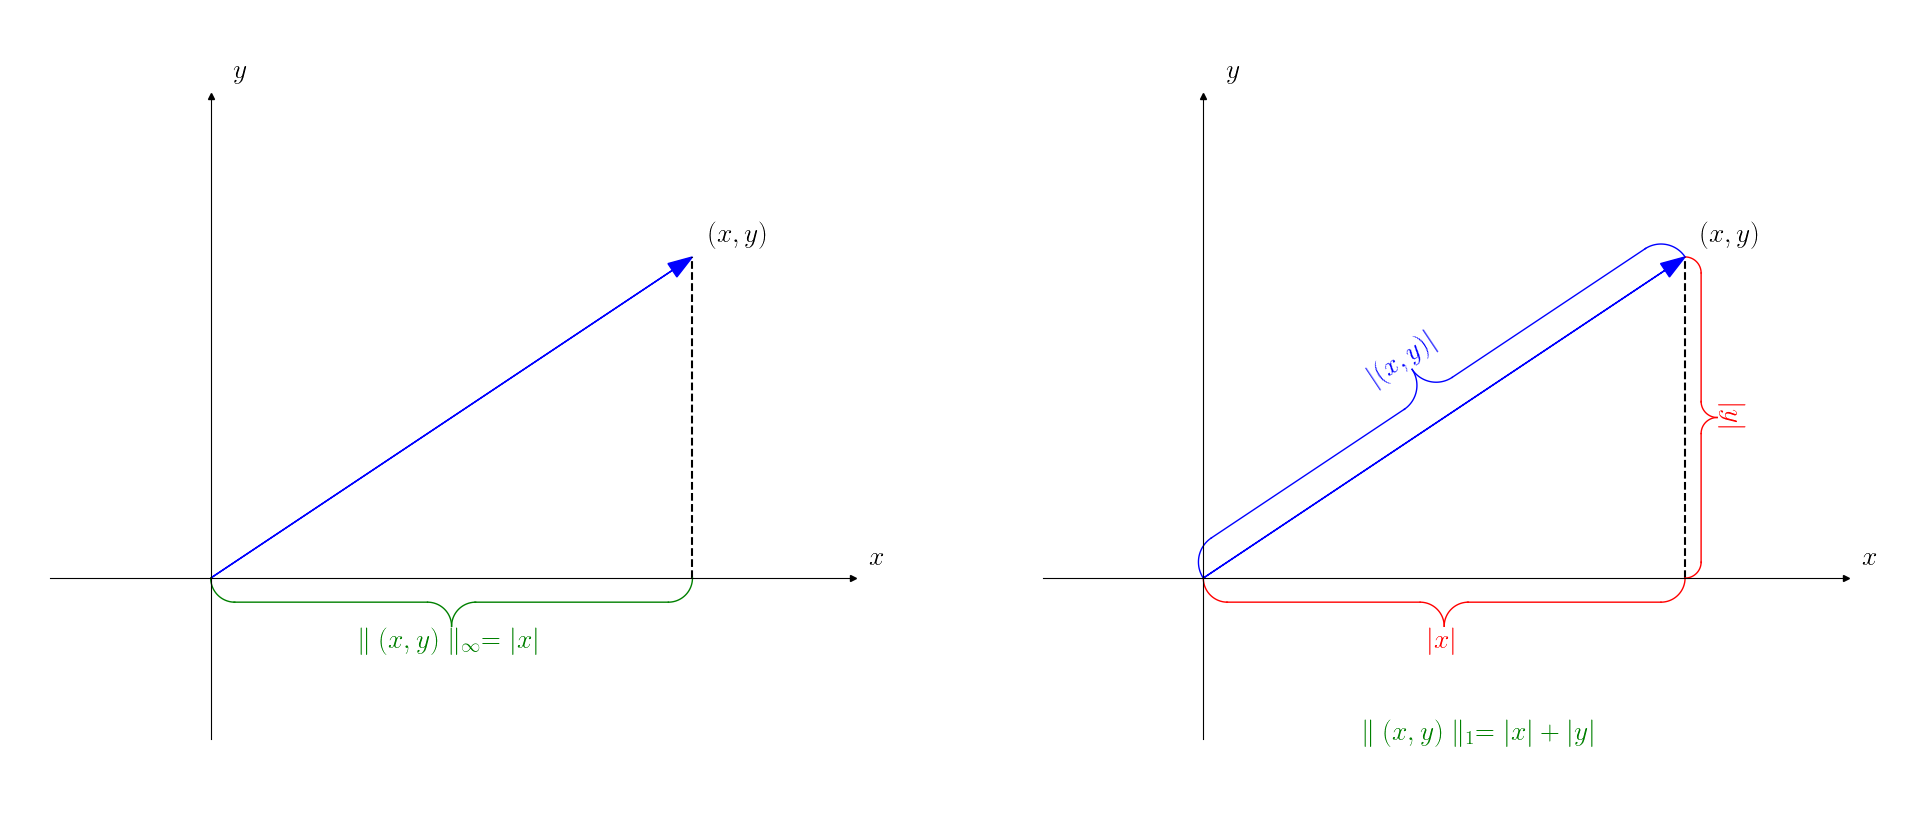
\includegraphics[width=\linewidth]{spazi_metrici_e_normati/pag126}
		\label{fig:pag126}
	\end{center}
	\begin{gather*}
		\parallel \overline{x} \parallel_p = \left( \sum_{i=1}^{n} |x_i|^p \right)^{\frac{1}{p}} \quad p \geq 1
		\\
		\parallel \overline{x} \parallel_\infty = \lim_{p \rightarrow +\infty} \parallel \overline{x} \parallel_p
	\end{gather*}
	$(\mathbb{R}^n, \parallel \cdot \parallel_p)$ è spazio normato

	\item $C^0 \left( [0,1] \right)$
	\begin{align*}
		&\parallel f \parallel_\infty = \sup_{x \in [0,1]} |f(x)| (=\max_{x \in [0,1]} |f(x)|)
		\\
		&\parallel f \parallel_1 = \int_{0}^{1} |f(x)| \ \mathrm{d}x
		\\
		&\parallel f \parallel_p = \left( \int_{0}^{1} |f(x)|^p \ \mathrm{d}x \right)^{\frac{1}{p}} \qquad p \geq 1
	\end{align*}

sono tute norme su $C^0 ([0,1])$
\end{itemize}
\end{exbar}


\begin{exbar}
\begin{example}
	Facciamo vedere che $\parallel \cdot \parallel_\infty$ su $C^0 ([0,1])$ è una norma
	\begin{enumerate}
		\item $\parallel f \parallel_\infty \geq 0 \qquad$ (banale)
		
		$\parallel f \parallel_\infty =  0 \iff f(x) = 0 \qquad \forall \ x \in [0, 1]$
		
		$\parallel f \parallel_\infty =  0 \iff \sup_{x \in [0,1]} |f(x)| = 0$
		
		$\iff 0 \leq |f(x)| \leq 0 \quad \forall \ x \in [0,1] \iff f(x) = 0 \qquad \forall \ x \in [0,1]$
		
		\item $\parallel \lambda f \parallel_\infty = |\lambda| \parallel f \parallel_\infty \qquad \forall \lambda \in \mathbb{R}$ e $\forall f \in C^0 ([0,1])$
		
		$\parallel \lambda f \parallel_\infty = \sup_{x \in[0,1]} |\lambda f(x)| = \sup_{x\in[0,1]} |\lambda| \ |f(x)| = |\lambda| \sup_{x\in[0,1]} |f(x)| = |\lambda| \parallel f \parallel_\infty$
		
		\item $\parallel f+g \parallel_\infty \leq \parallel f \parallel_\infty + \parallel g \parallel_\infty \qquad \forall f,g \in C^0 ([0,1])$
		
		$\parallel f+g \parallel_\infty = \sup_{x\in[0,1]} |f(x) + g(x)|$
		
		$|f(x) + g(x)| \distr |f(x)| + |g(x)| \leq \sup_{y\in[0,1]} |f(y)| + \sup_{y\in[0,1]} |g(y)| =  \parallel f \parallel_\infty + \parallel g \parallel_\infty \ \forall \ x \in [0,1]$
		
		$\parallel f+g \parallel_\infty = \sup_{x\in[0,1]} |f(x) + g(x)| \leq \parallel f \parallel_\infty + \parallel g \parallel_\infty$
	\end{enumerate}
\end{example}
\end{exbar}
	

\begin{exbar}
\begin{example}
		Facciamo vedere che $\parallel f\parallel_1 = \int_{0}^{1} |f(x)| \ \mathrm{d}x$
		
		è una norma
	\begin{enumerate}
		\item $\parallel f \parallel_1 \geq 0 \qquad \forall f \in C^0 ([0,1]) \text{ banale}$
		
		Dimostriamo che $\parallel f \parallel_1 = 0 \iff f(x) = 0 \qquad \forall \ x \in [0,1]$
		
		$\Leftarrow) f(x) = 0 \qquad \forall \ x \in[0,1]$
		
		$\parallel f \parallel_1 = \int_{0}^{1} 0 \ \mathrm{d}x = 0$
		
		$\Rightarrow)$ Sia $\parallel f \parallel_1 = 0$ e dimostriamo che $f(x) = 0 \qquad \forall \ x \in [0,1]$
		
		$\int_{0}^{1} |f(x)| \ \mathrm{d}x = 0$
		
		Se $\exists \ x_0 \in [0,1]$ tale che $|f(x_0)| \neq 0$ allora $\exists$ un intorno $U$ di $x_0 $ tale che $|f(x)| \geq \frac{|f(x_0)|}{2}$ $\qquad \forall x \in U \cap [0,1]$ 
		
		\begin{itemize}
			\item $U = \ ]x_0 - \delta, x_0 + \delta[ \ \subseteq [0,1]$
	
			\item $x_0=0$
			
			$U= \ ]0 - \delta, 0 + \delta[$
			
			$U \cap [0,1] = [0, \delta[$
			
			\item $x_1 = 1$
			 $U= \ ]1 - \delta, 1 + \delta[$
			 
			$U \cap [0, 1] = \ ]1 - \delta, 1]$
		\end{itemize}
		
		cioè in ogni caso $U \cap [0,1]$ è un intervallo di ampiezza almeno $\frac{\delta}{2}>0$
		
		\begin{equation*}
			\parallel f\parallel_1 = \int_{0}^{1} |f(x)| \ \mathrm{d}x \geq \int_{U \cap [0,1]} |f(x)| \ \mathrm{d}x \geq \int_{U \cap [0,1]} \frac{|f(x_0)|}{2} \ \mathrm{d}x \geq \frac{\delta}{4} |f(x_0)| > 0
		\end{equation*}
		
		il che è assurdo, perché $\parallel f\parallel_1 = 0$
		
		\item $\parallel \lambda f \parallel_1 = \int_{0}^{1} |\lambda f(x)| \ \mathrm{d}x = |\lambda| \int_{0}^{1} |f(x)| \ \mathrm{d}x = |\lambda| \parallel f \parallel_1 \qquad \lambda \in \mathbb{R}$
		
		\item $f,g \in C^0 ([0,1])$
		
		$\parallel f+g \parallel_1 = \int_{0}^{1} |f(x) + g(x)| \ \mathrm{d}x \leq \int_{0}^{1} (|f(x)| + |g(x)|) \ \mathrm{d}x = \parallel f \parallel_1 + \parallel g \parallel_1$
		
		$\Rightarrow$ vale la disuguaglianza triangolare
	\end{enumerate}
\end{example}
\end{exbar}


\begin{attbar}
	Dato uno spazio normato $(X, \parallel \cdot \parallel)$ posso definire la distanza tra due vettori $x,y \in X$ come $d(x,y)= \parallel x-y \parallel$, lunghezza del vettore $x-y$
	\begin{center}
		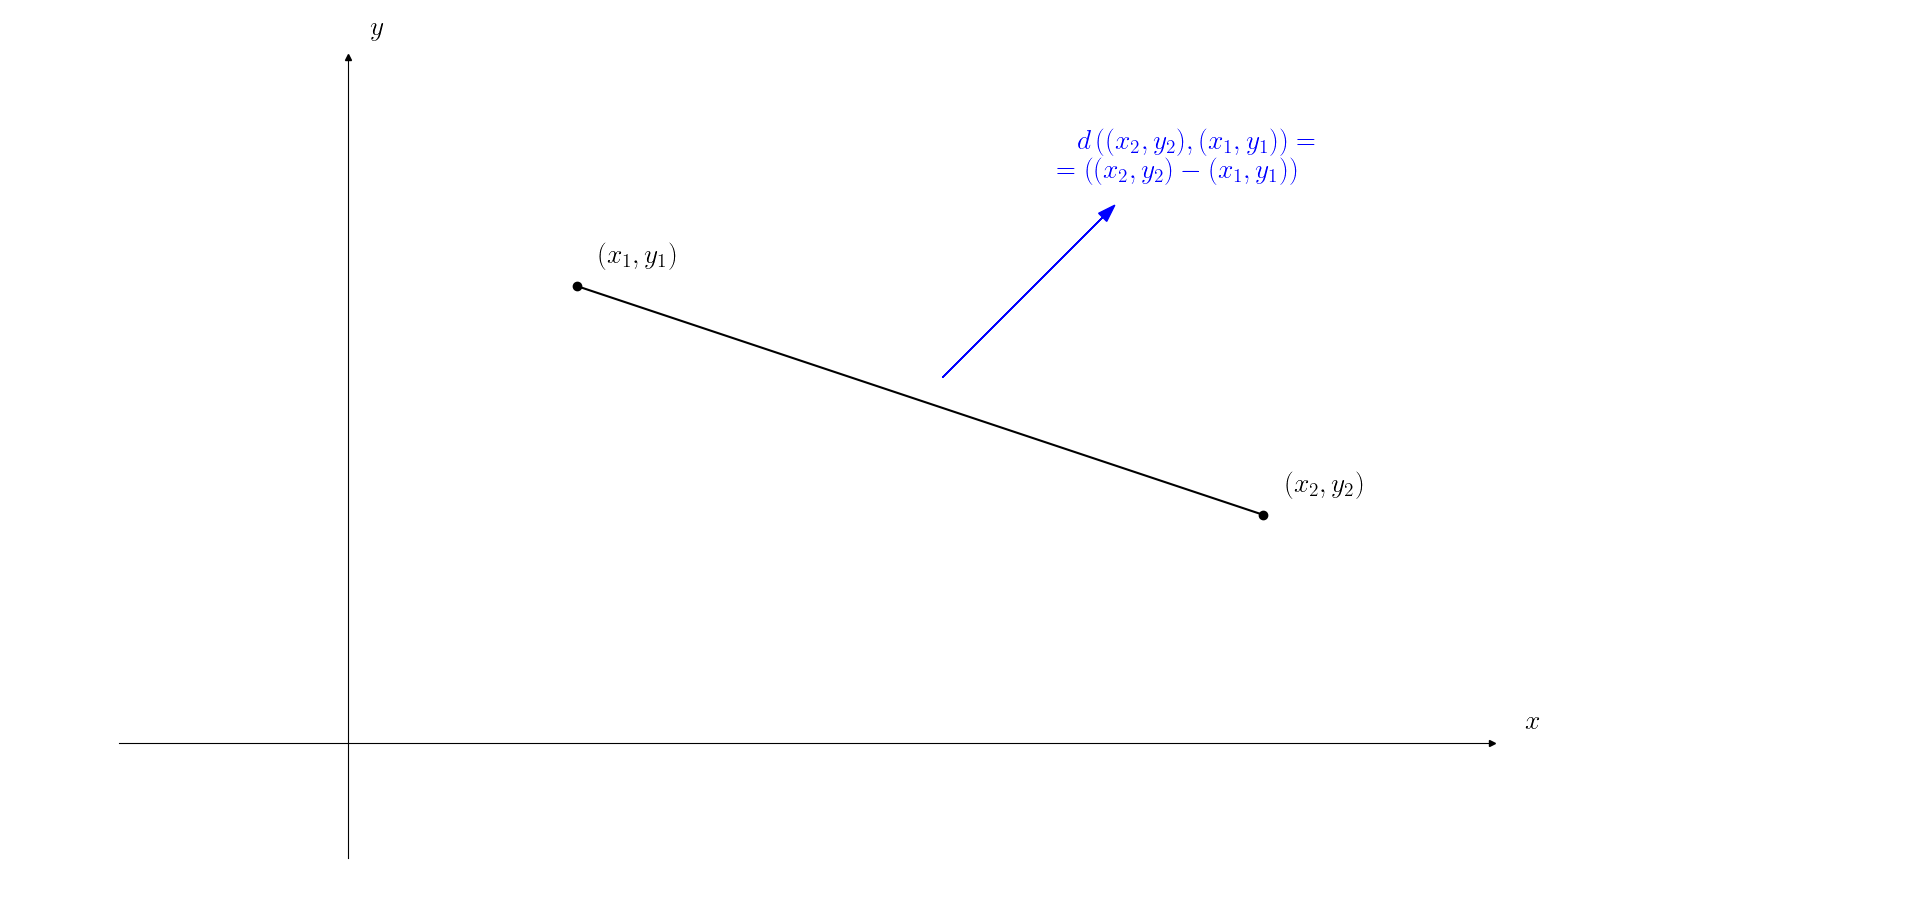
\includegraphics[width=0.75\linewidth]{spazi_metrici_e_normati/pag131}
		\label{fig:pag131}
	\end{center}
\end{attbar}


\begin{definition}
	$X$ insieme non vuoto. Una distanza o metrica su $X$ è una funzione \\ %riq malf
	$d:X \times X \rightarrow \mathbb{R}$ tale che
	\begin{enumerate}
		\item $d(x,y) \geq 0 \qquad \forall \ x,y \in X $ e $d(x,y) = 0 \iff x = y$
		\item $d(x,y) = d(y,x)$ (proprietà simmetrica)
		\item Disuguaglianza triangolare $d(x,y) \leq d(x,z) + d(z,y) \qquad \forall \ x,y,z \in X$
	\end{enumerate}
	
	La coppia $(X,d)$ si dice \textbf{spazio metrico}.
\end{definition}



$(X, \parallel \cdot \parallel)$ normato

$d(x,y)=\parallel x-y \parallel$ è metrica, allora
\begin{enumerate}
	\item $d(x,y)\geq 0$ banalmente 
	$d(x,y) = \parallel x-y \parallel = 0 \iff x-y = 0 \iff x = y$
	\item $d(x,y) = \parallel x-y \parallel = \parallel y-x \parallel = d(y,x)$
	\item $d(x,y) = \parallel x-y \parallel = \parallel (x-z) + (z-y) \parallel \leq \parallel x-z \parallel + \parallel z-y \parallel = d(x,z) + d(y,z)$
\end{enumerate}

Dato uno spazio vettoriale $X$ e $d$ metrica su $X$, esiste una norma $\parallel \cdot \parallel$ su $X$ tale che $d(x,y) = \parallel x-y \parallel$?

No, esistono metriche dentro lo spazio vettoriale che non derivano da una norma.


\begin{exbar}
\begin{example}
	$\mathbb{R}, \quad 0 < p < 1 , \quad d(x,y) = |x-y|^p$. 
	
	Allora $d$ è una metrica, che non deriva da una norma.
	
	Se esistesse una norma $\parallel \cdot \parallel$ su $\mathbb{R}$ tale che $d(x,y) = \parallel x-y \parallel$, allora, fissato $\lambda \in \mathbb{R}$,
	\begin{gather*}
		d(\lambda x, \lambda y) = \parallel \underbrace{\lambda x - \lambda y}_{\lambda (x - y)} \parallel \uppercomment{=} {\text{seconda}} {\text{proprietà di }\parallel \cdot \parallel} |\lambda| \parallel x-y \parallel = |\lambda | \ d(x,y)
		\\
		d(\lambda x, \lambda y) = |\lambda x - \lambda y|^p = |\lambda|^p |x-y|^p = |\lambda|^p d(x,y) \neq |\lambda| \ d(x,y) \text{ se } |\lambda \neq 1,0|
	\end{gather*}
	
	Facciamo vedere che $d(x,y) = |x-y|^p$ è una distanza, $0 < p < 1$
	\begin{enumerate}
		\item $d(x,y) \geq 0$ banale
		
		$d(x,y) = 0 \iff |x-y|^p = 0 \iff |x-y| = 0 \iff x = y$
		
		\item $d(x,y) = d(y,x)$ banale
		
		\item Disuguaglianza triangolare
		
		Dobbiamo dimostrare che $\forall \ x,y,z \in \mathbb{R}$ vale
		\begin{gather*}
			d(x,y) \leq d(x,z) + d(z,y)
			\\
			|x-y|^p \leq |x-z|^p + |z-y|^p
			\\
			|x-y|^p \distr (|x-z| + |y-z|)^p
		\end{gather*} 
	
		Se dimostro che $( \underbrace{|x-z|}_{= a} + \underbrace{|y-z|}_{=b})^p \leq |x-z|^p + |z-y|^p$, sono a posto $\forall \ x,y,z \in \mathbb{R}$ con $0<p<1$.
		
		Devo dunque dimostrare che $(a+b)^p \leq a^p + b^p \qquad \forall \ a,b \in \mathbb{R}^{\geq 0}$.
		
		Se $a=0$ o $b=0$, banale
		
		Siano $a,b \neq 0$
		\begin{gather*}
		(a + b)^p \leq a^p + b^p \qquad /.\frac{1}{b^p}
		\\
		\iff \frac{(a+b)^p}{b^p} \leq \frac{a^p}{b^p} + 1 \iff \left( \frac{a+b}{b} \right)^p \leq \left( \frac{a}{b} \right)^p + 1 \iff
		\\
		\iff \left( \frac{a}{b} + 1 \right)^p \leq \left( \frac{a}{b} \right)^p + 1 \qquad \forall \ a,b > 0
		\end{gather*}
		
		Posto $\lambda = \frac{a}{b}>0$
		\begin{gather*}
		\left( \frac{a}{b} + 1 \right)^p \leq \left( \frac{a}{b} \right)^p + 1 \qquad \forall \ a,b>0 \iff (\lambda + 1)^p \leq \lambda^p + 1 \qquad \forall \ \lambda > 0
		\\
		(\lambda + 1)^p - \lambda^p \leq 1
		\\
		f(\lambda) = (\lambda + 1)^p -\lambda^p \qquad f:\mathbb{R}^{\geq 0} \rightarrow \mathbb{R}
		\\
		f(\lambda) \leq 1 = f(0)
		\\
		f'(\lambda) 
		\lowercomment{=} {\myarrow[270]} {\lambda \neq 0} p \ (\lambda + 1)^{p - 1} - p \ \lambda^{p - 1} 
		= p \ [(\lambda + 1)^{p - 1} - \lambda^{p - 1}] 
		= p \ \lambda^{p - 1} \left[ \left( \frac{\lambda + 1}{\lambda} \right)^{p-1} - 1 \right] 
		\\
		=  p \ \lambda^{p - 1} \left[ \underbrace{ \left(  1 + \frac{1}{\lambda} \right) ^{\overbrace{p - 1}^{<0}} }_{<1} - 1 \right] < 0 \qquad \forall \ \lambda > 0
 		\end{gather*}
		
		$f$ è decrescente e quindi $\forall \ \lambda > 0 \Rightarrow f(\lambda) \leq f(0)$, come si voleva.
	\end{enumerate}
\end{example}
\end{exbar}


\subsection{Topologia}

$(X,d)$ spazio metrico.

\begin{definition}
	
\end{definition}
	Sia $x \in X, r >0$, allora $B_r(x) = \{ y \in X | d(x,y) < r \}$ si dice \textbf{palla (aperta)} di centro $x$ e raggio $r$.

	
\begin{exbar}
	\begin{gather*}
		(\mathbb{R}^2, | \cdot |), \qquad \mathbb{R}^2 \text{ con norma euclidea}
		\\
		B_r (0,0), \qquad r > 0
		\\
		B_r (0,0) 
		= \{ (x,y) \in \mathbb{R}^2 \big| d((x,y), (0,0)) < r \} 
		= \{ (x,y) \in \mathbb{R}^2 \big| |(x,y)-(0,0)| < r \} =
		\\ 
		= \{ (x,y) \in \mathbb{R}^2 \big| \sqrt{x^2+y^2} < r\}
	\end{gather*}
	\begin{center}
		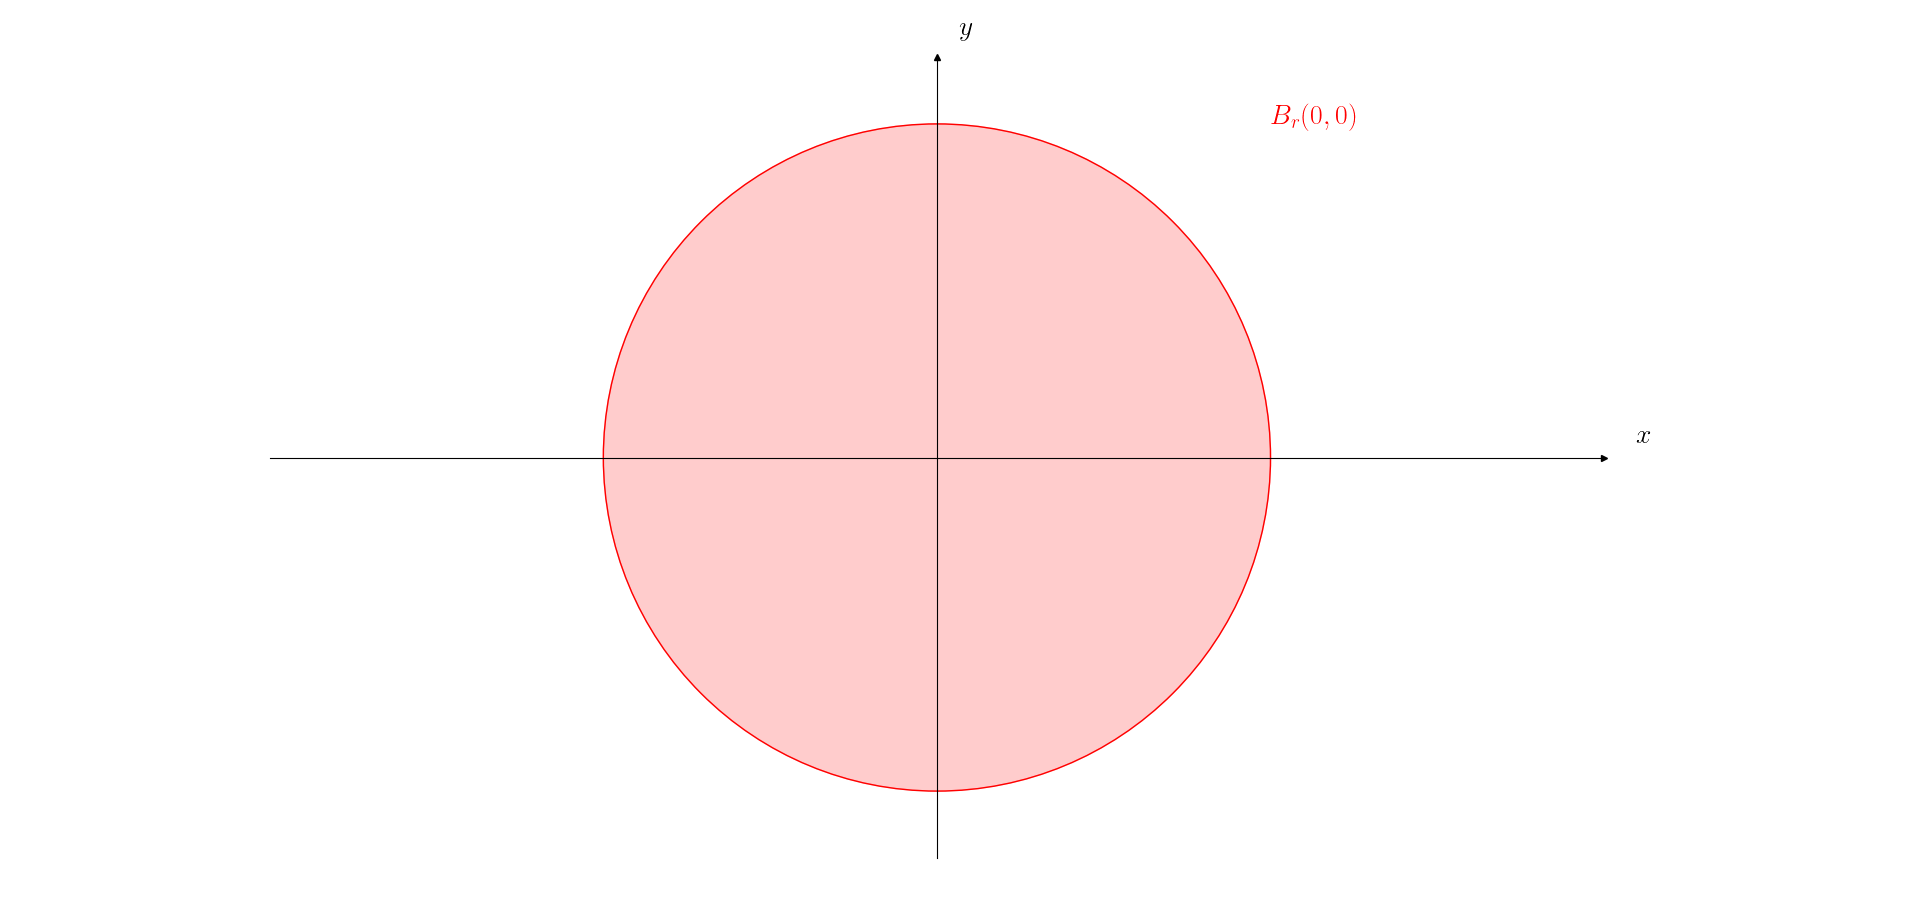
\includegraphics[width=0.75\linewidth]{spazi_metrici_e_normati/pag137circle}
		\label{fig:pag137circle}
	\end{center}
	
	\begin{gather*}
	 	(\mathbb{R}^2, \parallel \cdot \parallel_\infty)
	 	\\
		\parallel (x,y) \parallel_\infty = \max \{|x|,|y|\} 
		\\
		B_r^\infty (0,0) 
		= \{ (x,y) \in \mathbb{R}^2 \big| \parallel(x,y) - (0,0) \parallel_\infty < r \} 
		= \{ (x,y) \in \mathbb{R}^2 \big| \max \{|x|,|y| \} < r \} =
		\\
		= \{ (x,y) \in \mathbb{R}^2 \big| |x|,|y| < r\}
	\end{gather*}
	\begin{center}
		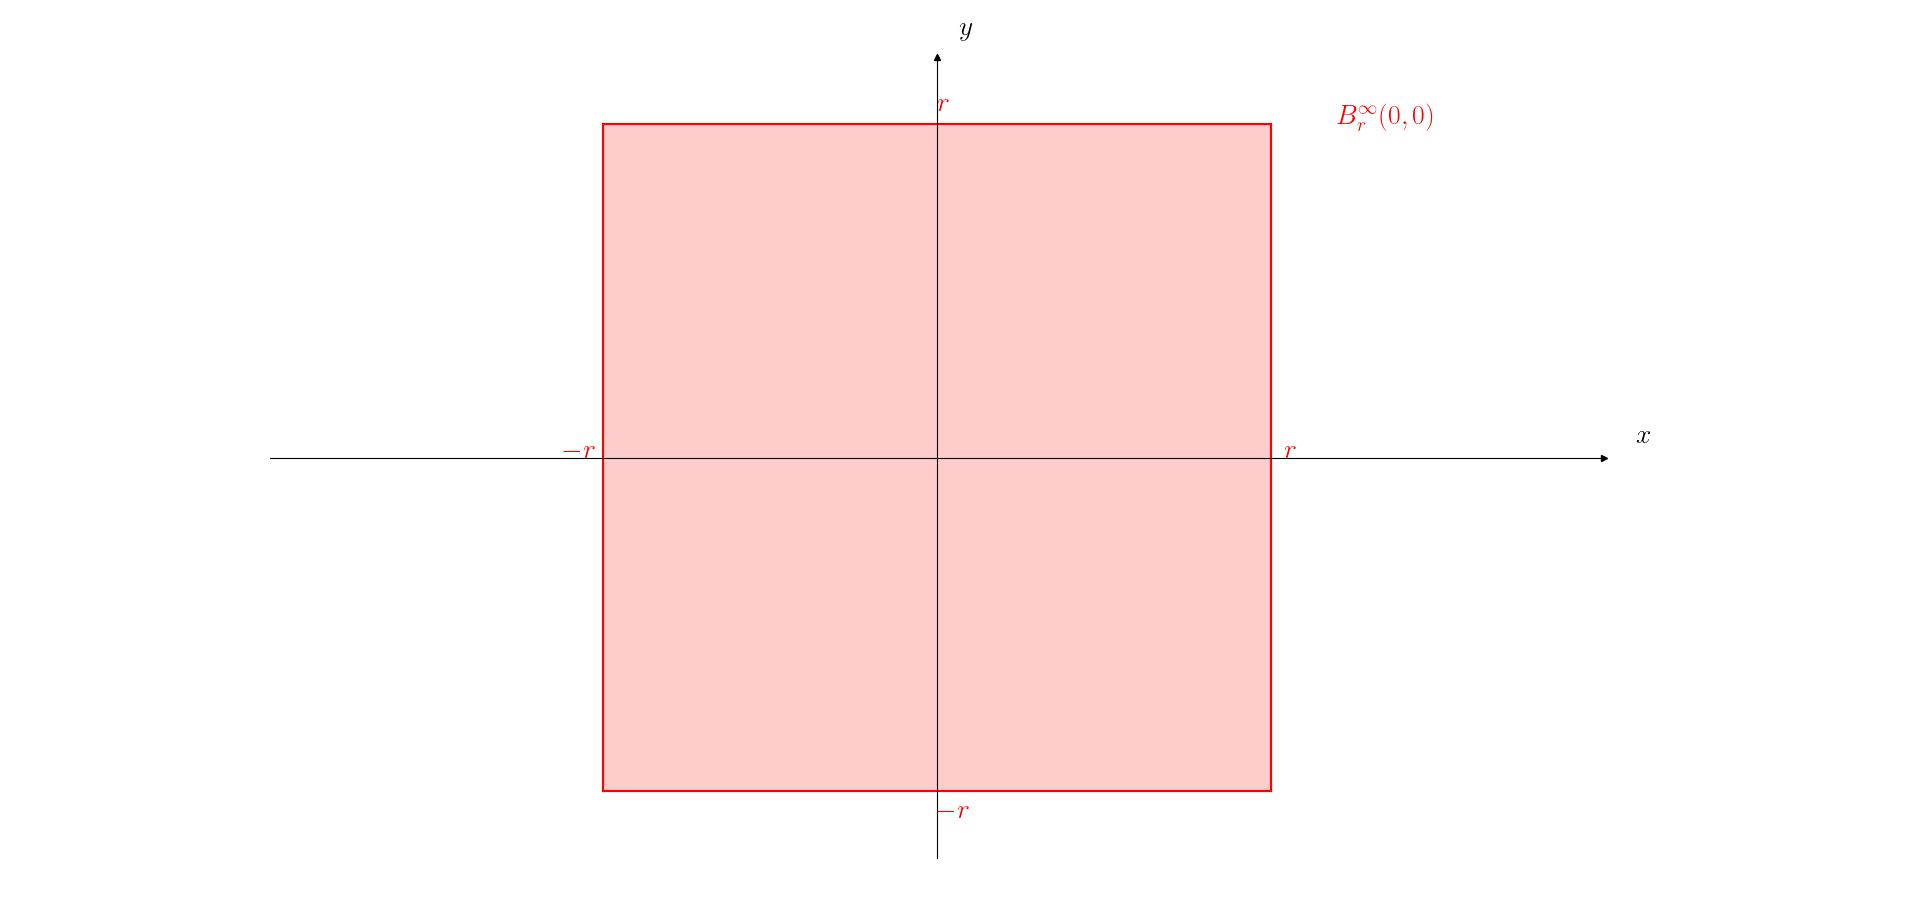
\includegraphics[width=0.75\linewidth]{spazi_metrici_e_normati/pag137square}
		\label{fig:pag137square}
	\end{center}
	
	\begin{gather*}
		(\mathbb{R}^2, \parallel \cdot \parallel_1)
		\qquad
		\parallel (x,y) \parallel_1 = |x| + |y| 
		\\
		B_r^1 (0,0) = \{(x,y) \in \mathbb{R}^2 \big| \parallel (x,y) - (0,0) \parallel_1 < r \} 
		= \{(x,y) \in \mathbb{R}^2 \big| |x| + |y| < r \}
	\end{gather*}
	\begin{center}
		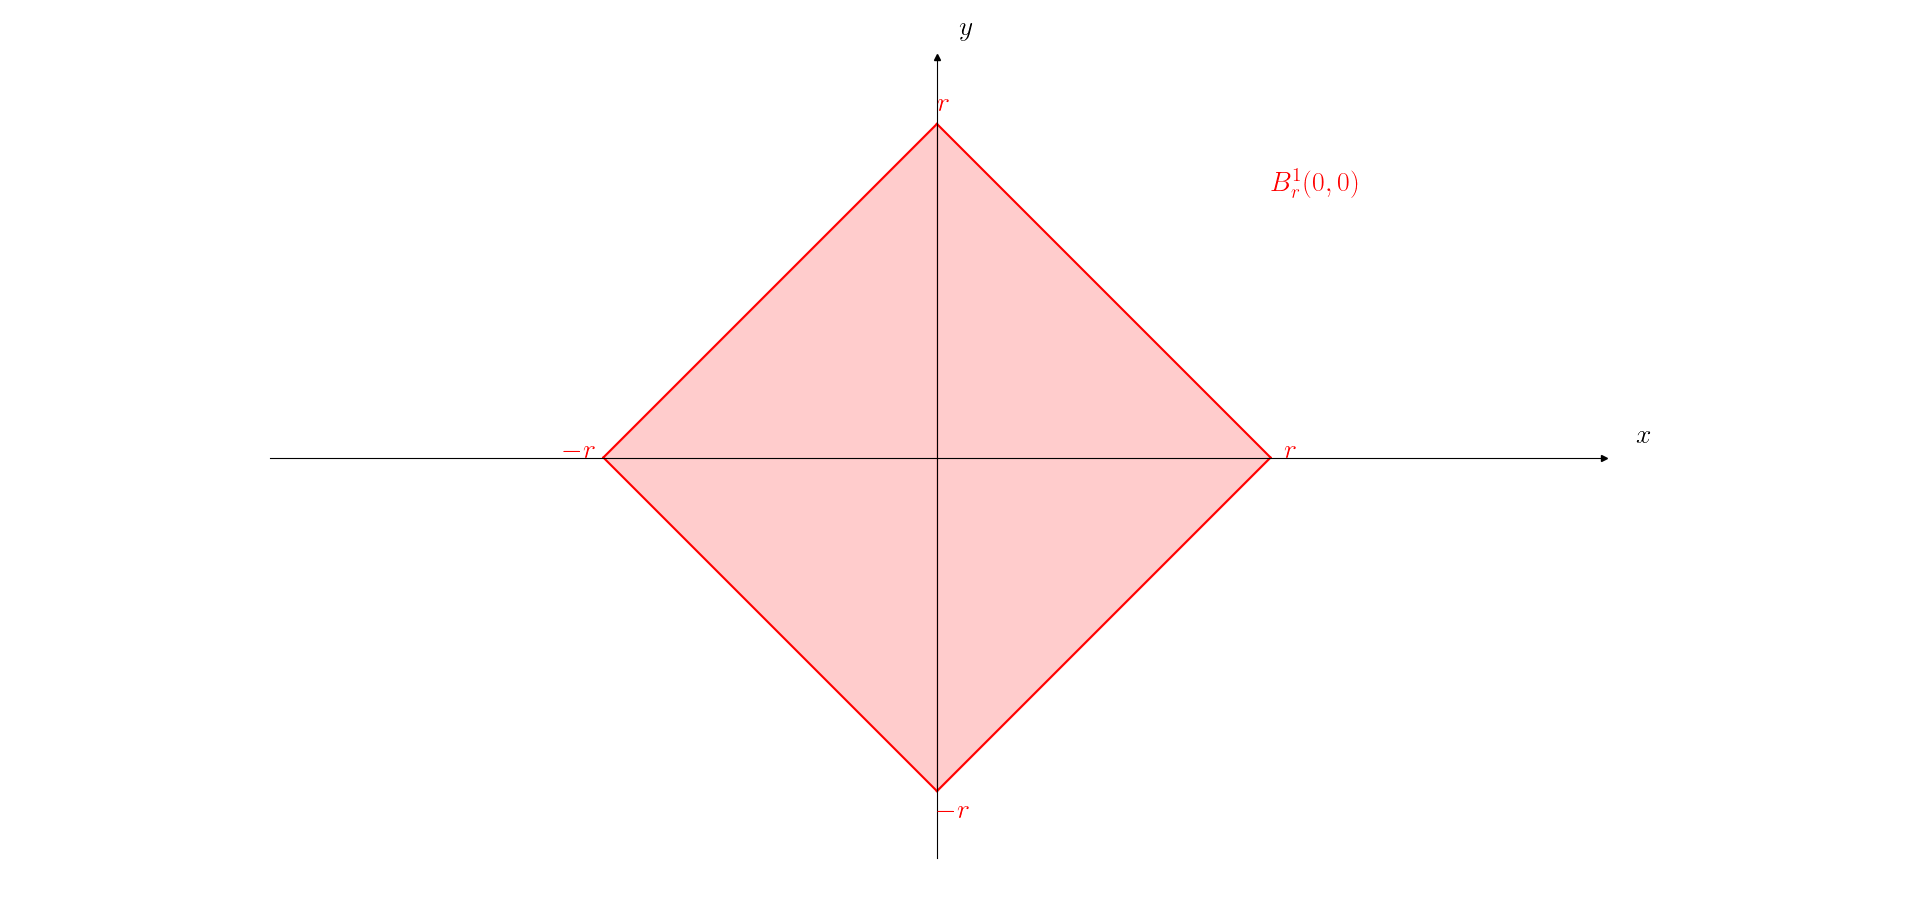
\includegraphics[width=0.75\linewidth]{spazi_metrici_e_normati/pag138rhombus}
		\label{fig:pag138rhombus}
	\end{center}

	\begin{gather*}
		(C^\circ([0,1]), \parallel \cdot \parallel_\infty) \qquad
		d(f,g) = \parallel f-g \parallel_\infty
		\\
		f \in C^0 (), \qquad r>0
		\\
		B_r^\infty(f) = \{ g \in C^0 ([0,1]) \big| \parallel f-g \parallel_\infty < r \} = \{ g \in C^0 ([0,1]) \big| \undercomment{\sup_{x \in [0,1]} |f(x) - g(x)|} {f(x) - r < g(x) < f(x) + r} {} < r \} 
	\end{gather*}		
	\begin{center}
		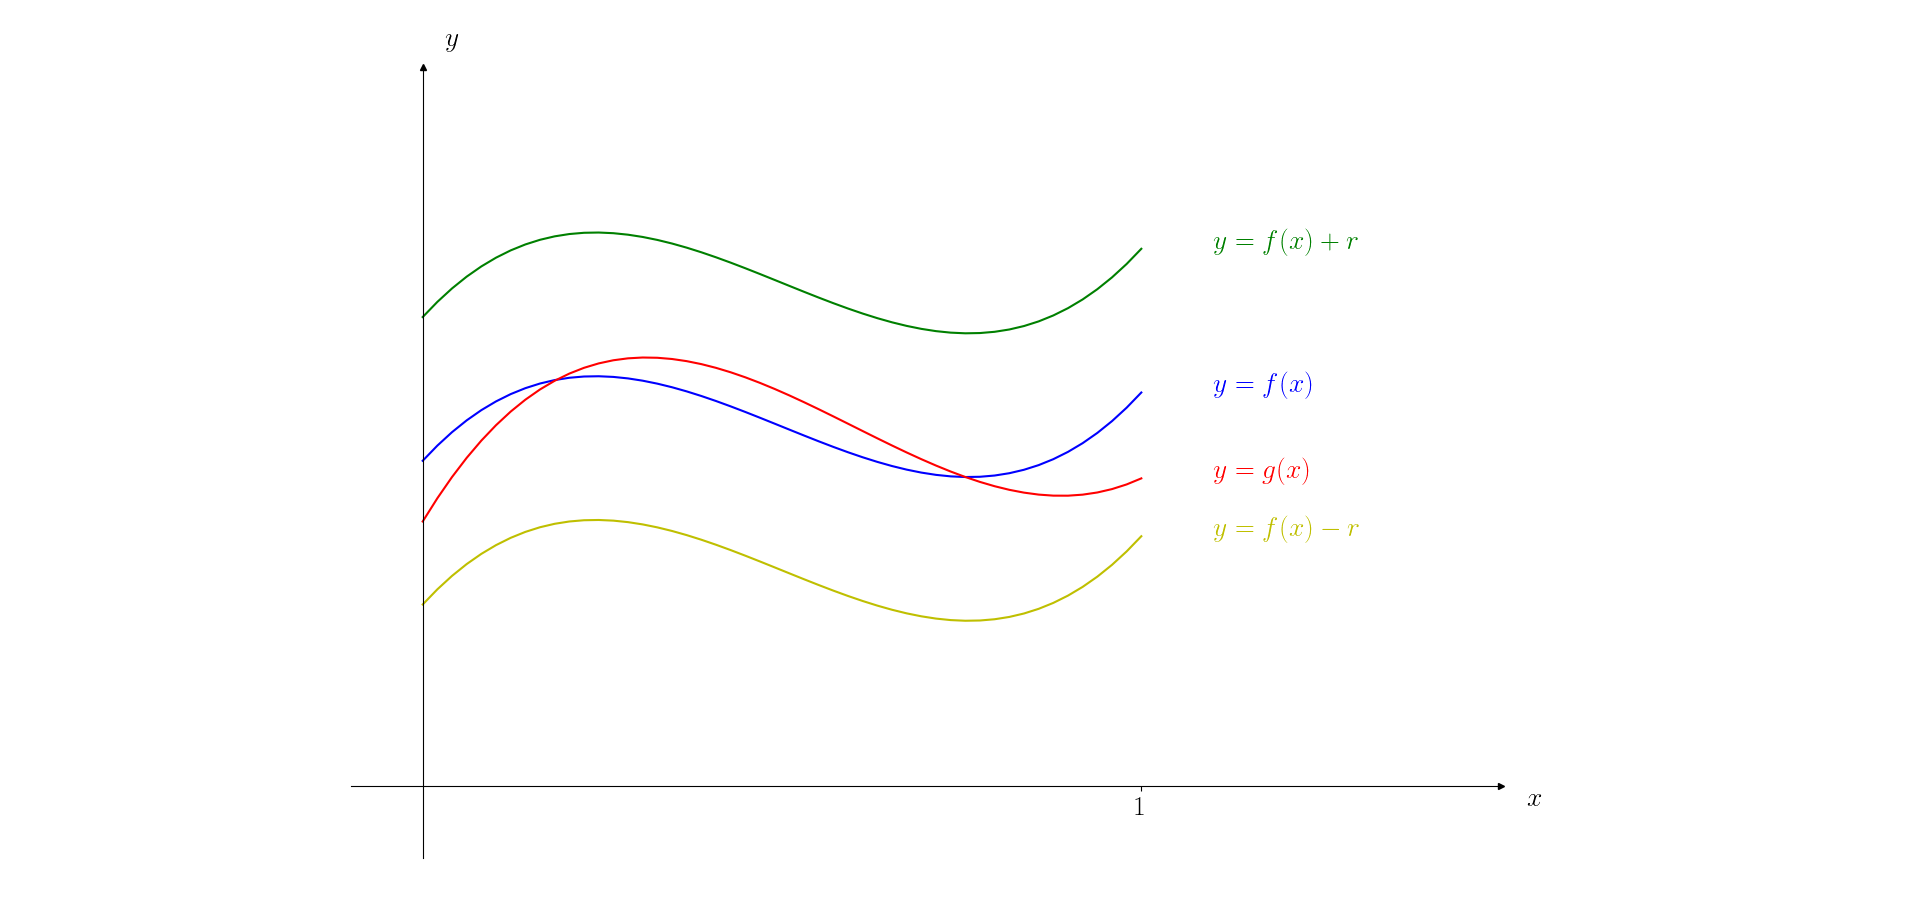
\includegraphics[width=0.75\linewidth]{spazi_metrici_e_normati/pag138curve}
		\label{fig:pag138curve}
	\end{center}
	
	$$f(x)=0 \qquad \forall \ x \in [0,1]$$
	\begin{center}
		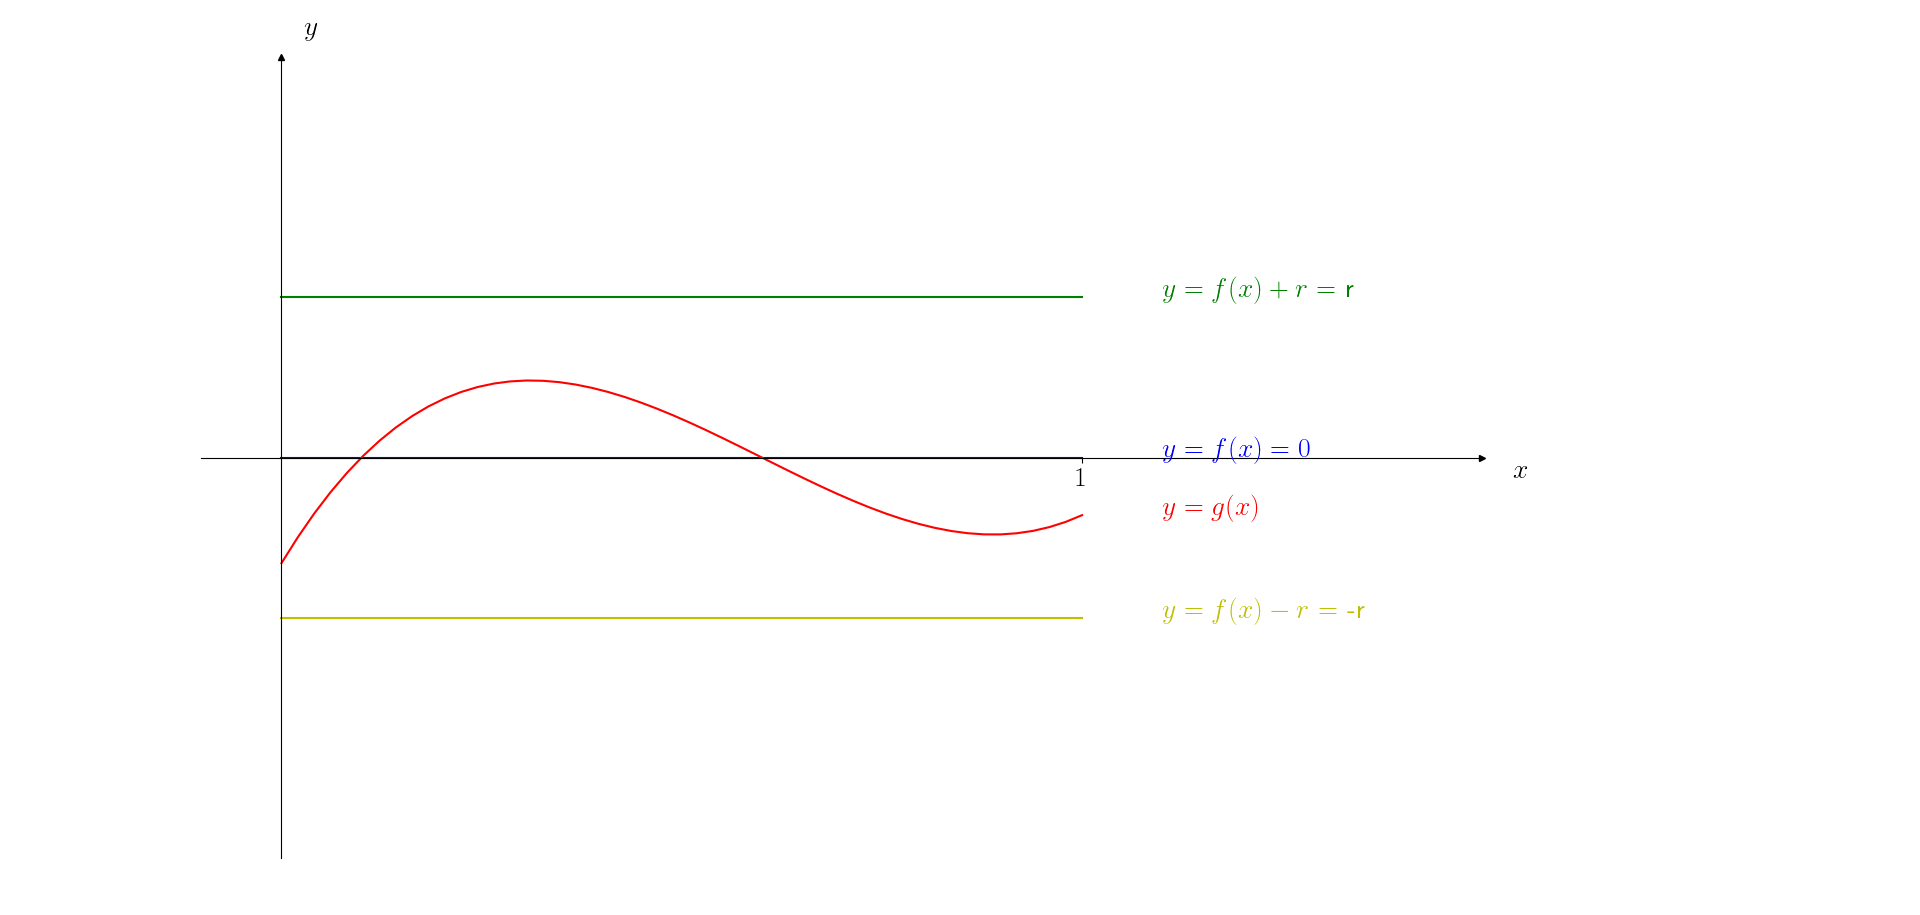
\includegraphics[width=0.65\linewidth]{spazi_metrici_e_normati/pag139curve}
		\label{fig:pag139curve}
	\end{center}
	
	\begin{gather*}
		C^0 ([0,1]), \parallel \cdot \parallel_1
		\\
		\parallel f \parallel_1 = \int_{0}^{1} |f(x)| \ \mathrm{d}x 
		\\
		B_r^1 = \{ g \in C^0 ([0,1]) \big| \parallel f-g \parallel_1 < r \} = \{g \in C^0 ([0,1]) \bigg| \int_{0}^{1} |f(x) - g(x)| \ \mathrm{d}x < r \}
		\\
		f(x) = 0 \qquad \forall \ x \in [0,1]
		\\
		B_r^1(0) = \{ g \in C^0 ([0,1]) \bigg| \int_{0}^{1} |g(x)| \ \mathrm{d}x < r \}
	\end{gather*}
	\begin{center}
		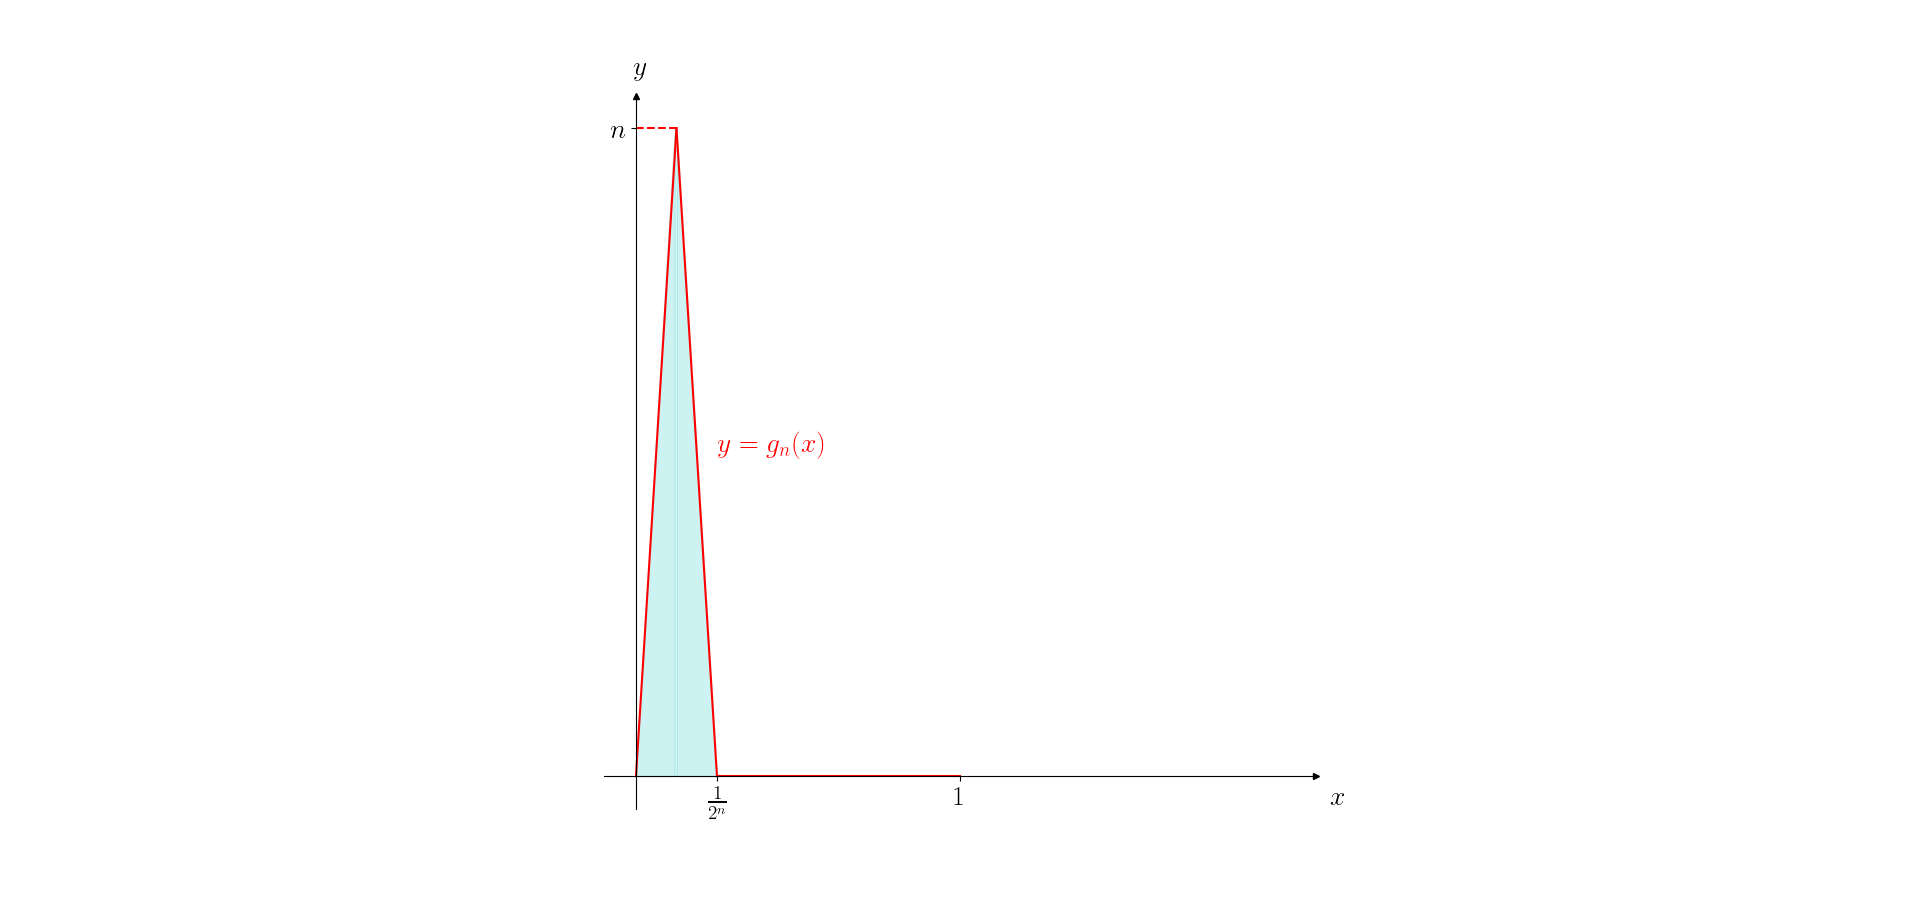
\includegraphics[width=0.85\linewidth]{spazi_metrici_e_normati/pag139triangolo}
	\end{center}

	$\int_{0}^{1} |g_n(x)| \ \mathrm{d}x =$ area del triangolo $ = \frac{1}{2} \frac{1}{2^n} n = \lowercomment{\frac{n}{2^{n+1}}} {\myarrow[270]} {0 \text{ per } n \rightarrow + \infty}$

	Fissato $r > 0$, trovo $n$ tale che $\int_{0}^{1} |g_n(x)| \ \mathrm{d}x < r$	
\end{exbar}


\begin{definition}
	$x \in X$. Un \textbf{intorno di $x$} è un qualsiasi sottoinsieme $A \subseteq X$ che contiene una palla aperta centrata in $x$, cioè per cui $\exists \ r > 0 \big| B_r(x) \subseteq A$
\end{definition}


\begin{definition}
	$A \subseteq X$ si dice \textbf{aperto} se è intorno di ogni suo punto, cioè se $\forall \ x \in A \quad \exists r > 0 \ \big|$ $B_r(x) \subseteq A$.
	
	$A$ si dice \textbf{chiuso} se $A^c = X \backslash A$ è aperto.
\end{definition}


\begin{exbar}
\begin{example}
	$(x,d)$ spazio metrico, $x \in X, r>0$, $B_r(x)$ è un aperto.
	
	Devo far vedere che $\forall \ y \in B_r(x) \ \exists \ \overline{r} > 0 \ \big| \; B_{\overline{r}}(y) \subseteq B_r(x)$
	
	$\overline{r} = r - d(x,y) > 0$ perché $d(x,y) < r$ e dimostriamo che, se $z \in B_{\overline{r}} (y)$, allora $z\in B_r(x)$, cioè, se $d(y,z)< \overline{r}$, allora $d(x,z)<r$
	
	$d(x,z) \distr  d(x,y) + d(y,z) < d(x,y) + \overline{r} = d(x,y) + (r-d(x,y)) = r$	
	\begin{center}
		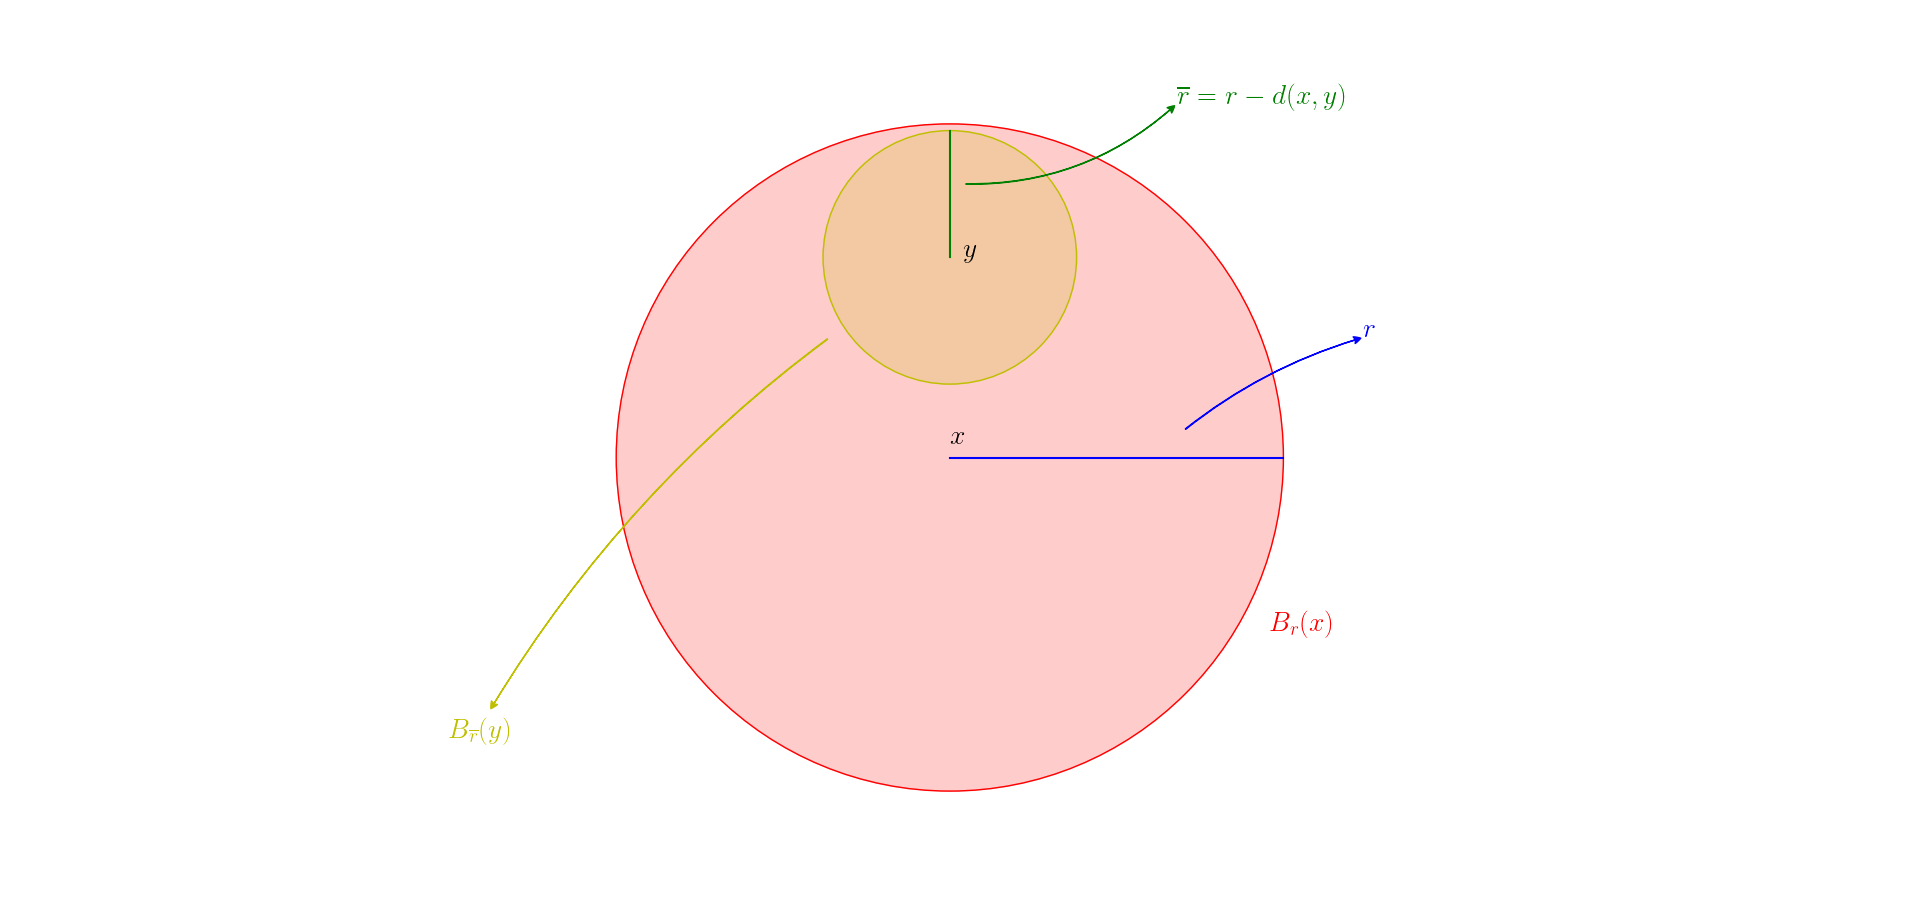
\includegraphics[width=0.75\linewidth]{spazi_metrici_e_normati/pag141}
		\label{fig:pag141}
	\end{center}
\end{example}
\end{exbar}


\begin{exbar}
	$(\mathbb{R}^2, \parallel \cdot \parallel_\infty)$
	\begin{center}
		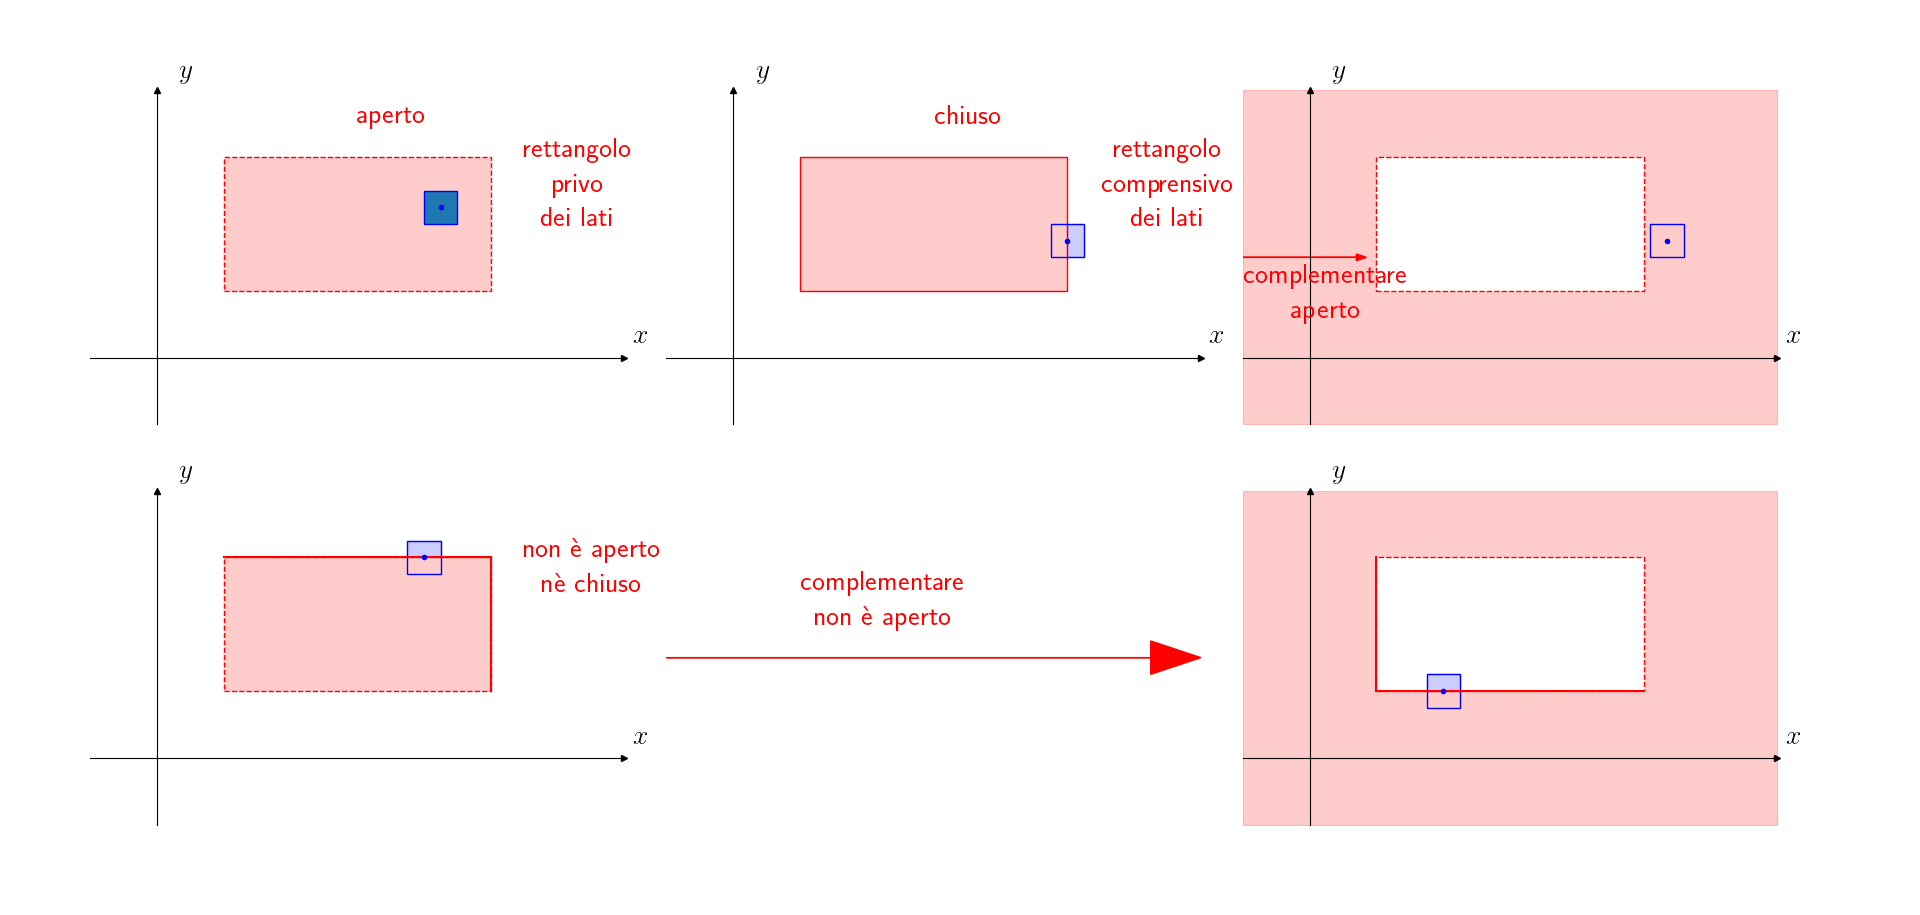
\includegraphics[width=\linewidth]{spazi_metrici_e_normati/pag141-142}
		\label{fig:pag141-142}
	\end{center}
\end{exbar}


\textbf{Osservazione:} 
	$(X,d)$ spazio metrico, $X$ è aperto banalmente (se $x \in X, B_r(x) \subseteq X \ \forall \ r > 0$) e quindi $\emptyset = X^c = X \backslash X$ è chiuso. 
	
	D'altra parte $\emptyset $ è aperto perché l'implicazione $x \in \emptyset \Rightarrow  \ \exists \ r > 0 \ \big| \ B_r(x) \subseteq \emptyset$ è vera perché $x \in \emptyset$  è falsa $\Rightarrow \emptyset^c = X \backslash \emptyset = X$ è chiuso. 
	
	\begin{attbar}
		$\emptyset, X$ sono sia aperti che chiusi.
	\end{attbar}


\begin{theorem}
	
	$(X,d)$ spazio metrico
	\begin{enumerate}
		\item $A_1, A_2 \subseteq X$ aperti $\Rightarrow A_1 \cap A_2$ è un aperto.
		 
		\item $\{A_i\}_{i \in I}$ è una famiglia di aperti, allora $\bigcup_{i \in I} A_i$ è un aperto.
		
		\item Se $C_1, C_2 \subseteq X$ sono chiusi, allora $C_1 \cup C_2$ è chiuso.
		
		\item $\{C_i\}_{i\in I}$ è famiglia di chiusi, allora $\bigcap_{i \in I} C_i$ è un chiuso.
	\end{enumerate}
\end{theorem}


\textbf{Osservazione:} 
In generale se $\{ A_i \}_{i \in I}$ è una famiglia infinita di aperti, allora $\bigcap_{i \in I} A_i$ non è un aperto e, se $\{ C_i \}_{i \in I}$ è una famiglia infinita di chiusi, allora $\bigcup_{i \in I} C_i$ non è chiuso. Facciamo un esempio.

$A_k= \ \bigg]-\frac{1}{k}, \frac{1}{k} \bigg[ \qquad k \geq 1, k \in \mathbb{N}$ sono tutti aperti di $\mathbb{R}$, allora $\bigcap_{k=1}^\infty A_k = \bigcap_{k=1}^\infty \ \bigg] -\frac{1}{k}, \frac{1}{k} \bigg[ \ = \{ 0 \}$, che è un chiuso.

$C_k = \left[ \frac{1}{k}, 1-\frac{1}{k} \right], \qquad k \geq 2, k \in \mathbb{N}$ sono tutti chiusi 

\bigg( $C_k^c = \ \bigg] -\infty, \frac{1}{k} \bigg[ \ \cup \ \bigg] 1-\frac{1}{k}, +\infty \bigg[$, unione di due intervalli aperti \bigg)

$\bigcup_{k=2}^\infty C_k = \bigcup_{k=2}^\infty \left[ \frac{1}{k}, 1-\frac{1}{k} \right] = \ ]0,1[$

Infatti, se $x \in \bigcup_{k=1}^\infty \left[ \frac{1}{k}, 1-\frac{1}{k} \right]$, allora $\exists \ \overline{k} \geq 2 \ \big| \ \left[\frac{1}{k}, 1-\frac{1}{k}\right]$, cioè $0 < \frac{1}{k} \leq x \leq 1- \frac{1}{k} < 1$

$\Rightarrow 0 < x < 1 \Rightarrow x \in \ ]0,1[.$

D'altra parte, se $x \in \ ]0,1[$, esistono $k_1$ e $k_2 \ \big| \ \frac{1}{k_1} < x<1 - \frac{1}{k_2}$

$k=\max\{k_1, k_2\}$ 

\begin{gather*}
	\frac{1}{k} \leq \frac{1}{k_1} < x < 1 - \frac{1}{k_2} \leq 1 - \frac{1}{k}
	\\
	\Rightarrow x \in C_k = \left[ \frac{1}{k}, 1 - \frac{1}{k} \right]
	\\
	\Rightarrow x \in \bigcup_{k=2}^{\infty} C_k
\end{gather*}


\begin{definition}
	
	$(X,d)$ spazio metrico, $A \subseteq X, \ x \in A$. $x$ si dice \textbf{punto interno di A} se $\exists \ r > 0 \ \big| \ B_r(x) \subseteq A$. L'interno di $A$ è l'insieme dei punti interni di $A$ ed è indicato con \AA
\end{definition}


\begin{proposition}
	\label{pr: grande aperto}
	\AA \ è un insieme aperto ed è il più grande aperto, nel senso dell'inclusione, contenuto in $A$, cioè se $B \subseteq A$ è aperto, allora $B \subseteq$ \AA
\end{proposition}

\begin{dembar}
	\textbf{Dimostrazione} della \textbf{Proposizione \ref{pr: grande aperto}} (Esercizio per casa)
\end{dembar}


\begin{exbar}
	\begin{gather*}
		A = \ ]0,1], \qquad \text{\AA} = \ ]0,1[
		\\
		A = \ ]0,1] \cup \{ 2 \}, \qquad \text{\AA} = \ ]0,1[
		\\
		A = \ ]0,1] \cup \left\{2 + \frac{1}{n} \ \bigg| \ n \geq 1, n \in \mathbb{N} \right\}, \qquad \text{\AA} = \ ]0,1[
	\end{gather*}
\end{exbar}


\begin{definition}
	$A \subseteq X, x \in X$ si dice \textbf{punto di chiusura} per $A$ se $B_r(x) \cap A \neq \emptyset \ \forall \ r > 0$, cioè ogni palla di centro $x$ interseca $A$. 
	
	La chiusura di $A$ è l'insieme di tutti i punti di chiusura di $A$ ed è denotata con $\overline{A}$.
\end{definition}


\begin{proposition}
	\label{pr: grande chiuso}
	$\overline{A} $ è un insieme chiuso ed è il più piccolo chiuso, nel senso dell'inclusione, contenente $A$, cioè, se $C \geq A$ è chiuso, allora $\overline{A} \subseteq C$
\end{proposition}


\begin{dembar}
	\textbf{Dimostrazione} della \textbf{Proposizione \ref{pr: grande chiuso}} (Esercizio per casa)
\end{dembar}


\begin{exbar}
	\begin{gather*}
		A = \ ]0,1], \qquad \lowercomment{\overline{A} = [0,1]} {0 \notin A, \text{ mentre se } x \in \text{\AA} \Rightarrow x \in A} {x \in A \Rightarrow x \in \overline{A} \text{ perché } x \in B_r(x) \cap A \ \forall r > 0}
		\\
		A = \ ]0,1] \cup \{ 2 \}, \qquad \overline{A} = [0,1] \cup \{ 2 \}
		\\
		A = \ ]0,1] \cup \left\{ 2 + \frac{1}{n} \ \bigg| \ n \geq 1, n \in \mathbb{N} \right\}, \qquad \overline{A} = [0,1] \cup \left\{2 + \frac{1}{n} \ \bigg| \ n \geq 1, n \in \mathbb{N} \right\} \cup \{ 2 \}	
	\end{gather*}
\end{exbar}


\textbf{Osservazione:}
\begin{gather*}
	\text{\AA} \subseteq A \subseteq \overline{A}
	\\	
	A \text{ è aperto } \iff A = \text{\AA}
	\\
	A \text{ è chiuso } \iff A = \overline{A}
\end{gather*}

$(\Leftarrow) A=\overline{A}$, $\overline{A}$ è un chiuso $\Rightarrow A$ è chiuso

$(\Rightarrow)$ Sia $A$ chiuso e dimostriamo che $A = \overline{A}$. Noi sappiamo che $A \subseteq \overline{A}$.

Se per assurdo $A \nsubseteq \overline{A}, \; \exists \ x \in \overline{A} \ \big| \ x \notin A$, cioè $x \in \overline{A}$ e $x \in A^c$. Ma $ A^c $ è aperto, perché $ A $ è chiuso, e quindi $ \exists r > 0 \ \big| \ B_r (x) \subseteq A^c$

$\Rightarrow B_r (x) \cap A = \emptyset$, assurdo perché $x \in \overline{A}$.


\begin{definition}
	$A \subseteq X, x \in X$ si dice \textbf{punto di frontiera} per $A$ se $\forall \ r > 0 \quad B_r(x) \cap A \neq \emptyset$ e $B_r(x) \cap A^c \neq \emptyset$, cioè se ogni palla di centro $x$ interseca sia $A$ che il suo complementare.
	
	L'insieme dei punti di frontiera di $A$ si dice frontiera di $A$ e si indica con $\partial A$. 
\end{definition}


\begin{exbar}
	\begin{gather*}
		A = ]0,1], \qquad \partial A = \{0,1\} 
		\\
		A = \ ]0,1] \cup \{ 2 \}, \qquad \partial A = \{ 0, 1, 2 \}
		\\
		A = \ ]0,1] \cup \left\{ 2 + \frac{1}{n} \ \bigg| \ n \geq 1, n \in \mathbb{N} \right\}, \qquad \partial A = \{0,1\} \cup \left\{2 + \frac{1}{n} \ \bigg| \ n \geq 1, n \in \mathbb{N} \right\} \cup \{ 2 \}
	\end{gather*}
$(\mathbb{R}^2, \parallel \cdot \parallel_\infty)$
g
\begin{center}
	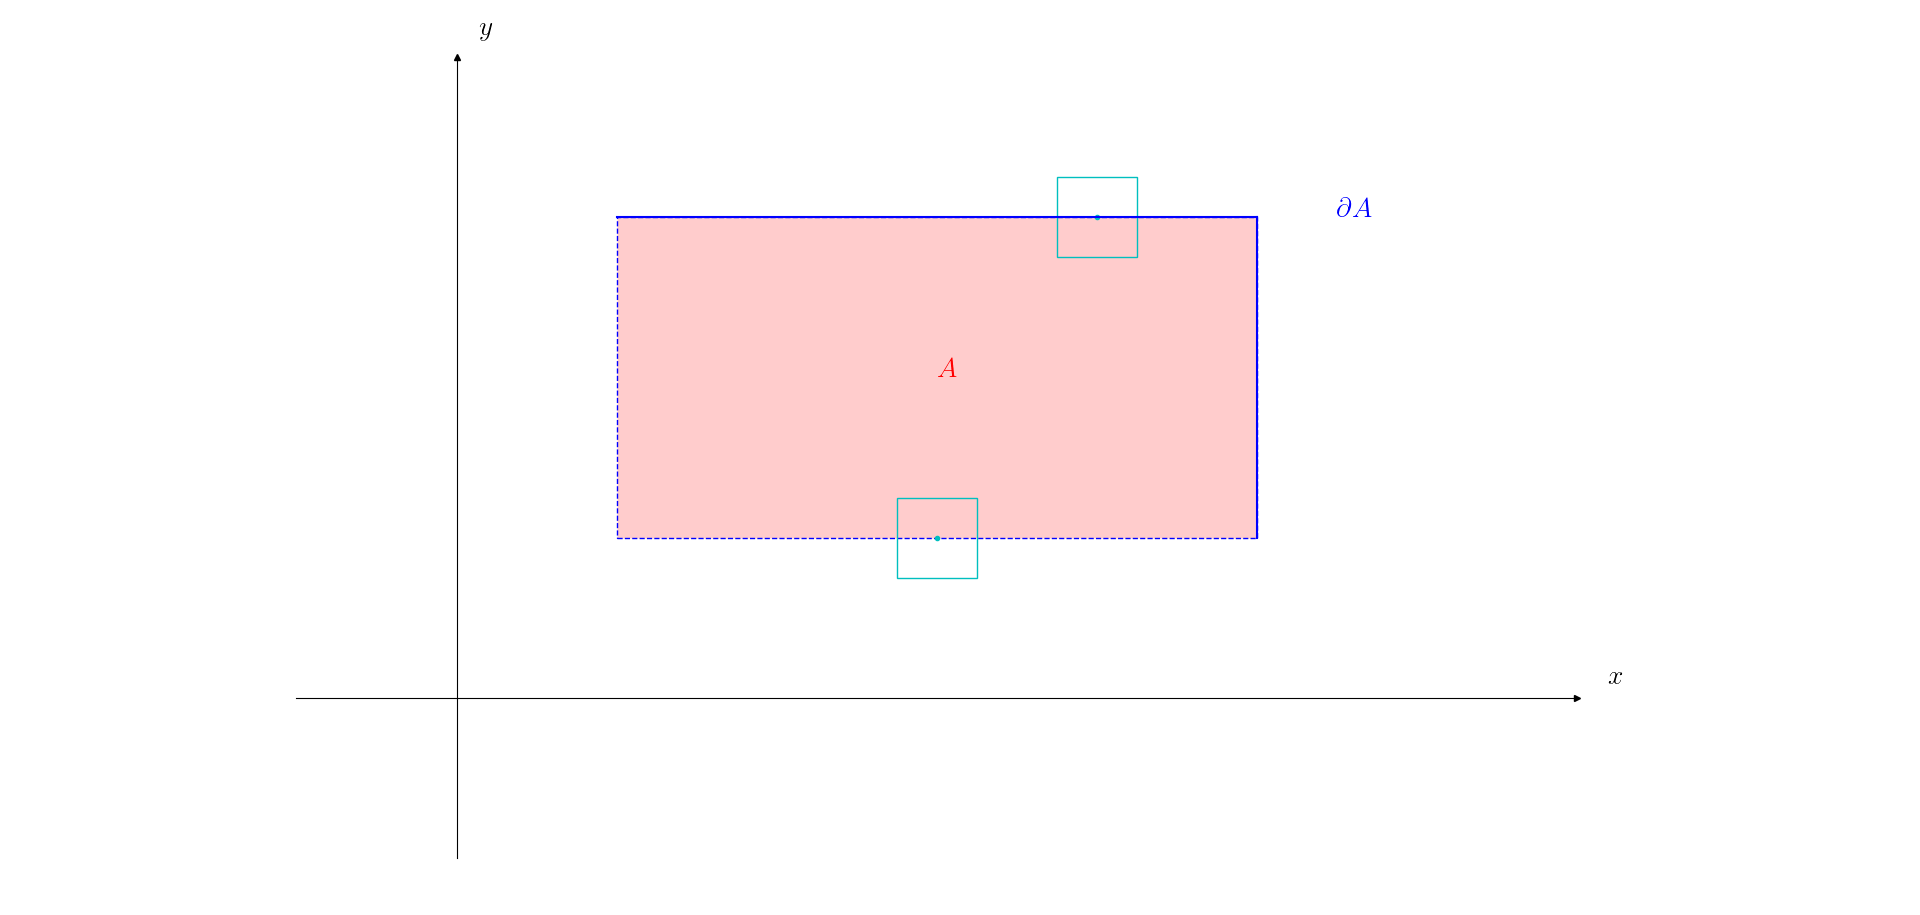
\includegraphics[width=0.65\linewidth]{spazi_metrici_e_normati/pag148}
	\label{fig:pag148}
\end{center}
\end{exbar}


\textbf{Osservazione:}

\begin{itemize}
\item $\partial A = \overline{A} \cap \overline{A^c}$
\begin{gather*}
	x \in \partial A \Rightarrow B_r (x) \cap A \neq \emptyset \qquad \forall \ r > 0, \; x \in \overline{A}
	\\
	\Rightarrow B_r(x) \cap A^c \neq \emptyset \qquad \forall r > 0, \; x \in \overline{A^c}
	\\
	\Rightarrow x \in \overline{A} \cap \overline{A^c} \Rightarrow \partial A \subseteq \overline{A} \cap \overline{A^c}
	\\
	x \in \overline{A} \cap \overline{A^c} \Rightarrow x \in \overline{A} \text{ e } x \in \overline{A^c}
	\\
	\begin{array}{c c}
		x \in \overline{A} \Rightarrow B_r(x) \cap A \neq \emptyset \quad \forall \ r > 0
		\\
		x \in \overline{A^c} \Rightarrow B_r(x)\cap A^c \neq \emptyset \quad \forall \ r > 0
	\end{array}
	\Rightarrow x \in \partial A
	\\
	\Rightarrow \overline{A} \cap \overline{A^c} \subseteq \partial A
\end{gather*}

\item $\overline{A}=A \cup \partial A$

\begin{equation*}
	A \subseteq \overline{A}, \; \partial A \subseteq \overline{A} \Rightarrow A \cup \partial A \subseteq \overline{A}
\end{equation*}
Facciamo vedere che $\overline{A} \subseteq A \cup \partial A$.
	
$x \in \overline{A}$, supponiamo che $x \notin A$ e dimostriamo che $x \in \partial A$
	
\begin{gather*}
	x \in \overline{A}  \Rightarrow \lowercomment{B_r(x) \cap A \neq \emptyset} {(x \notin A \Rightarrow x \in A^c)} {} \qquad \forall \ r > 0
	\\
	x \in B_r (x) \cap A^c \qquad \forall \ r > 0
	\\
	\mathcircled{B_r(x) \cap A^c \neq \emptyset \qquad \forall \ r > 0}
	\\
	\Rightarrow x \in \partial A, \text{ come si voleva}
\end{gather*}
\end{itemize}


\begin{attbar}
	$A$ è chiuso $\iff \partial A \subseteq A$, cioè se e solo se $A$ contiene la sua frontiera.
\end{attbar}


\begin{exbar}
\begin{example}
	$(\mathbb{R}, |\cdot|), \qquad \mathbb{Q} \subseteq \mathbb{R}$
	
	\begin{gather*}
		\overline{\mathbb{Q}} = \mathbb{R}
		\\
		\text{Fissati } x\in \mathbb{R} \text{ e }  r > 0 \quad \exists \ q \in \mathrm{Q} \text{ tale che }  q \in \ ]x-r, x+r[ \ = B_r(x)
		\\
		\partial \mathbb{Q} = \mathbb{R}
		\\
		x \in \mathbb{R}, \ B_r(x) \cap \mathbb{Q} \neq \emptyset \qquad \forall \ r > 0, B_r(x) \cap \ \mathbb{Q}^c \neq \emptyset \qquad \forall \ r > 0
		\\
		]x-r,x+r[ \ \cap \mathbb{Q}^c \neq \emptyset \qquad \forall \ r > 0
	\end{gather*}
	
	Se non fosse vero, $\exists \ x \in \mathbb{R}$ e $r > 0$ tale che $]x-r, x+r[$ è fatto tutto di numeri razionali.
	
	I razionali sono numerabili, cioè $\exists f: \mathbb{N} \rightarrow \mathbb{Q} $ iniettiva e suriettiva. I reali hanno la potenza del continuo, cioè ogni funzione $\phi: \mathbb{N} \rightarrow \mathbb{R}$ può essere al più iniettiva, ma non suriettiva. Questo è vero anche per ogni intervallo del tipo $]x-r, x+r[, r > 0$. Quindi, se $]x-r, x+r[$ fosse fatto di soli numeri razionali, sarebbe numerabile, assurdo.
\end{example}
\end{exbar}


\subsection{Successioni in spazi metrici}
\begin{exbar}
\begin{itemize}
	\item $\mathbb{R}^2 \qquad \{(e^{-n}, \frac{\sin n}{n}) \}_{n\geq 1}$ è una successione di elementi di $\mathbb{R}^2$
	\item $\mathbb{R}^3 \qquad \{ (1+\frac{1}{n}, \frac{\sinh n}{e^n},2^{-n}) \}$ è una successione di elementi di $\mathbb{R}^3$
\end{itemize}
\end{exbar}


\begin{definition}
	$\{x_k\}_{k\in \mathbb{N}} \subseteq X$ successione, con $(X,d)$ spazio metrico. 
	
	Si dice che $\{ x_k\}_{k \in \mathbb{N}}$ converge ad $x \in X$ e si scrive
	\begin{equation*}
		x_k \rightarrow x \qquad \text{o} \qquad \lim_{k\rightarrow +\infty} x_k = x \iff \lim_{k \rightarrow +\infty} d(x_k, x) = 0
	\end{equation*}
	
	(in ambito reale $\lim_{k \rightarrow +\infty} |x_k - x |=0$)
	
	cioè $\iff \forall \ \epsilon > 0 \ \exists \ N > 0 \ \big| \ k > N$
	
	$\Rightarrow d(x_k,x) < \epsilon$
	
	$x$ viene detto \textbf{limite della successione}.
	
\end{definition}


\begin{theorem}
	Sia $\{ x_k \}_{k \in \mathbb{N}} \subseteq X, (X,d)$ spazio metrico, tale che 
	\begin{equation*}
		x_k \rightarrow l_1 \in X \text{ e } x_k \rightarrow l_2 \in X
	\end{equation*}
	
	Allora $l_1=l_2$.
\end{theorem}


\begin{proposition}
	\label{pr:pag152}
	$\{\overline{x_k}\}_{k \in \mathbb{N}} \subseteq R^n$ tale che $\overline{x_k } = (x_{k_1}, x_{k_2}, \ldots, x_{k_n})$. Allora
	\begin{equation*}
		\overline{x_k} \rightarrow \overline{x} = (x_1, \ldots, x_n) \iff x_{k_{j}} \rightarrow x_{j} \qquad \forall \ j = 1, \ldots, n
	\end{equation*}
	
	cioè $\iff \forall \ j = 1, \ldots, n$ la successione di numeri reali $\{ x_{kj} \}_{k \in \mathbb{N}}$ converge a $x_{j}$.
\end{proposition}


\begin{exbar}

\begin{itemize}
	\item $\mathbb{R}^2, \left\{ \underbrace{ \left(e^{-k}, \frac{\sin k}{k} \right)} _ {\overline{x_k}} \right\}_{k \geq 1}$
	\begin{gather*}
		\overline{x_k} = (x_{k_1}, x_{k_2})
		\\
		\begin{array}{c c}
			x_{k_1} = e^{-k}, &
			x_{k_2} = \frac{\sin k}{k}
			\\
			\lim_{k \rightarrow +\infty} x_{k_1}=0, & \lim_{k \rightarrow +\infty} x_{k_2} = 0
		\end{array}
		\\
		\Rightarrow \lim_{k \rightarrow + \infty} \overline{x_k} = (0,0)
	\end{gather*}
	
	\item $\mathbb{R}^3, \left\{ \underbrace{ \left(1 + \frac{1}{k}, \frac{\sinh k}{e^k}, 2^{-k} \right)} _ {\overline{x_k}} \right\}_{k \geq 1}$
	\begin{gather*}
		\begin{array}{c c c}
		x_{k_1} = 1 + \frac{1}{k}, 
		& x_{k_2} = \frac{\sinh k}{e^k}, 
		& x_{k_3} = 2^{-k}
		\\
		\lim_{k \rightarrow +\infty} x_{k_1} = 1, \quad
		& \lim_{k \rightarrow +\infty} x_{k_2} = 1, \quad 
		& \lim_{k \rightarrow +\infty} x_{k_3} = 0 
	\end{array}
		\\
		\lim_{k \rightarrow +\infty} \overline{x_k} = (1, 1, 0)
	\end{gather*}

	\item $\mathbb{R}^2, \left\{ \underbrace{(2+e^{-k}, \sin k)} _ {\overline{x_k}} \right\} $
	\begin{gather*}
	\begin{array}{c c}
		x_{k1} = 2+e^{-k}, \quad 
		& x_{k2} = \sin k
		\\
		\lim_{k \rightarrow +\infty} x_{k_1} = 2, \quad 
		& \lim_{k \rightarrow +\infty} \nexists
	\end{array}
		\\
		\Rightarrow \lim_{k \rightarrow +\infty} \overline{x_k} \nexists
	\end{gather*}

\end{itemize}
\end{exbar}


\begin{dembar}
	\textbf{Dimostrazione} della \textbf{Proposizione \ref{pr:pag152}}
	
	
	$(\mathbb{R}^n, |\cdot|)$
	
	Se $\overline{y} = (y_1, \ldots, y_n) \in \mathbb{R}^n$, allora 
	\begin{gather*}
		|y_j| \leq |\overline{y}| \leq \sum_{i=1}^{n} |y_i| \qquad \forall \ j
		\\
		|y_j| = \sqrt{|y_j|^2} \leq \sqrt{\sum_{i=1}^{n} |y_i|^2} = |\overline{y}|
	\end{gather*}
	
	Abbiamo dimostrato che, se $0 < p < 1$, 
	\begin{equation*}
		(a+b)^p \leq a^p + b^p \qquad \forall \ a,b \geq 0
	\end{equation*}
	
	Questa disuguaglianza si può generalizzare.
	\begin{gather*}
		(a_1 + a_2 + \ldots + a_n)^p \leq a_1^p + a_2^p + \ldots + a_n^p \qquad \forall \ a_i \geq 0
		\\
		|\overline{y}| = \sqrt{\sum_{i=1}^{n} |y_i|^2} 
		\uppercomment{\leq} {p=\frac{1}{2}} {a_i = (y_1)^2} 
		(|y_1|^2)^{1/2} + (|y_2|^2)^{1/2} + \ldots + (|y_n|^2)^{1/2} =
		\\
		= |y_1| + |y_2| + \ldots + |y_n| = \sum_{i=1}^{n} |y_i|
		\\
		\uppercomment{|y_j|} {} {y_j = x_{k_{j}} - x_j}
		\leq |\overline{y}| \leq \sum_{i=1}^{n} |y_i|
		\\
		\overline{x_k} \rightarrow \overline{x} \iff x_{k_j} \rightarrow x_j \qquad \forall \, j = 1, \ldots, n
		\\
		|x_{k_{j}} - x_j| \leq |\overline{x_k} - \overline{x}| \leq \sum_{i=1}^{n} |x_{k_i} - x_i|
	\end{gather*}

	Se $|\overline{x_k} - \overline{x}| \rightarrow 0 $, cioè se $\overline{x_k} \rightarrow \overline{x}$, allora
	\begin{equation*}
		0 \leq \lowercomment{|x_{kj}-x_j|} {\myarrow[270]} {0 \text{ per confronto}} \leq |\overline{x_k} - \overline{x}| \Rightarrow x_{k_{j}} \rightarrow x_j \qquad \forall \ j
	\end{equation*}
	
	D'altra parte, se $x_{k_{i}} \rightarrow  x_i \quad \forall \ i = 1, \ldots, n$
	\begin{gather*}
		\Rightarrow \sum_{i=1}^{n} |x_{k_i} - x_i| \rightarrow 0 \text{ per } k \rightarrow + \infty
		\\
		\Rightarrow 0 \leq |x_{k} - x| \leq \sum_{i=1}^{n} |x_{k_{i}} - x_i| \Rightarrow \overline{x_k} \rightarrow \overline{x} \qquad \square
	\end{gather*}	
\end{dembar}


\begin{theorem} (caratterizzazione dei chiusi mediante le successioni)
\label{th:pag 156}	
	
$(X,d)$ spazio metrico, $A \subseteq X$. Allora $z \in \overline{A} \iff \exists$ una successione $\{x_k\}_{k \geq 1} \subseteq A \ \big| \ x_k \rightarrow z$.
\end{theorem}


\begin{corollary}
	\label{cor:pag 156}
	$(X,d)$ spazio metrico. $A \subseteq X$ è chiuso $\iff \forall \ \{x_k\}_{k \geq 1} \subseteq A$ convergente, il suo limite appartiene ad $A$.
	
	($A \subseteq X$ è chiuso $\iff A$ contiene i limiti delle successioni convergenti a valori in $A$.)
\end{corollary}


\begin{dembar}
	\textbf{Dimostrazione} del \textbf{Corollario \ref{cor:pag 156}}
	
	\begin{itemize}
		\item $(\Rightarrow) \ A$ chiuso, $A = \overline{A}$. Sia $\{x_k\}_{k \geq 1} \subseteq A$ successione convergente a $z \in X$.
		
		Allora il teorema implica che $z \in \overline{A}= A$.
		
		\item $(\Leftarrow)$ Dobbiamo dimostrare che, se $x \in \overline{A}$, allora $z \in A$
		
		($A = \overline{A}$, perché l'inclusione $A \subseteq \overline{A}$ è nota)
		
		$z \in \overline{A} \Rightarrow \exists \ \{x_k\}_{k \geq 1} \subseteq A$ convergente a $z$. 
		
		Allora $z \in A$ per ipotesi. $\qquad \square$
	\end{itemize}
\end{dembar}


\begin{dembar}
	\textbf{Dimostrazione} del \textbf{Teorema \ref{th:pag 156}}
	
	\begin{itemize}
		\item $(\Rightarrow ) $ Sia $z \in \overline{A}$. Costruiamo una successione $\{x_k\}_{k \geq 1} \subseteq A \ \big| \ x_k \rightarrow z$
		\begin{gather*}
		z\in \overline{A} \iff \forall \ r > 0, B_r(z) \cap A \neq \emptyset
		\\
		\begin{array}{c c}
			r = 1 
			& \exists \ x_1 \in B_1(z) \cap A 
			\\ & x_1 \in A \text{ e } d(x_1, z) < 1
			\\
			r = \frac{1}{2}
			& \exists \ x_2 \in B_{1/2}(z) \cap A
			\\ & x_2 \in A \text{ e } d(x_2, z )< \frac{1}{2}
			\\
			\vdots & \\
			r=\frac{1}{k}
			& \exists \ x_k \in B_{\frac{1}{k}}(z) \cap A,
			\\ & x_k \in A \text{ e } d(x_k, z) < \frac{1}{k}
		\end{array}
		\\
		\{x_k\}_{k \geq 1} \subseteq A \ \big| \; 0 \leq d(x_k, z) \leq \frac{1}{k} 
		\\ \Rightarrow \lim_{k \rightarrow +\infty} d(x_k, z) = 0 \Rightarrow x_k \rightarrow z
		\end{gather*}
		
		\item $(\Leftarrow )$ Ipotesi: $\exists \ \{x_k\}_{k\geq 1} \subseteq A \ \big| \ x_k \rightarrow z$
		
		Tesi: $z \in \overline{A}$
		
		Sia $r >0$. Poiché $x_k \rightarrow z$
		\begin{gather*}
		\exists \ N > 0 \ \big| \; d(x_k,z) < r \qquad \forall \ k > N, \lowercomment{x_k} {\in A} {} \in B_r(z) \cap A
		\\
		\Rightarrow B_r(z) \cap A \neq \emptyset \Rightarrow z \in \overline{A}. \qquad \square
		\end{gather*} 
	\end{itemize}
\end{dembar}


\begin{exbar}
	\begin{itemize}
		\item $\mathbb{Q}$ non è chiuso in $\mathbb{R}$ perché $\exists \ \{q_n\}_{n\geq 1} \subseteq \mathbb{Q} \ \big| \ q_n \rightarrow \sqrt{2} \neq \mathbb{Q}$
		
		\item $(\mathbb{R}^2, |\cdot|)$
	\end{itemize}	
	\begin{center}
		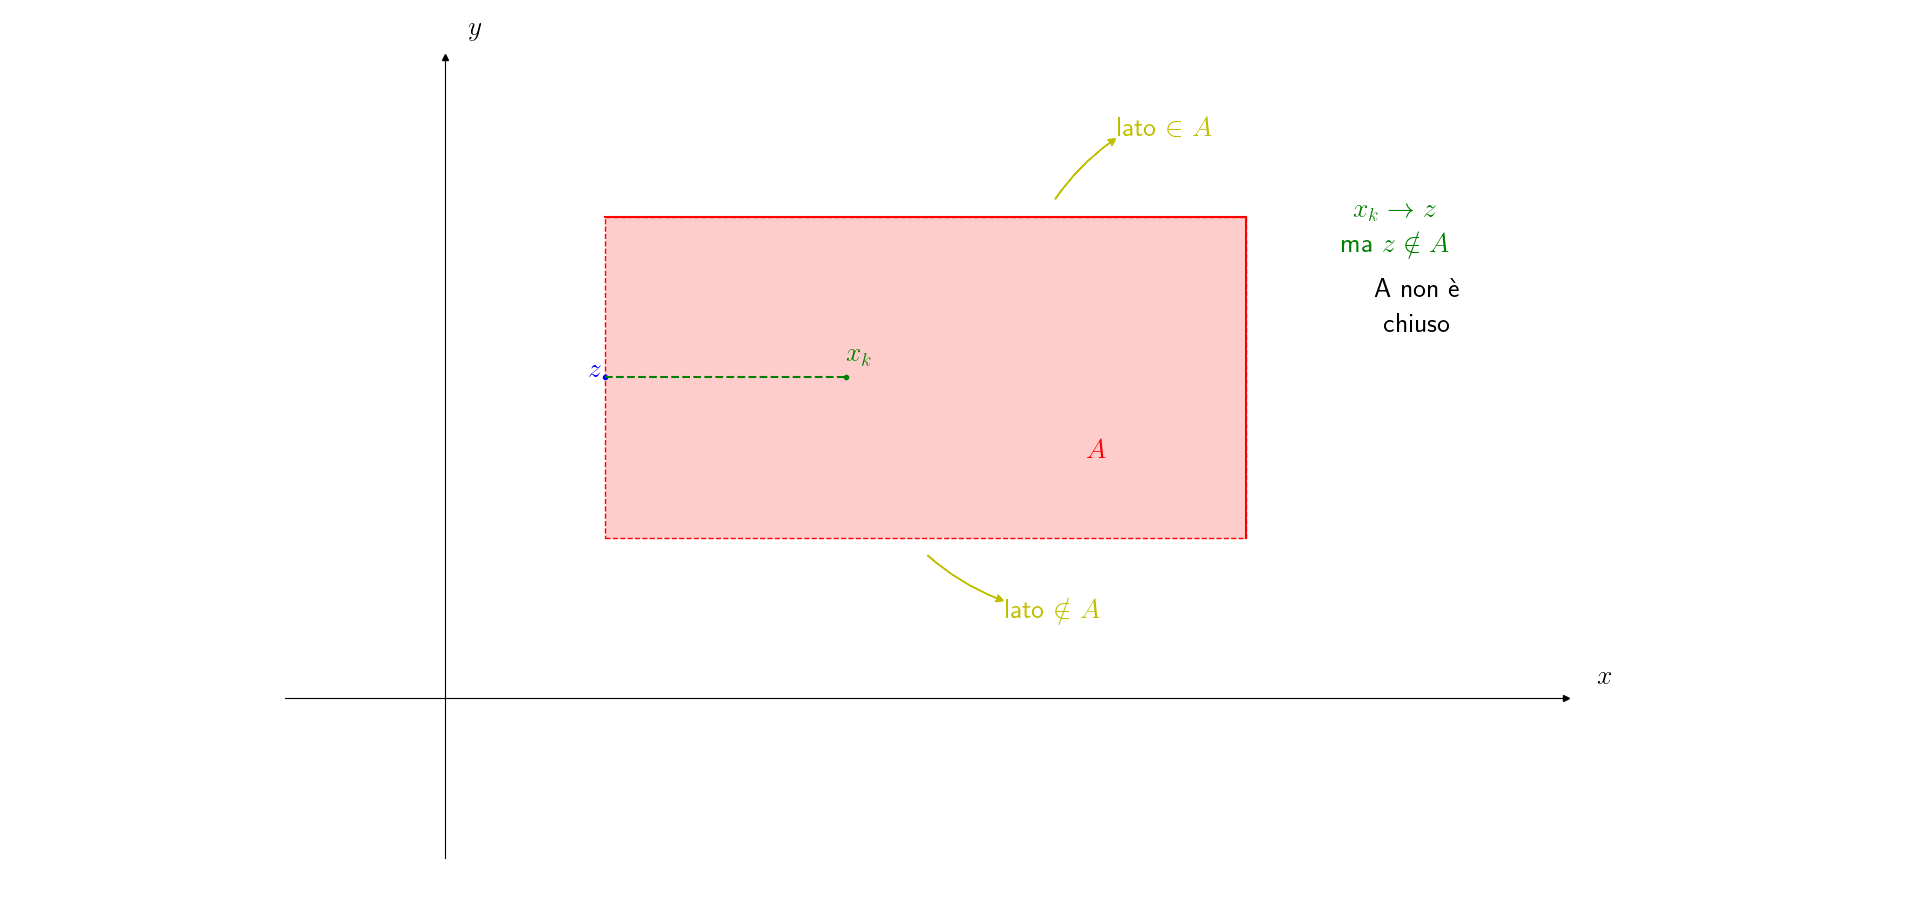
\includegraphics[width=0.75\linewidth]{spazi_metrici_e_normati/pag159}
		\label{fig:pag159}
	\end{center}	
\end{exbar}


\begin{exbar}
\begin{example} \textbf{importante}
	
	$C \subseteq \mathbb{R}^n$. Sono equivalenti le seguenti affermazioni
	\begin{enumerate}
		\item $C$ è chiuso per la topologia data dalla norma euclidea $|\cdot|$
		
		\item $C$ è chiuso per la topologia data dalla norma $\parallel \cdot \parallel_\infty$
		
		\item $C$ è chiuso per la topologia data dalla norma $\parallel \cdot \parallel_1$
	\end{enumerate}
	
	Per dimostrare che le tre affermazioni sono equivalenti, partiamo da
	\begin{gather*}
		|x_j| \leq |\overline{x}| \leq \sum_{i=1}^{n} |x_i| \qquad \forall \ \overline{x} = (x_1, \ldots, x_n) \in \mathbb{R}^n
		\\
		\lowercomment{\max_{j = 1, \ldots, n} |x_j|} {= \parallel \overline{x} \parallel_\infty} {}
		\leq |\overline{x}| \leq 
		\lowercomment{\sum_{i=1}^{n} |x_i|} {= \parallel \overline{x} \parallel_1} {} 
		\leq n \lowercomment{\max_{j = 1, \ldots, n} |x_j|} {= \parallel \overline{x} \parallel_\infty} {}
		\\
		\parallel \overline{x} \parallel_\infty \leq |\overline{x}| \leq \parallel \overline{x} \parallel_1 \leq n \parallel \overline{x} \parallel_\infty \qquad \forall \ \overline{x} \in \mathbb{R}^n
	\end{gather*}
	
	\begin{itemize}
		\item $1) \Rightarrow 2)$ 
		
		Ipotesi: $C$ è chiuso per $|\cdot|$. 
		
		Tesi: $C$ è chiuso per $ \parallel \cdot \parallel_\infty$
		
		$\{ \overline{x_k} \}_{k\geq 1} \subseteq C \ \big| \ \overline{x_k} \rightarrow \overline{z}$ per $\parallel \cdot \parallel_\infty$, cioè $\parallel \overline{x_k} - \overline{z} \parallel_\infty \rightarrow 0 $ per $k \rightarrow +\infty$, e dimostriamo che $\overline{z} \in C$
		\begin{equation*}
			|\overline{x_k} - \overline{z}| \lowercomment{\leq} {\text{disuguaglianza sopra}} {\text{con } \overline{x} = \overline{x_k} - \overline{z}}
			n \parallel \overline{x_k}-\overline{z} \parallel_\infty \rightarrow 0
		\end{equation*}
		
		$\Rightarrow |\overline{x_k} - \overline{z}| \rightarrow 0$ per $k \rightarrow +\infty$, cioè $\overline{x_k} \rightarrow \overline{z}$ per $|\cdot|$. Ma $C$ è chiuso per $|\cdot| \Rightarrow \overline{z} \in \mathbb{C}$.
		
		\item $2) \Rightarrow 3)$
		
		Ipotesi: $C$ è chiuso per $\parallel \cdot \parallel_\infty$.
		
		Tesi: $C$ è chiuso per $\parallel \cdot \parallel_1$
		
		$\{ \overline{x_k} \}_{k \geq 1} \subseteq C \ \big| \ \overline{x_k} \rightarrow \overline{z}$ per $\parallel \cdot \parallel_1$, cioè $\parallel \overline{x_k} - \overline{z} \parallel_1 \rightarrow 0$ per $k \rightarrow +\infty$ e dimostriamo che $\overline{z} \in C$.
		\begin{equation*}
			\parallel \overline{x} \parallel_\infty \leq \parallel \overline{x} \parallel_1 \qquad \forall \ \overline{x}\in \mathbb{R}^n
		\end{equation*}

		Prendo $\overline{x} = \overline{x_k} -\overline{z}$
		
		\begin{gather*}
			\parallel \overline{x_k} - \overline{z} \parallel_\infty \leq  \parallel \overline{x_k} -\overline{z} \parallel_1 \rightarrow 0 \Rightarrow \overline{x_k}  \rightarrow \overline{z} \text{ per } \parallel \cdot \parallel_\infty \rightarrow \overline{z} \in \mathbb{C}
		\end{gather*}
	
		perché $C $ è chiuso  per $\parallel \cdot \parallel_\infty$.
		
		\item $3) \Rightarrow 1)$ 
		
		Ipotesi: $C$ è chiuso per $\parallel \cdot \parallel_1$. 
		
		Tesi: $C$ è chiuso per $|\cdot|$
		
		$\{ \overline{x_k}\}_{k \geq 1} \subseteq C \ \big| \ \overline{x_k} \rightarrow \overline{z}$ per $|\cdot|$ e dimostriamo che $\overline{z} \in C$ 
		\begin{gather*}
			\parallel \overline{x} \parallel_1 \leq n \parallel \overline{x} \parallel_\infty \qquad \forall \ \overline{x} \in \mathbb{R}^n
			\\
			\frac{1}{n} \parallel \overline{x} \parallel_1 \leq \parallel \overline{x}\parallel_\infty \leq |\overline{x}| \qquad \forall \ \overline{x} \in \mathbb{R}^n
			\\
			\parallel \overline{x} \parallel_1 \leq n |\overline{x}| \qquad \forall \ \overline{x} \in \mathbb{R}^n
			\\
			\overline{x} = \overline{x_k} - \overline{z}
			\\
			\Rightarrow \parallel \overline{x_k} - \overline{z} \parallel_1 \leq n |\overline{x_k} - \overline{z}| \rightarrow 0 \text{ per } k \rightarrow +\infty
			\\
			\Rightarrow \parallel \overline{x_k} - \overline{z} \parallel_1 \rightarrow 0 \text{ per } k \rightarrow +\infty
			\\
			\Rightarrow \overline{x_k} - \overline{z} \text{ per } \parallel \cdot \parallel_1 \Rightarrow z \in C
		\end{gather*}
		
		perché $C$ è chiuso per $\parallel \cdot \parallel_1$.
	\end{itemize}
\end{example}
\end{exbar}


\textbf{Osservazione:}

Siccome $C$ è chiuso $\iff C^c$ è aperto, il corollario al teorema che abbiamo appena dimostrato implica che $A \subseteq R^n$ è aperto per $|\cdot|  \iff A $ è aperto per la topologia data da $\parallel \cdot \parallel_\infty \iff A$ è aperto per $\parallel \cdot \parallel_1$, cioè le 3 norme $|\cdot|$, $\parallel \cdot \parallel_\infty$, $\parallel \cdot \parallel_1$ descrivono la stessa topologia.

\begin{attbar}
	Si può dimostrare che in $\mathbb{R}^n$ (spazio di dimensione finita) tutte le norme sono equivalenti, cioè se $A \subseteq \mathbb{R}^n$ è aperto per una norma, lo è per qualsiasi altro.
\end{attbar}


\begin{definition}
	$(X,d)$ spazio metrico. $K \subseteq X$ si dice limitato se $\exists \ x \in X$ e $R>0 \ \big|$ $K \subseteq B_R(x)$, cioè $d(x,z) < R \quad \forall \ z \in K$. 
\end{definition}


\begin{exbar}
	$K \subseteq \mathbb{R}$ è limitato se $\exists R > 0 \ \big| \ K \subseteq \ ]-R, R \ [ \ = B_R(0)$ cioè $|z| < R \quad \forall \ z \in K$.
\end{exbar}


\textbf{Osservazione:}
Se $(X, \parallel \cdot \parallel)$ è spazio normato, il punto $x \in X$ nella definizione di insieme limite può essere preso coincidente con $0$. 

Infatti se $k \subseteq B_R(x)$
\begin{gather*}
	\Rightarrow \lowercomment{ \parallel x-z \parallel} {= d(x,z)} {} < R \qquad \forall \ z \in K
	\\
	z \in K \qquad \parallel z \parallel = \parallel z - x + x \parallel \distr \parallel x-z \parallel + \parallel x\parallel < R + \parallel x \parallel 
	\\
	\Rightarrow z \in B_{R + \parallel x \parallel}(0)
\end{gather*}

Quindi, in uno spazio normato, $K \subseteq X$ è limitato se $\exists \ R >0 \ \big| \ K \subseteq B_R(0)$, cioè $\parallel z \parallel < R$ $\forall \ z \in K$. 

(se $x = R$ e $\parallel \cdot \parallel = |\cdot|$, si ritrova quanto scritto sopra.)


\begin{proposition}

	$(X,d)$ spazio metrico. $\{ x_k \}_{k\geq 1} \subseteq X$ successione convergente. Allora $\{ x_k \}_{k \geq 1}$ è limitata, cioè $\exists x \in X$ e $R >0 \ \big| \ x_k \in B_R(x) \quad \forall \ k \geq 1$
	
	$(d(x_k,x)< R \quad \forall \ k \geq 1)$
\end{proposition}


\begin{exbar}
\begin{example}
	$C^0 ([0,1])$
	
	$K = \{ f \in C^0 ([0,1]) \ \big| \ |f(x)| \leq \frac{1}{\sqrt{x}} \qquad \forall x \in \ ]0,1] \}$
	\begin{itemize}
		\item $(C^0 ([0,1]), \parallel \cdot \parallel_1)$, $K$ è limitato 
		\begin{gather*}
			f \in K \qquad \parallel f \parallel_1 = \int_{0}^{1} |f(x)| \ \mathrm{d}x \leq \int_{0}^{1} \frac{1}{\sqrt{x}} \ \mathrm{d}x = \lim_{c \rightarrow 0^+} \int_{c}^{1} \frac{1}{\sqrt{x}} \ \mathrm{d}x = 2
			\\
			\parallel f \parallel_1 \leq 2 \qquad \forall \ f \in K
			\\
			K \subseteq \overline{B_{2}^{\parallel \cdot \parallel_1}(0)} \subseteq B_{3}^{\parallel \cdot \parallel_1}(0)
		\end{gather*}

		\item ($C^0 ([0,1]), \parallel \cdot \parallel_\infty$), $K$ è illimitato
		
		\begin{center}
			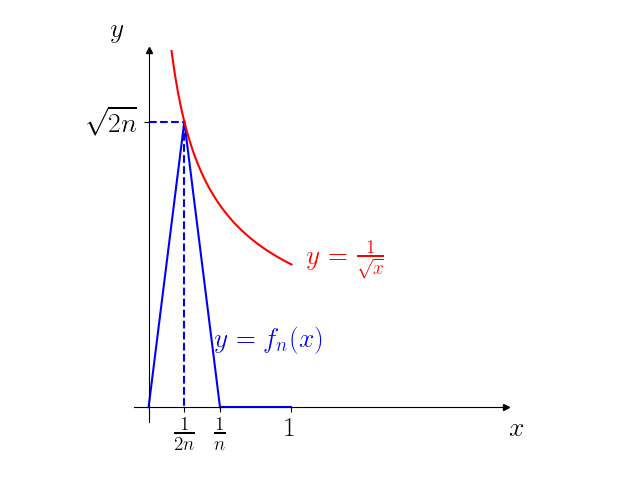
\includegraphics[width=0.7\linewidth]{spazi_metrici_e_normati/pag165}
			\label{fig:pag165}
		\end{center}
		
		$\parallel f_n \parallel_\infty = \sqrt{2n} \rightarrow +\infty \text{ se } n \rightarrow +\infty, \quad f_n \in K$
		
		\item $C^0 ([0,1]), \{ f_n \}_{n \geq 1}$ come sopra. Allora $f_n \rightarrow f = 0$ per $\parallel \cdot \parallel_1$
		\begin{gather*}
			\parallel f_n - 0 \parallel_1 =\int_{0}^{1} |f(x)| \mathrm{d}x = \frac{1}{n} \ \sqrt{2n} \ \frac{1}{2} = \frac{1}{\sqrt{2n}} \rightarrow 0 \textbf{ per } n \rightarrow +\infty
			\\
			\text{Ma } \parallel f_n - 0 \parallel_\infty = \sqrt{2n} \rightarrow +\infty \Rightarrow f_n \nrightarrow 0 \text{ per } \parallel \cdot \parallel_\infty
		\end{gather*}
	\end{itemize}
\end{example}
\end{exbar}


\textbf{Osservazione:}
$K \subseteq \mathbb{R}^n$ è limitato per $|\cdot| \iff$ lo è per $\parallel \cdot \parallel_\infty \iff$ lo è per $\parallel \cdot \parallel_1$
\begin{equation*}
	\parallel \overline{x} \parallel_\infty \leq |\overline{x}| \leq \parallel \overline{x} \parallel_1 \leq n \parallel \overline{x} \parallel_\infty
\end{equation*}


\begin{center}
	\label{fig:pag166_1}
	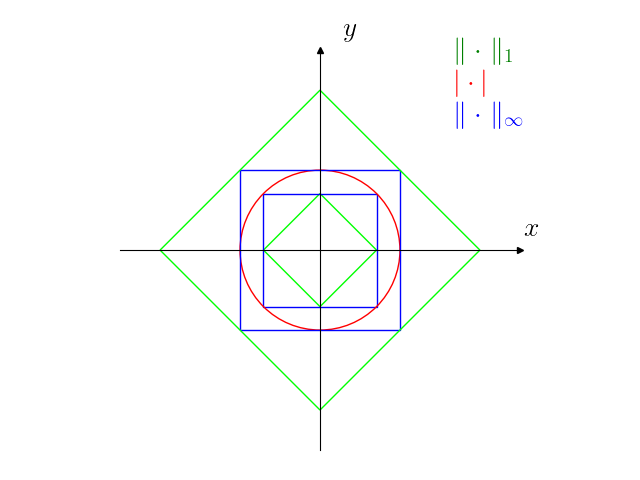
\includegraphics[width=0.7\linewidth]{spazi_metrici_e_normati/pag166_1}
\end{center}


\textbf{Osservazione:}
Introduciamo in $\mathbb{R}^n$ il simbolo $\infty$. Un intorno di $\infty$ è un qualunque insieme $A \subseteq \mathbb{R}^n \; \big| \; A$ contiene il complementare di una palla di centro l'origine, cioè $\exists \ R > 0 \; \big| \; \overline{x} \in A$ $\Rightarrow \parallel \overline{x} \parallel > R$
\begin{center}
	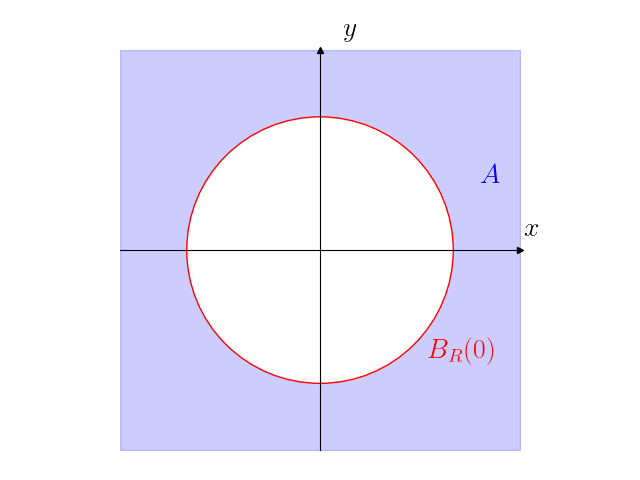
\includegraphics[width=0.7\linewidth]{spazi_metrici_e_normati/pag166_2}
	\label{fig:pag1662}
\end{center}

Una successione $\{\overline{x_k}\}_{k \geq 1} \subseteq \mathbb{R}^n$ si dice divergente a $\infty$ e si scrive $\lim_{k} \overline{x_k} = \infty$ se $\lim_{k} |\overline{x_k}| = +\infty$ cioè se $\forall \ R > 0 \; \exists \ N > 0 \; \big| \; k > N \Rightarrow |\overline{x_k}| > R$


\begin{exbar}
\begin{example}
\begin{gather*}
\overline{x_k} = (\lowercomment{e^{-k}} {x_{k1}} {}, \lowercomment{2+\frac{1}{k}} {x_{k2}} {}, \lowercomment{\ln k} {x_{k3}} {}) \subseteq \mathbb{R}^3, \qquad k \geq 1
\\
\lim_{k} x_{k1} = \lim_{k} e^{-k} = 0
\\
\lim_{k} x_{k2} = \lim_{k} 2 + \frac{1}{k} = 2
\\
\lim_{k} x_{k3} = \lim_{k} \ln k = +\infty
\\
\lim_{k} |\overline{x_k}| = \lim_{k} \sqrt{e^{-2k} + \bigg(2+\frac{1}{k} \bigg)^2 + (\ln k)^2} = +\infty \Rightarrow \lim_{k} \overline{x_k} = \infty
\end{gather*}
\end{example}
\end{exbar}


\subsection{Limiti di funzione}
\begin{definition}
	$(X,d)$ spazio metrico, $A \subseteq X$, non vuoto. $x_0 \in X$ si dice \textbf{punto di accumulazione} per $A$ se  $\forall \epsilon >0 \ \exists \ x \in A, x \neq x_0,$ tale che $x \in B_\epsilon(x_0)$, cioè se $B_\epsilon (x_0) \cap A$ contiene punti di $A$ diversi da $x_0$. 
	
	$x_0 \in A$ si dice \textbf{punto isolato} se non è di accumulazione, cioè se $\exists \epsilon > 0$ tale che \\ %riq malf
	$B_\epsilon (x_0) \ \cap \ A =\{ x_0 \}$.
\end{definition}


\begin{definition}
	$(X,d_x),(Y,d_y)$ spazi metrici, $f:dom \ f \rightarrow Y$, con $dom \ f \subseteq X, x_0 \in X $ punto di accumulazione per $dom \ f$. Si dice che $f$ ha limite $\ell \in Y$ per $x \rightarrow x_0$ e si scrive
	\begin{equation*}
	\begin{array}{r l}
		\lim_{x \rightarrow x_0} f(x) = \ell & \text{oppure}
		\\
		f(x) \rightarrow \ell & \text{per } x \rightarrow x_0
	\end{array}
	\end{equation*}
	se per ogni intorno  $V$ di $\ell$  esiste un intorno $U$ di $x_0 \; \big| \; f(x) \in V, \ x \in U \cap dom \ f, x \neq x_0 $
	
	In altre parole, $\lim_{x \rightarrow x_0} f(x) = \ell \quad \forall \epsilon > 0 \quad \exists \ \delta > 0 \; \big| $ se $ 0 < \lowercomment{d_x(x, x_0)} {x \in B_\delta^x(x_0)} {} < \delta$ e $x \in dom \ f $, allora $\lowercomment{d_y (f(x), \ell)} {f(x) \in B_\epsilon^y(\ell)} {} < \epsilon$ 
	
	(Se prendo la definizione data con $\epsilon$ e $\delta$ per $X = Y = \mathbb{R}$ e le distanze \\ %riq malf
	$d_x(x,y) = d_y(x,y) = |x-y|$, ottengo la definizione con $\epsilon$ e $\delta$ data in ambito reale.)
\end{definition}


\begin{theorem} (di unicità del limite)
	
	$(X,d_x)$ e $(Y,d_y)$ spazi metrici, $f : dom \ f \rightarrow Y, \ dom \ f \subseteq X, \ x_0 \in X$ punto di accumulazione per $dom \ f$.
	
	Se $\lim_{x \rightarrow x_0} f(x) = \ell_1 \in Y$ e $\lim_{x \rightarrow x_0} f(x) = \ell_2 \in Y$, allora $\ell_1 = \ell_2$.
\end{theorem}


\begin{proposition}
	$(X,d)$ spazio metrico, $\overline{f}: dom \ \overline{f} \rightarrow \mathbb{R}^n,\; \overline{f}(x) = \big(f_1(x), \ldots, f_n(x) \big), \ x_0 \in X$ punto di accumulazione per $dom \ \overline{f} \subseteq X$, allora 
	\begin{equation*}
		\lim_{x \rightarrow x_0} \overline{f}(x) = \overline{\ell} = (\ell_1, \ldots, \ell_n) \in \mathbb{R}^n \iff \lim_{x \rightarrow x_0} f_j(x) = \ell_j \qquad \forall j = 1, 2, \ldots, n
	\end{equation*}
\end{proposition}


\begin{theorem} (della permanenza del segno)
	
	$(X,d)$ spazio metrico, $f: dom \ f \rightarrow \mathbb{R}, \ dom \ f \subseteq X, \ x_0 \in X$ punto di accumulazione per $dom \ f$.
	
	Se $\lim_{x \rightarrow x_0} f(x) = \ell > 0$, allora $f(x) > 0$ definitivamente per $ x \rightarrow x_0$, cioè $\exists \ \delta > 0 \; \big| \; f(x) > 0$ $\forall \ x \in B_\delta (x_0) \cap dom \ f, \ x \neq x_0$. 
\end{theorem}


\begin{theorem}
	$(X,d)$ spazio metrico, $f,g: A \rightarrow \mathbb{R}, \ A \subseteq X, \ x_0 \in X$ punto di accumulazione per $A$, tali che $\lim_{x \rightarrow x_0} f(x) = \ell_f, \ \lim_{x \rightarrow x_0} g(x) = \ell_f$ e $f(x) \leq g(x)$ definitivamente per $x \rightarrow x_0$. ($\exists \ \delta > 0 \; \big| \; f(x) \leq g(x) \forall x \in B_\delta (x_0) \cap A$, \ $x \neq x_0$.)
	
	Allora $\ell_f \leq \ell_g$.
\end{theorem}


\begin{theorem}(del confronto o dei due carabinieri)
	
	$(X,d)$ spazio metrico, $f,g,h : A \rightarrow \mathbb{R}, \ A \subseteq X, x_0$ punto di accumulazione per $A$, tali che $g(x) \leq f(x) \leq h(x)$ definitivamente per $x \rightarrow x_0$. 
	
	Se $\lim_{x \rightarrow x_0} g(x) = \lim_{x \rightarrow x_0} h(x) = \ell$, allora $\lim_{x \rightarrow x_0} f(x) = \ell$.
\end{theorem}


\subsection{Funzioni continue tra spazi metrici}

\begin{definition}	
	$(X,d_x), \ (Y,d_y)$ spazi metrici, $f:dom \ f \rightarrow Y, \ dom \ f \subseteq X$, si dice \textbf{continua in } $\mathbf{x_0 \in dom \ f}$ se vale una delle due
	\begin{enumerate}
		\item $x_0$ è punto isolato per $dom \ f$
		\item $\lim_{x \rightarrow x_0} f(x) = f(x_0)$
	\end{enumerate}
	
	In altre parole, $f$ è continua in $x_0$ se $\forall \ \epsilon > 0 \ \exists \ \delta > 0 \; \big| \; \text{ se } d_x(x, x_0) < \delta \text{ e } x \in dom \ f$, allora $d_y(f(x), f(x_0) < \epsilon$. 
	

	$\bigg( \begin{array}{l}
	x \in B_{\delta}^{x}(x_0) \cap dom \ f \Rightarrow f(x) \in B_{\epsilon}^{y} (f(x_0)) \Rightarrow x \in f^{-1}(B_{\epsilon}^{y} (f(x_0))
	\\
	\forall \ \epsilon > 0 \ \exists \ \delta > 0 \; \big| \; B_{\delta}^{x}(x_0) \cap dom \ f \subseteq f^{-1} (B_{\epsilon}^{y} (f(x_0)))
	\end{array}
	\bigg)$
	
	Una funzione $f:dom \ f \rightarrow Y $ si dice continua se è continua in ogni punto del suo dominio.
\end{definition}


\begin{theorem}
	\label{th: pag172}
	$(X,d_x), \ (Y,d_y)$ spazi metrici, $f:X \rightarrow Y$. $f$ è continua $\iff f^{-1}(A)$ è aperto (in $X$) per ogni aperto $A \subseteq Y$.
\end{theorem}


\begin{dembar}
\textbf{Dimostrazione} del \textbf{Teorema \ref{th: pag172}}

	
	\begin{itemize}
		\item $\Rightarrow)$ Ipotesi: $f$ continua.
		
		Tesi: Dato $A \subseteq Y$ aperto, $f^{-1}(A)\subseteq X$ è aperto.
		
		Sia $x_0 \in f^{-1}(A)$. Dobbiamo trovare una palla centrata in $x_0$ contenuta in $f^{-1}(A)$.
		
		$f(x_0) \in A$, che è aperto, 
		\begin{gather*}
			\exists \ \epsilon >0 \; \big| \; B_{\epsilon}^{Y} (f(x_0)) \subseteq A
			\\
			\exists \ \delta > 0 \; \big| \; B_{\delta}^{X} (x_0) \Rightarrow f(x) \in B_{\epsilon}^{Y} (f(x_0)) \subseteq A
			\\
			B_{\delta}^{X}(x_0) \subseteq f^{x_0} (A) \text{, come si voleva.}
		\end{gather*}
		\item $\Leftarrow)$ Ipotesi: $f^{-1}(A) \subseteq X$ è aperto $\forall A \subseteq Y$ aperto. Tesi: $f$ è continua
		
		Fissiamo $x_0 \in X$ e $\epsilon > 0$.
		
		Dobbiamo trovare $\delta > 0 \; \big| \; x \in B_{\delta}^{X} (x_0) \Rightarrow f(x) \in B_{\epsilon}^{Y} (f(x_0))$
		
		\begin{gather*}
			B_{\epsilon}^{y} (f(x_0)) \text{ è un aperto } \Rightarrow f^{-1}(B_{\epsilon}^{Y} (f(x_0))) \text{ è aperto e } x_0 \in f^{-1} (B_{\epsilon}^{Y} (f(x_0))) 
			\\
			\Rightarrow \exists \ \delta > 0 \; \big| \; B_{\delta}^{X} (x_0) \subseteq f^{-1} (B_{\epsilon}^{Y}(f(x_0))) 
			\\
			\text{ cioè, se } x \in B_{\delta}^{X}(x_0) \Rightarrow f(x) \in B_{\epsilon}^{Y} (f(x_0)) \text{ come si voleva.} \qquad \square
		\end{gather*}
		
	\begin{center}
		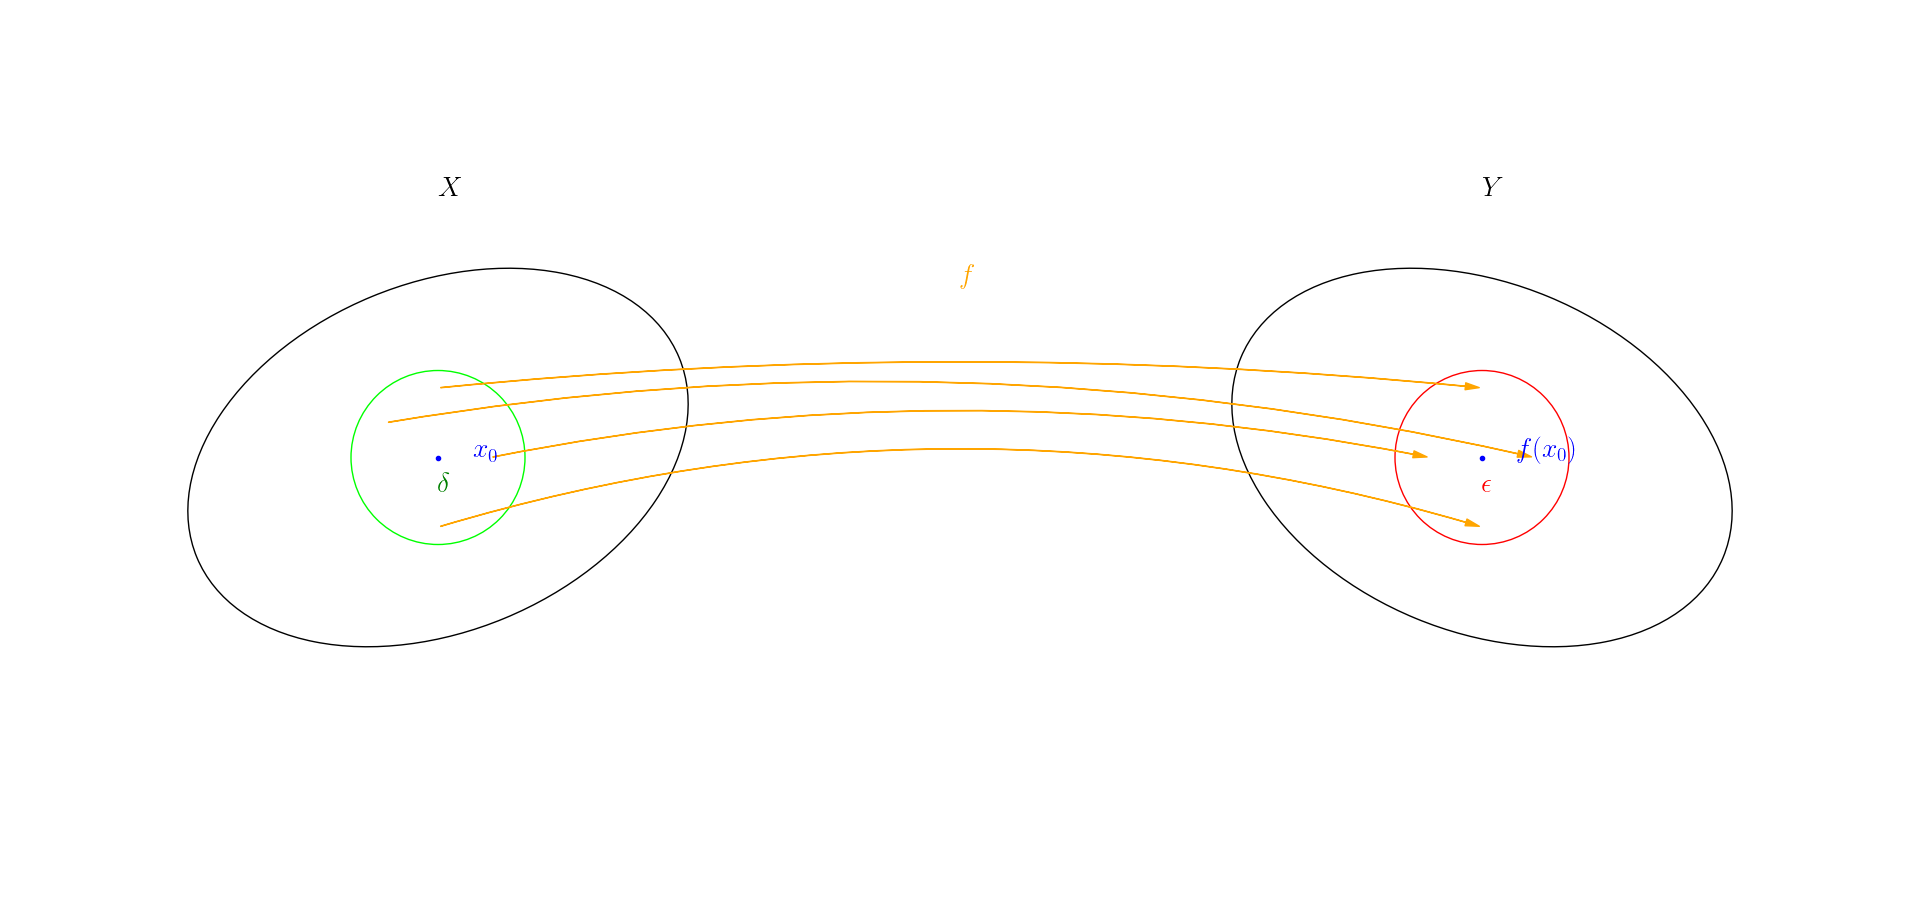
\includegraphics[width=0.7\linewidth]{spazi_metrici_e_normati/pag174}
		\label{fig:pag174}
	\end{center}
	\end{itemize}
\end{dembar}


\begin{theorem}
	$(X,d)$ spazio metrico. $A \subseteq X, \ f,g: A \rightarrow \mathbb{R}, \ x_0 \in A$, $f$ e $g$ continue in $x_0$. Allora $f + g, f \cdot g$ e $f / g$, se $g(x_0) \neq 0$, sono continue in $x_0$.
\end{theorem}


\begin{proposition}
	$(X,d)$ spazio metrico, $A \subseteq X, \overline{f}: A \rightarrow \mathbb{R}^n, \ \overline{f}(x) = (f_1(x), \ldots, f_n(x))$, è continua in $x_0 \in A \iff$ sono continue in $x_0$ le sue componenti $f_j \qquad \forall j = 1, \ldots, n$.
\end{proposition}


\begin{exbar}
\begin{example}
	$(X,d_x),(Y,d_y)$ spazi metrici.
	\begin{enumerate}
		\item Provare che \begin{gather*}
			d((x_1,y_1), (x_2,y_2)) = \sqrt{(d_x(x_1,x_2))^2 + (d_y(y_1,y_2))^2}
			\\
			(x_1, y_1), (x_2,y_2) \in X \times Y \text{ è una metrica in } X \times Y
		\end{gather*}
		
		\item Provare che $\forall r > 0$ vale
		\begin{equation*}
			B_{\frac{r}{\sqrt{2}}}^{X}(x) \times B_{\frac{r}{\sqrt{2}}}^{Y}(y) \subseteq B_{r}^{X \times Y} ((x_0,y_0)) \subseteq B_{r}^{X} (x_0) \times B_{r}^{Y} (y_0)
		\end{equation*}
		
		\begin{center}
			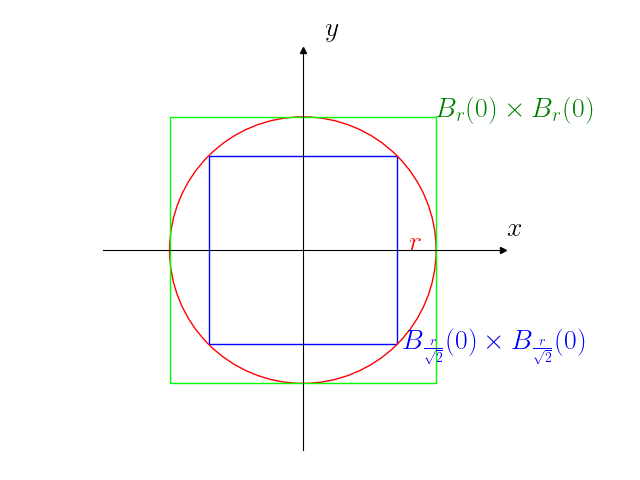
\includegraphics[width=0.7\linewidth]{spazi_metrici_e_normati/pag175}
			\label{fig:pag175}
		\end{center}
			
		\item Sia ora $Y = \mathbb{R}$ con la metrica usuale che deriva dal valore assoluto.
		
		$f:X \rightarrow \mathbb{R}$
		
		$A = \{ (x,y) \in X \times \mathbb{R} \; \big| \; y > f(x) \}$
		
		$C = \{ (x,y) \in X \times \mathbb{R} \; \big| \; y \geq f(x) \}$
		
		Provare che, se $f $ è continua, allora $A$ è aperto e $C$ è chiuso in $X \times \mathbb{R}$ con la metrica $d$.
		
		\item Provare che, in generale, il viceversa non è vero, cioè $A$ può essere aperto con $f$ discontinua e $C$ chiuso con $f$ discontinua.	
	\end{enumerate}

	\begin{center}
		$\sim \circ \sim$
	\end{center}

	\begin{enumerate}
		\item Per casa
		
		\item Facciamo vedere che se $(x,y) \in B_{\frac{r}{\sqrt{2}}}^{X}(x_0) \times B_{\frac{r}{\sqrt{2}}}^{Y}(y_0)$, allora $(x, y) \in B_{r}^{X \times Y} ((x_0, y_0))$
		
		\begin{equation*}
			d_x(x, x_0) < \frac{r}{\sqrt{2}} \text{  e  } d_y(y, y_0) < \frac{r}{\sqrt{2}}
			\Rightarrow d((x,y), (x_0,y_0)) < r
		\end{equation*}
		\begin{align*}
			d((x,y),(x_0,y_0)) 
			&= \sqrt{(d_x(x, x_0))^2 + (d_y(y,y_0))^2} <
			\\
			&< \sqrt{\left( \frac{r}{\sqrt{2}} \right)^2+\left( \frac{r}{\sqrt{2}} \right)^2} = \sqrt{r^2} = r
		\end{align*}

		Facciamo vedere che, se $(x,y) \in B_{r}^{X \times Y}((x_0, y_0))$, allora $(x,y) \in B_{r}^{X} (x_0) \times B_{r}^{Y} (y_0)$, cioè che, se $d((x,y), (x_0,y_0)) < r$, allora $d_x(x, x_0) < r$ e $d_y(y, y_0) < r$
		
		\begin{equation*}
			d_x (x, x_0)= \sqrt{(d_x (x, x_0))^2} \leq \sqrt{(d_x (x, x_0))^2 + (d_y (y, y_0))^2} = d((x,y), (x_0,y_0)) < r
		\end{equation*}
	
		\item Introduciamo la funzione 
		\begin{align*}
			\phi: 
			&X \times \uppercomment{\mathbb{R}} {} {\text{c'è la metrica } d} \rightarrow \mathbb{R},
			\\
			&(x,y) \mapsto y-f(x)
		\end{align*}
		\begin{gather*}
			A= \{ (x,y) \in X \times \mathbb{R} \; \big| \; \phi(x, y) > 0 \} = \phi^{-1} \big( ]0,+\infty[ \big)
			\\
			C = \{ (x,y) \in X \times \mathbb{R} \; \big| \; \phi(x, y) \geq 0 \} = \phi^{-1} \big( ]0,+\infty[ \big)
			\\
			\phi^{-1} \big( B^c \big) = \big( \phi^{-1}(B) \big)^c
			\\
			x \in \phi^{-1} \big( B^c \big) \iff \phi(x) \in B^c \iff \phi(x) \notin B \iff x \notin \phi^{-1} \big( B \big) \iff x \in \big( \phi^{-1}(B) \big)^c
		\end{gather*}

		Se $B$ è chiuso e $\phi$ è continua, 
		\begin{gather*}
			\phi^{-1} \big( B \big) = \phi^{-1}\big( (B^c)^c\big) =
			\\
			= \big( \lowercomment{\phi^{-1} (\lowercomment{B^c} {\text{aperto}} {}) } {\text{aperto}} {} \big)^c \text{ è chiuso}
		\end{gather*} 
		
		cioè l'antimmagine di un chiuso tramite una funzione continua è un insieme chiuso.
		
		Poiché $B = [0,+\infty[$ è chiuso e $C = \phi^{-1} \big( B \big)$, se $\phi$ è continua, $C$ è chiuso.
		
		Tutto l'esercizio si riduce a dimostrare che $\phi$ è continua.
		
		\begin{align*}
			\phi_1: 
			& X \times \mathbb{R} \rightarrow \mathbb{R},
			& \phi_2: 
			& X \times \mathbb{R} \rightarrow \mathbb{R}
			\\
			& (x,y) \mapsto y
			&
			& (x,y) \mapsto f(x)
		\end{align*}
		\begin{equation*}
			\phi(x,y) = \phi_1(x,y) - \phi_2(x,y)
		\end{equation*}
		
		Se dimostro che $\phi_1$ e $\phi_2$ sono continue, allora $\phi$ è continua perché differenza di funzioni continue.
		
		Dimostriamo la continuità di $\phi_1$.
		
		$(x_0, y_0) \in X \times \mathbb{R}$ e fissiamo $\epsilon > 0$
		
		Dobbiamo dimostrare che $\exists \ \delta > 0 \; \big| \; \text{ se } d((x,y), (x_0,y_0)) < \delta$, allora $\lowercomment{|y-y_0|}{| \phi_1(x, y) - \phi_2 (x_0, y_0) |}{} < \epsilon$
		
		Sia $U = X \times  ]y_0 - \epsilon, y_0 + \epsilon[$
		
		Se $(x,y) \in U \Rightarrow |\phi_1(x,y) - \phi_1(x_0,y_0)| = |y - y_0| < \epsilon$
		
		$U$ è un intorno di $(x_0, y_0)$, cioè
		\begin{gather*}
			\exists \ \delta > 0 \; \big| \; B_{\delta}^{X \times \mathbb{R}} ((x_0, y_0)) \subseteq U
			\\
			B_{\delta}^{X \times \mathbb{R}} ((x_0, y_0))\subseteq B_{\delta}^{X} (x_0) \times B_{\delta}^{\mathbb{R}} (y_0) \subseteq X \times ]y_0 - \epsilon, y_0 + \epsilon[
		\end{gather*}

		Continuità di $\phi_2$ in $(x_0,y_0)$
		
		$\forall \ \epsilon > 0$ devo trovare $\delta >0 \; | \; \text{ se } d((x,y), (x_0,y_0)) < \delta$ 
		\begin{equation*}
			\Rightarrow | \phi_2(x,y) - \phi_2(x_0,y_0)| = |f(x) - f(x_0)| < \epsilon
		\end{equation*}

		Poiché $f$ è continua, $\exists \ \delta > 0 \; \big| \; x \in B_{\delta}^{X} (x_0) \Rightarrow |f(x) - f(x_0)| < \epsilon$
		
		L'insieme $B_{\delta}^{X} (x_0) \times \mathbb{R}$ è un intorno di $(x_0,y_0)$ e $\forall \ (x,y) \in B_{\delta}^{X} (x_0) \times \mathbb{R}$ si ha
		\begin{equation*}
			|\phi_2(x,y) - \phi(x_0,y_0)| = |f(x) - f(x_0)| < \epsilon
		\end{equation*}
		
		\item $X = Y = \mathbb{R}$ con la distanza data dal valore assoluto
		
		\begin{equation*}
			f(x) = \lowercomment{\chi_{[0,+\infty[}(x)} {\text{funzione caratteristica di }[0,+\infty[}{\text{o funzione di Heaviside}} =
			\begin{cases}
				1 & \text{se } x \geq 0
				\\
				0 &  \text{se } x < 0
			\end{cases}
		\end{equation*}
		
		\begin{center}
			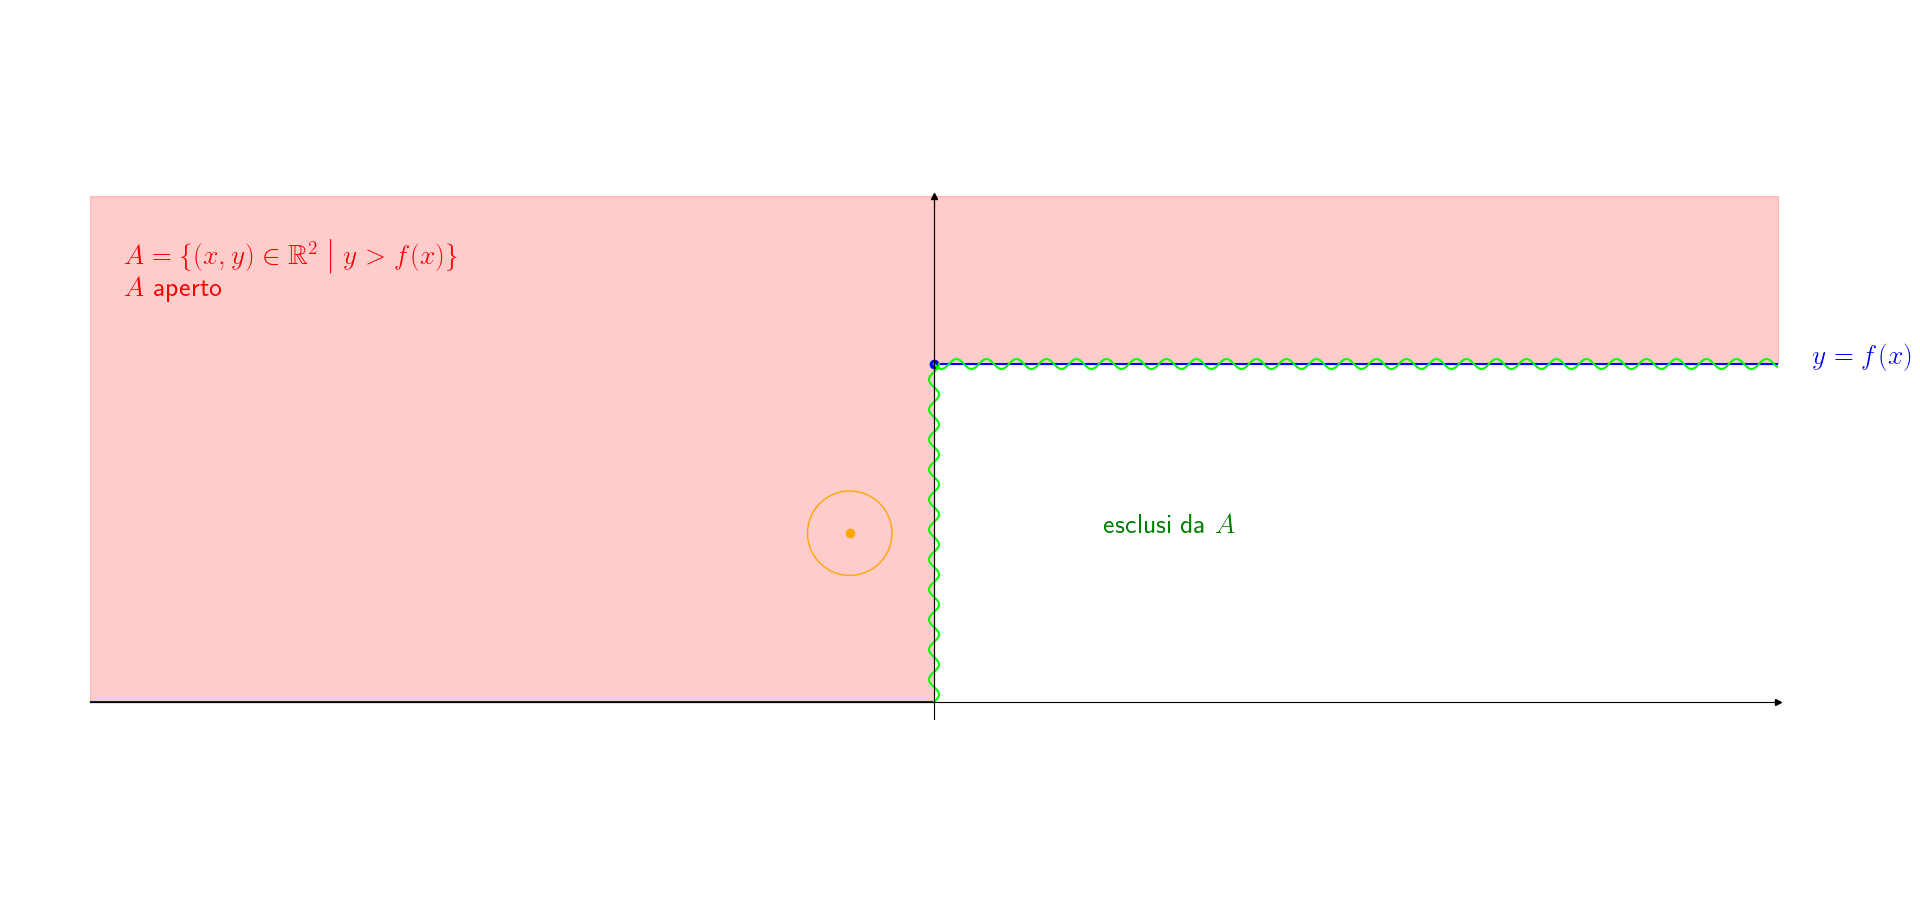
\includegraphics[width=0.7\linewidth]{spazi_metrici_e_normati/pag181_1}
			\label{fig:pag1811}
		\end{center}
		
		\begin{equation*}
			f(x) = 		\chi_{]0,+\infty[} = 
			\begin{cases}
				1 & \text{se } x > 0
				\\
				0 &  \text{se } x \leq 0
			\end{cases}
		\end{equation*}
		
		\begin{center}
			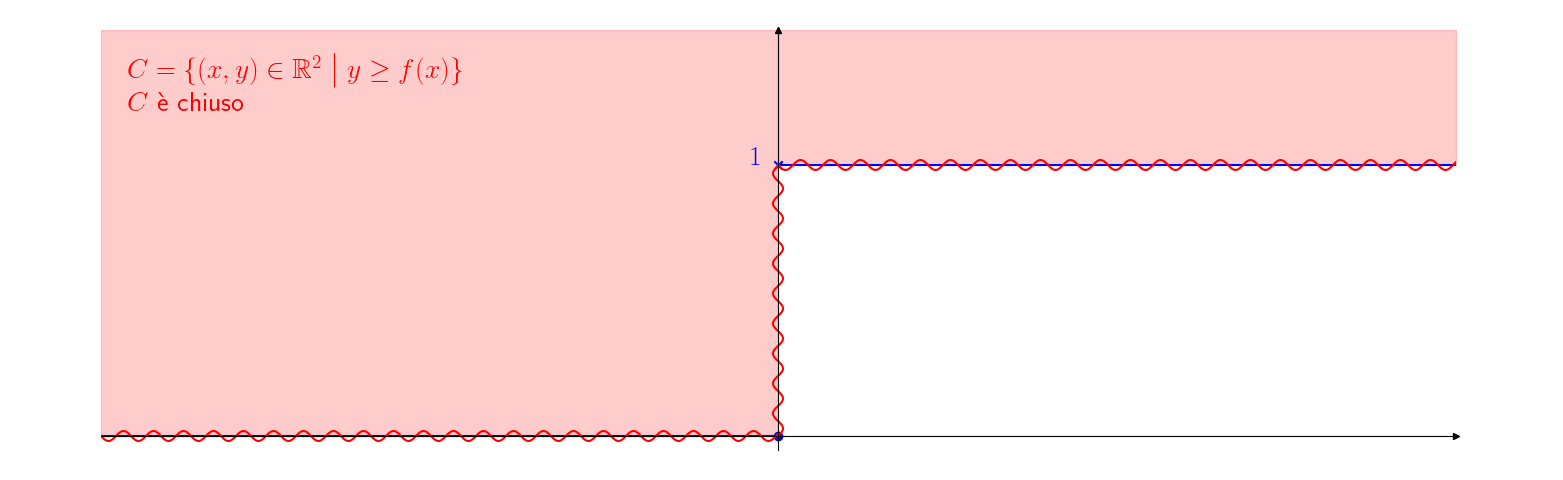
\includegraphics[width=0.7\linewidth]{spazi_metrici_e_normati/pag181_2}
			\label{fig:pag1812}
		\end{center}
	\end{enumerate}
\end{example}
\end{exbar}


\subsection{Successioni di funzioni}

\begin{definition}
	$(X,d)$ spazio metrico.
	
	Una successione di funzioni da $X$ in $\mathbb{R}$ è una funzione che ad ogni numero naturale $k$ associa una ed una sola funzione $f_k : X \rightarrow \mathbb{R}$. 
\end{definition}


\begin{definition}
	Sia $\{ f_k \}_{k \in \mathbb{N}}, f_k : X \rightarrow \mathbb{R}$, successione di funzioni. Si dice che la successione \textbf{converge puntualmente} in $D \subseteq X$ se $\{ f_k(x) \}_{k \in \mathbb{N}}$ converge $\forall \ x \in D$, cioè se $\forall \ x \in D$ esiste finito
	\begin{equation*}
		\lim_{k \rightarrow + \infty} f_k(x) = f(x),
	\end{equation*}
	limite puntuale della successione $f : D \rightarrow \mathbb{R}$. L'insieme degli $x \in X$ dove $\{f_k \}_{k \in \mathbb{N}}$ converge puntualmente si dice \textbf{insieme di convergenza puntuale} della successione.
\end{definition}


\begin{exbar}
	\begin{gather*}
	f_k: \mathbb{R} \rightarrow \mathbb{R}, \qquad f_k(x) = x^k
	\\
	\lim_{k \rightarrow + \infty} f_k(x) = \lim_{k \rightarrow + \infty} x^k =
	\begin{cases}
		0 & \text{se } |x|<1
		\\
		1 & \text{se } x=1 
		\\
		\nexists & \text{se } x \leq -1
		\\
		+\infty & \text{se } x >1
	\end{cases}
	\end{gather*}
	
	Insieme di convergenza puntuale: $D = ]-1,1]$
	
	Limite puntuale $f:D \rightarrow \mathbb{R}$		
	\begin{equation*} f(x) = \begin{cases}
		0 & \text{se } |x|<1
		\\
		1 & \text{se } x=1
	\end{cases}
	\end{equation*}	
\end{exbar}


\begin{definition}
	$f_k:X \rightarrow \mathbb{R}, k \in \mathbb{N}$, successione di funzione. Si dice che $\{ f_k \}_{k \in \mathbb{N} }$ \textbf{converge uniformemente} in $D \subseteq X$ ad una funzione $f: D \rightarrow \mathbb{R}$ se 
	\begin{gather*}
		\lim_{k \rightarrow +\infty} \sup_{x \in D} |f_k(x) - f(x)| = 0 
		\\
		\text{e si scrive } f_k \rightrightarrows f \text{ in } D
	\end{gather*}
	
	($\forall \epsilon >0 \exists N \; \big| \; k >N \quad \sup_{x \in D} |f_k(x)-f(x)| < \epsilon$, e quindi, in particolare $|f_k(x) - f(x)| < \epsilon$ $\forall \ x \in D$ cioè $f(x) - \epsilon <f_k(x) < f(x) + \epsilon \qquad \forall x \in D$)
	
	\begin{center}
		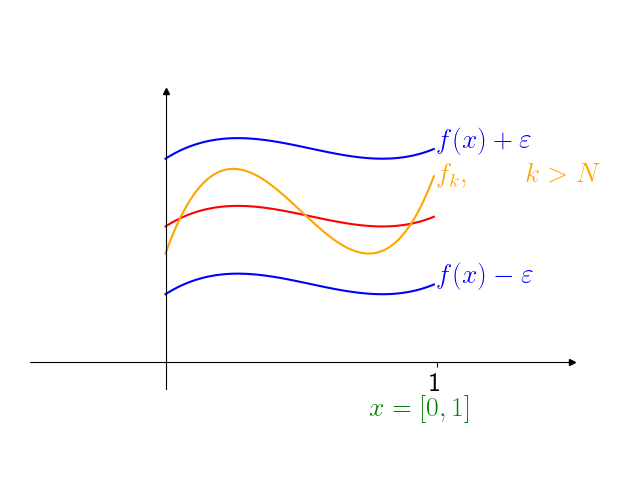
\includegraphics[width=0.7\linewidth]{spazi_metrici_e_normati/pag184}
		\label{fig:pag184}
	\end{center}
\end{definition}


\begin{exbar}
	$(X,d)$ spazio metrico
	
	$B(x) = \{ f:X \rightarrow \mathbb{R} \; \big| \; \lowercomment{f \text{ è limitata }} {\exists \ M > 0 \; | \; |f(x)| \leq M} {\forall x \in X} \} $ 
	
	$f\in B(x)$
	\begin{equation*}
		\parallel f \parallel_\infty = \sup_{x \in X} |f(x)|\text{, norma infinito di } f
	\end{equation*}
	$f_k \rightrightarrows f$ in $X$ se $\parallel f_k - f \parallel_\infty \rightarrow 0$ per $k \rightarrow +\infty$
	
	cioè la convergenza uniforme è la convergenza per $\parallel \cdot \parallel_\infty$.
\end{exbar}


\begin{proposition}
	\label{pr: pag185}
	Se $f_k \rightrightarrows f$ in $D$, allora $\{ f_k \}_{k \in \mathbb{N}}$ converge puntualmente ad $f$ in $D$.
\end{proposition}


\begin{dembar}
	\textbf{Dimostrazione} della \textbf{Proposizione \ref{pr: pag185}}
	
	Se $x \in D$
	\begin{gather*}
		0 \leq |f_k(x) - f(x)| \leq \underbrace{\sup_{y\in D}|f_k(y)-f(y)|}_{0 \text{ per } k \to +\infty} 
		\\
		\Rightarrow |f_k(x) - f(x)| \rightarrow 0 \text{ per } k \rightarrow +\infty
		\\
		\text{cioè } f(x) = \lim_{k \rightarrow +\infty f_k (x)} \qquad \forall \ x \in D.
	\end{gather*}
\end{dembar}


\begin{exbar}
\begin{example}
	\begin{equation*}
		f_k(x) = x^k, \qquad x \in \mathbb{R}
	\end{equation*}

	Insieme di convergenza puntuale è $D=]-1,1]$
	
	Limite puntuale $f:D \rightarrow \mathbb{R}$
	\begin{equation*}
		f (x) = 
		\begin{cases}
			0 & \text{se } -1 < x < 1
			\\
			1 & \text{se } x = 1
		\end{cases}
	\end{equation*}
	
	$f_k \rightrightarrows f$ in $D$?

	\begin{gather*}
		\rho_k(x)= \frac{e^{-x^2}}{k}, \qquad x \geq 1, \quad x \in \mathbb{R}
		\\
		\lim_{k \rightarrow +\infty} g_k(x)=0 \qquad \forall x
	\end{gather*}

		$\{ \rho(x) \}_{k \geq 1}$ converge puntualmente alla funzione nulla $\rho(x) = 0 \qquad  \forall x \in \mathbb{R}$ in $\mathbb{R}$
		\begin{gather*}
			\sup_{x \in \mathbb{R}} |\rho_k(x) - \rho(x)| = \sup_{x \in \mathbb{R}} \frac{e^{-x^2}}{k} = \frac{1}{k} \rightarrow 0
			\\
			\rho_k \rightrightarrows g \text{ in } \mathbb{R}
		\end{gather*}

	\begin{gather*}
		\phi_k(x) = \frac{x^2}{k}, \qquad k \geq 1, \quad x \in \mathbb{R}
		\\
		\lim_{k \rightarrow +\infty} \phi_k(x) = 0 = \phi(x) \qquad \forall x \in \mathbb{R}
	\end{gather*}
	
	Insieme di convergenza puntuale è $\mathbb{R}$ e il limite puntuale è la funzione nulla
	
	\begin{gather*}
		\sup_{x \in \mathbb{R}} |\phi_k(x) - \phi(x)| = \sup_{x \in \mathbb{R}} \frac{x^2}{k} = +\infty
		\\
		\phi_k \nrightrightarrows \phi \text{ in } \mathbb{R}
	\end{gather*}
		
	Fissato $M > 0$, ho convergenza uniforme in $[-M, M]$?
	
	\begin{gather*}
		\sup_{x \in [-M,M]} |\phi_k(x) - \phi(x)| = \sup_{x \in [-M,M]} \frac{x^2}{k} = \frac{M^2}{k} \rightarrow 0 \text{ per } k \rightarrow + \infty
		\\
		\phi_k \rightrightarrows \phi \text{ in } [-M, M] \qquad \forall \ M > 0 \
		\text{\textcolor{red}{ ma non in $\mathbb{R}$}.}
	\end{gather*}
	
	Torniamo a $f_k =x^k$
	
	\begin{gather*}
		\sup_{x \in ]-1, 1]} |f_k(x) - f(x)| \geq \sup_{x \in ]-1, 1[} |f_k(x) - f(x)| = \sup_{x \in ]-1, 1[} |x^k| = 1 \qquad \forall \ k
		\\
		f_k \nrightrightarrows f \text{ in } ]-1, 1]
	\end{gather*}
	
	Sia $0 < \epsilon < 1$ e studiamo la convergenza uniforme in $[-1+\epsilon, 1-\epsilon]$
	\begin{gather*}
		\sup_{x \in [-1+\epsilon, 1-\epsilon]} |f_k(x) - f(x)| = \sup_{x \in [-1+\epsilon, 1-\epsilon]} |f_k(x)| = \sup_{x \in [-1+\epsilon, 1-\epsilon]} |x^k| =
		\\
		= (1-\epsilon)^k \rightarrow 0 \text{ per } k \rightarrow +\infty \text{ perché } 0 < 1 - \epsilon < 1 
		\\
		\Rightarrow f_k \rightrightarrows f \text{ in } [-1+\epsilon, 1-\epsilon] \qquad  \forall \epsilon > 0 \ \text{\textcolor{red}{ ma non in $]-1,1]$!}}
	\end{gather*}
\end{example}
\end{exbar}


\begin{exbar}
\begin{example}
	\begin{equation*}
		f_k(x) = \frac{kx}{1+k|x|}, \qquad k \geq 0, \quad x \in \mathbb{R}
	\end{equation*}
	
	Convergenza puntuale
	\begin{equation*}
		\lim_{k \rightarrow +\infty} f_k(x) = \begin{cases}
			1 & \text{se } x > 0 
			\\
			0 & \text{se } x = 0 
			\\
			-1 & \text{se } x < 0
		\end{cases}
	\end{equation*}
		
		L'insieme di convergenza puntuale è $\mathbb{R}$ e il limite puntuale è la funzione segno
		\begin{gather*}
			sgn(x) = 
			\begin{cases}
				1 & \text{se } x > 0
				\\
				0 & \text{se }  x = 0
				\\
				-1 & \text{se }  x < 0
			\end{cases}
			\\
			\sup_{x \in \mathbb{R}} |f_k(x) - sgn(x)| \geq \sup_{x>0} |f_k(x) - sgn(x)| =
			\\
			= \sup_{x>0} |\frac{kx}{1+kx} - 1| = \sup_{x>0} |\frac{1}{1+kx}| = 1
			\\
			f_k \nrightrightarrows sgn\text{ in } \mathbb{R}
	\end{gather*}
	
	Fissiamo $\epsilon > 0$ e studiamo la convergenza uniforme in $]-\infty - \epsilon] \cup [\epsilon, +\infty[$
	
	\begin{align*}
		\sup_{|x| \geq \epsilon} |f_k(x) - sgn(x)| 
		&\uppercomment{=}{f_k \text{ e } sgn}{\text{sono dispari}} 
		\sup_{x \geq \epsilon} |f_k(x) - sgn(x)| 
		\\
		&= \sup_{x \geq \epsilon} |\frac{1}{1+kx}|= \frac{1}{1+k\epsilon} \rightarrow 0 \text{ per } k \rightarrow +\infty
	\end{align*}
	\begin{gather*}
		f_k \rightrightarrows sgn \text{ in } ]-\infty, -\epsilon] \cup [\epsilon, +\infty[ \qquad \forall \epsilon > 0, \text{\textcolor{red}{ma non in $\mathbb{R} \backslash \{ 0 \}$}}
		\\
		\sup_{x \in \mathbb{R} \backslash \{ 0 \}} |f_k(x) - sgn(x)| \uppercomment{=} {} {\text{per simmetria}} \sup_{x >0} |f_k(x) - sgn(x)| = 1 \qquad \forall k
	\end{gather*}
\end{example}
\end{exbar}
	
	
\begin{theorem}
	\label{th: pag190}
	$(X,d)$ spazio metrico, $f_k:X \rightarrow \mathbb{R}$, $\{f_k\}_{k \in \mathbb{N}}$ successione di funzioni tale che $f_k \rightrightarrows f$ in $D$. 
	
	Se $f_k$ è continua in $x_0 \in X \quad \forall \ k \in \mathbb{N}$, allora $f$ è continua in $x_0$. In particolare, se $f_k \in C^0(X) \quad \forall \ k \in \mathbb{N}$, allora $f \in C^0(X)$
	
	(il limite uniforme di funzioni continue è continuo.)
\end{theorem}


\begin{attbar}
	\textbf{Osservazione:}
	
	$f_k(x) = \frac{kx}{1+k|x|}$ non può convergere uniformemente a $sgn$ in $\mathbb{R}$ perché $f_k \in C^0 (\mathbb{R}) \quad  \forall \ k$, ma $sgn$ ha un punto di salto in $x=0$.
\end{attbar}


\begin{dembar}
	\textbf{Dimostrazione} del \textbf{Teorema \ref{th: pag190}}
	
	
	$x_0 \in X$. Fissiamo $\epsilon > 0$. Dobbiamo dimostrare che $\exists \ \delta > 0 \; \big| \; d(x,x_0) < \delta$ \\ %riq malf 
	$\Rightarrow |f(x) - f(x_0)| < \epsilon$
	\begin{itemize}
		\item $f_k$ è continua in $x_0 \quad \forall \ k$
		\item $f_k \rightrightarrows f$ in $X$
	\end{itemize}
	\begin{gather*}
		f_k \rightrightarrows f \text{ in } X \Rightarrow \exists \ N > 0 \; \big| \ k > N \Rightarrow |f_k(x) - f(x)| < \frac{\epsilon}{3} \qquad \forall \ x \in X
		\\
		\text{perché } \sup_{x \in X}|f_k(x) - f(x)| < \frac{\epsilon}{3}
	\end{gather*}

	Fissiamo $\overline{k} > N$, cosicché $|f_{\overline{k}}(x) - f(x)| < \frac{\epsilon}{3} \quad \forall \ x \in X$ e sia $\delta > 0 \; \big| \;  d(x,x_0) < \delta$
	\begin{equation*}
		\Rightarrow |f_{\overline{k}}(x) - f_{\overline{k}}(x_0)| < \frac{\epsilon}{3}
	\end{equation*} 
	
	($\delta$ esiste perché $f_{\overline{k}}$ è continua in $x_0$).
	\begin{align*}
		|f(x) - f(x_0)| 
		& =|(f(x) - f_{\overline{k}}(x)) + (f_{\overline{k}}(x) - f_{\overline{k}}(x_0)) + (f_{\overline{k}}(x_0) - f(x_0))| \leq
		\\
		& \leq  \uppercomment{|f(x) - f_{\overline{k}}(x)|}
		{}{<\frac{\epsilon}{3} \text{ per } \overline{k} > n} 
		+ \uppercomment{|f_{\overline{k}}(x) - f_{\overline{k}}(x_0)|}
		{}{<\frac{\epsilon}{3} \text{ se } d(x, x_0) < \delta} 
		+ 
		\uppercomment{|f_{\overline{k}}(x_0) - f(x_0)|}
		{}{<\frac{\epsilon}{3} \text{ per } \overline{k} > n} 
		<
		\\
		& < \frac{\epsilon}{3} + \frac{\epsilon}{3} + \frac{\epsilon}{3} = \epsilon \text{ a patto che } d(x,x_0)< \delta \qquad \square
	\end{align*}
\end{dembar}


\begin{attbar}
	Tutto quello che abbiamo detto e che diremo  per successioni di funzioni a valori in $\mathbb{R}$ vale per successioni di funzioni a valori in $\mathbb{C}$.
\end{attbar}


\begin{exbar}
\begin{example}
	\begin{gather*}
		\phi: [0,1] \rightarrow \mathbb{R}^{\geq 0} \text{ continua}
		\\
		C = \{ f \in C^\circ ([0,1]) \; \big| \; |f(x)| \leq \phi(x) \forall x \in [0,1] \}
	\end{gather*}

	Dotato $C^0 ([0,1])$ con la norma $\parallel \cdot \parallel_\infty$, provare che $C$ è chiuso e trovare $\partial C$.
	\begin{itemize}
		\item $C$ è chiuso $\iff$ presa $\{f_k\}_{k \in \mathbb{N}} \subseteq C$, convergente per $\parallel \cdot \parallel_\infty$ a $f:[0,1] \rightarrow \mathbb{R}$, si ha che $f \in C$.
		
		$\{ f_k \}_{k \in \mathbb{N}} \subseteq C, \quad f_k \rightrightarrows f \Rightarrow f \in C^0([0,1])$ perché limite uniforme di una successione di funzioni continue. Affinché $f \in C$, deve essere $|f(x)| \leq \phi(x) \quad \forall x \in [0,1]$
		
		Sappiamo che $\forall x \in [0,1] \quad |f_k(x)| \leq \phi(x) \quad \forall k \in \mathbb{N}$ perché $f_k \in C \quad \forall k \in \mathbb{N}$
		
		$f_k \rightrightarrows f$ in $[0,1] \Rightarrow f_k(x) \rightarrow f(x) \quad \forall x \in [0,1] $ perché la convergenza uniforme implica quella puntuale 
		\begin{gather*}
			\Rightarrow |f_k(x)| \rightarrow |f(x)| \qquad \forall x \in [0,1]
			\\
			|f_k(x)| \leq \phi(x) \qquad \forall x \in [0,1]
			\\
			\color{blue}{\text{ passando al limite per } k \to +\infty } 
			\\
			\Rightarrow |f(x)| \leq \phi(x) \qquad \forall x \in [0,1]
			\\
			\Rightarrow f \in C \Rightarrow C \text{ è chiuso}
		\end{gather*}

		\item Troviamo $\partial C$
		\begin{align*}
			C 
			&= \{ f \in C^0 ([0,1]) \; \big| \; |f(x)| \leq \phi(x) \qquad \forall x \in [0,1] \} 
			\\
			&= \{ f \in C^0 ([0,1]) \; \big| \; -\phi(x) \leq f(x) \leq \phi(x) \qquad \forall x \in [0,1] \}
		\end{align*}

		\segnaposto %194
		\begin{equation*}
			f_0 \in \partial C \Leftrightarrow \forall \epsilon > 0, B_\epsilon(f_0) \cap C \neq \emptyset \text{ e } B_\epsilon (f_0)\cap C^c \neq \emptyset
		\end{equation*}

		
		Congettura: 
		\begin{equation*}
			\partial C = \{ f \in C^0 ([0,1]) \; \big| \; \exists x_0 \in [0,1] \; \big| \; |f(x_0)| = \phi(x_0) \}
		\end{equation*}
		
		Sia $f\in \partial C$ e proviamo che $\exists x_0 \in [0,1] \; \big| \; |f(x_0)| = \phi(x_0)$
		
		$f \in \partial C \Rightarrow f \in C$ perché $C$ è chiuso $\Rightarrow |f(x)| \leq \phi(x) \quad \forall x \in [0,1]$.
		
		Per assurdo, assumiamo che 
		\begin{equation*}
			|f(x)| < \phi(x)  \qquad \forall x \in [0,1]
		\end{equation*}
		
		E' vero o falso che $\inf_{x \in [0,1]}( \phi(x) -|f(x)| )>0$?	
		\segnaposto %195
		
		$[0,1]$ è compatto quindi $\phi - |f|$ è continua 
		\begin{align*}
			\Rightarrow \inf_{x \in [0,1]} [\phi(x) - |f(x)|] 
			&= \min_{x \in [0,1]} [\phi(x) - |f(x)|] =
			\\
			&= \phi(x_0) - |f(x_0) > 0 \qquad \exists x_0 \in [0,1]
			\\
			&= r
		\end{align*}
		
		$\Rightarrow B_{\frac{r}{2}}(f) \leq C$ perché, fissata $\rho \in B_{\frac{r}{2}}(f)$ si ha
		
		\begin{align*}
			|\rho(x)| 
			&\leq |g(x) - f(x) + f(x)| 
			\\
			&\leq |g(x) - f(x)| + |f(x)| \lowercomment{<} {\text{perché} \parallel \rho - f \parallel_\infty < \frac{r}{2}} {} \frac{r}{2} + |f(x)| 
			\\
			&\lowercomment{\leq} 
			{\phi(x) - |f(x)| \geq r > 0 \quad \forall x \in [0, 1]} 
			{|f(x)| \leq \phi(x) -r \qquad \forall x \in [0, 1] }
			\frac{r}{2} + \phi(x) - r = \phi(x) - \frac{r}{2} \\
			&\leq \phi(x) \qquad \forall x \in [0,1]
		\end{align*}
		\begin{equation*}
			\Rightarrow \rho \in C \Rightarrow B_{\frac{r}{2}}(f) \cap C^c = \emptyset \Rightarrow f \notin \partial C \text{, assurdo.}
		\end{equation*}

		Adesso proviamo che, se $\uppercomment{f \in C} {C \text{ chiuso}} {\partial C \subseteq C}$ è tale che $\exists x_0 \in [0,1] \; \big| \; |f(x_0)| = \phi(x_0)$, allora $f \in \partial C$, cioè $\forall \ \epsilon > 0$, $B_\epsilon(f) \cap C \neq \emptyset$ e $B_\epsilon(f) \cap C^c \neq \emptyset$.
		
		Sicuramente $f \in B_\epsilon (f) \cap C$, che così è diverso da $\emptyset$.
		
		Basta verificare che $\forall \ \epsilon > 0$, $B_\epsilon (f) \cap C^c \neq \emptyset$
		
		$|f(x_0|=\phi(x_0)$. Per fissare le idee assumiamo che $f(x_0)\geq 0$
		\begin{equation*}
			f(x_0) = |f(x_0)|= \phi(x_0)
		\end{equation*}

		\segnaposto %196
		\begin{gather*}
			\epsilon >0, \qquad f + \frac{\epsilon}{2} = \rho, \qquad  |g(x_0)| = f(x_0) + \frac{\epsilon}{2} > \phi(x_0)
			\\
			g \notin C \text{ e } \parallel g - f \parallel_\infty = \frac{\epsilon}{2} < \epsilon
			\\
			g \in B_\epsilon (f) \Rightarrow B_\epsilon (f) \cap C^c \neq \emptyset\text{, come si voleva.}
		\end{gather*}	
	\end{itemize}
\end{example}
\end{exbar}


\begin{exbar}
\begin{example}
	Data la successione di funzioni
	\begin{equation*}
		f_k: \mathbb{R} \backslash \{0\} \rightarrow \mathbb{R}, \qquad k \geq 1
	\end{equation*}
	
	definita da
	\begin{equation*}
		f_k(x) = \frac{\ln x^{2k}}{(1 + x)^{2k}}
	\end{equation*}
	
	trovare gli insiemi di convergenza puntuale e uniforme.
	\begin{align*}
		\lim_{k \rightarrow +\infty} f_k(x) = \lim_{k \rightarrow +\infty} 2k \frac{\ln |x|}{(1+x)^{2k}}
		&=\begin{cases}
			+\infty & \text{se } |1 + x| \leq 1 \text{ e } |x| > 1 
			\\
			-\infty & \text{se } |1 + x| \leq 1 \text{ e } |x| < 1
			\\
			0 & \text{se } |1 + x| \geq 1
		\end{cases}
		\\
		&=\begin{cases}
			+\infty & \text{se } -2 \leq x <- 1 
			\\
			-\infty & \text{se } -1 < x < 0 
			\\
			0 & \text{se } x < -2 \text{ o } x > 0
		\end{cases}
	\end{align*}
	
	L'insieme di convergenza puntuale è $D = ]-\infty,-2[ \cup ]0,+\infty[$ e il limite puntuale è la funzione $f(x) = 0 \quad \forall x \in D$.
	
	Studiamo la convergenza uniforme in $D$ e studiamo separatamente gli intervalli $]-\infty,-2[$ e $]0,+\infty[$.
	
	Valutiamo 
	\begin{align*}
		\sup_{x >0} |f_k(x) - f(x)|
		&\uppercomment{=}{}{k \text{ fissato!}}
		\sup_{x >0}|f_k (x)| = \sup_{x>0}2k \frac{|\ln |x||}{(1+x)^{2k}} 
		\geq \lim_{x \rightarrow 0^+} \frac{2k |\ln|x||}{(1+x)^{2k}} = +\infty
	\end{align*}
	\begin{equation*}
		f_k \nrightrightarrows f \text{ in } ]0,+\infty[
	\end{equation*}
	
	Vediamo cosa succede in $]-\infty,-2[$
	\begin{align*}
		\sup_{x < -2}|f_k(x) - f(x)| 
		&= \sup_{x<-2} |f_k(x)| = \sup_{x <-2}2k \frac{|\ln|x||}{|1+x|^{2k}}
		\\
		&\geq\lim_{x \rightarrow -2^-} \frac{2k|\ln |x|}{|1+x|^{2k}}= 2k \ln 2 \xrightarrow{k \rightarrow +\infty} +\infty 
	\end{align*}
	\begin{equation*}
		f_k \nrightrightarrows f \text{ in } ]-\infty,-2[
	\end{equation*}

	Proviamo a studiare la convergenza uniforme in sottointervalli di $]0,+\infty[$ e $]-\infty,-2[$.
	
	Concentriamoci su $]0,+\infty[$ e studiamo l'andamento di $f_k$ in questo intervallo
	\begin{gather*}
		f_k(x) = 2k \frac{\ln |x|}{(1+x)^{2k}} \qquad x >0
		\\
		\lim_{x \rightarrow 0^+} f_k(x) = -\infty \qquad \lim_{x \rightarrow +\infty} f_k(x) = 0
		\\
		f_k' (x) = 2k \frac{1+x(1-2k \ln |x|)}{x(1+x)^{2k+1}}
		\\
		f_k' (x) \geq 0 \iff 1+x(1-2k \ln |x|) \geq 0, \qquad x >0
	\end{gather*}

	se $x \in ]0,1]$, $-\ln x \geq 0$
	\begin{gather*}
		\Rightarrow 1+x(1-2k\ln x)\geq 0
		\\
		\lim_{x \rightarrow +\infty} [1+x(1-2k\ln x)]= -\infty
		\\
		\Rightarrow 1+x(1-2k\ln x)<0 \text{ definitivamente per } x \rightarrow +\infty
		\\
		f_k' (x) > 0 \qquad \forall x \in ]0,1] \text{ e } f_k' (x) < 0 \text{ definitivamente per } x \rightarrow +\infty
	\end{gather*} 
	
	\segnaposto %200
	Devo provare a vedere più in dettaglio il segno di $f_k' $, cioè di $\underbrace{1+x(1-2k \ln x)}_{\phi(x)}$, per $x \geq 1$
	\begin{gather*}
		\phi(1) = 2 > 0
		\\
		\phi'(x)=1-2k\ln x -2k = 1-2k(1+\ln x)< 0 \qquad \forall x >1
		\\
		\exists! \ \alpha_k > 1 \; \big| \; \phi(\alpha_k) = 0
	\end{gather*}
	\segnaposto %201_1
	$\exists! \ \alpha_k >1 \; \big| \; f_k' (\alpha_k)=0$
	
	\segnaposto %201_2
	\begin{align*}
		\sup_{x \geq a}|f_k (x)| 
		&= \max\{|f_k(a)|,|f_k(\alpha_k)|\}\leq
		\\
		&\leq |f_k(a)|+|f_k(\alpha_k)| = \lowercomment{2k \frac{|\ln a|}{(1+a)^{2k}}}
		{0 \text{ per } k \to +\infty} {}
		+ \lowercomment{|f_k(\alpha_k)|}{\text{da stimare}}{}
	\end{align*}
	\begin{gather*}
		f_k' (\alpha_k)=0
		\\
		1+\alpha_k (1-2k \ln \alpha_k)=0
		\\
		1+\alpha_k - 2 k \alpha_k \ln \alpha_k=0
		\\
		\ln\alpha_k= \frac{1+\alpha_k}{2k\alpha_k}
	\end{gather*}
	\begin{gather*}
		f_k (x)= 2k \frac{\ln x}{ (1+x)^{2k}}, \qquad x >0
		\\
		f_k(\alpha_k) = 2k\frac{\ln \alpha_k}{(1+\alpha_k)^{2k}} = 2k \frac{1+\alpha_k}{2k\alpha_k}\cdot \frac{1}{(1+\alpha_k)^{2k}} =
		\\
		= \frac{1}{\alpha_k(1+\alpha_k)^{2k-1}} \uppercomment{\leq} {} {k_\alpha > 1} \frac{1}{2^{2k-1}} \xrightarrow{k \rightarrow +\infty} 0 
		\\
		\sup_{x \geq a}|f_k(x)|\leq |f_k(a)|+|f_k(\alpha_k)|\xrightarrow{k \rightarrow +\infty} 0 \\
		\Rightarrow f_k \rightrightarrows f \text{ in } [a,+\infty[ \qquad \forall a >0
	\end{gather*}

	Studiamo $f_k$ in $]-\infty,-2[$.
	\begin{gather*}
		\lim_{x \rightarrow-2^-} f_k(x) = 2k\ln 2
		\\
		\lim_{x \rightarrow-\infty}f_k(x) = 0
		\\
		f_k' (x) = 2k \frac{1+x(1-2k\ln|x|)}{x(1+x)^{2k+1}}
	\end{gather*}

	Se $x <-2 $, $x(1+x)>0 \Rightarrow x(1+x)^{2k+1}>0$
	
	Se $x <-2$, $f_k'(x) \geq 0 \Leftrightarrow 1+x(1-2k\ln|x|)\geq 0$
	\begin{gather*}
		x <0 \text{ e } 1-2k\ln |x| \uppercomment{\leq} {} {x<-2} 1-2k \ln 2 < 0 \qquad \forall k \geq 1
		\\
		\Rightarrow x(1-2k\ln|x|)\geq 0 \qquad \forall x <-2
		\\
		\Rightarrow f_k'(x) > 0 \qquad \forall x \in ]-\infty,-2[
		\\
		\Rightarrow f_k \text{ è crescente in } ]-\infty,-2[ 
	\end{gather*}
	\segnaposto %204
	
	Fissato $b < -2$
	\begin{gather*}
		\sup_{x \leq b} |f_k(x)| = f_k(b)= 2k \frac{\ln |b|}{(1+b)^{2k}}\xrightarrow{k \rightarrow+\infty} 0
		\\
		\Rightarrow f_k \rightrightarrows f \text{ in } ]-\infty, b] \qquad \forall b < -2
		\\
		\Rightarrow f_k \rightrightarrows f \text{ in } ]-\infty,b] \cup [a, +\infty[ \qquad \forall b < -2 \text{ e } \forall a > 0
	\end{gather*}
\end{example}
\end{exbar}


\begin{attbar}
	$(X,d)$ spazio metrico, $\{f_k\}_{k\in \mathbb{N}}\leq C^\circ(X)$ tale che $f_k \rightrightarrows f \in C^\circ (X)$ in $D \subseteq X$. Allora $f_k \rightrightarrows f$ in $\overline{D}$.
\end{attbar}

Riprendendo l'esercizio precedente, se $f_k \rightrightarrows f$, funzione nulla, in $]-\infty-2[$, allora dovrebbe esserci convergenza uniforme anche in $]-\infty,-2[=]-\infty,-2]$. Ma $f_k(-2)\rightarrow+\infty$, e quindi non c'è neanche convergenza puntuale.

Sia $x \in \overline{D} \Rightarrow \exists \{ x_j\}_{j\geq 1} \subseteq D |x_j\rightarrow x$ per la metrica $d$
\begin{gather*}
	|f_k(x)-f(x)| = \lim_{j}|f_k(x_j)-f(x_j)| \uppercomment{\leq}
	{}{x_j \in D}
	\sup_{y\in D}|f_(y)-f(y)| \qquad \forall x \in \overline{D}
	\\
	\Rightarrow \lowercomment{\sup_{x \in \overline{D}}|f_k(x)-f(x)|} 
	{0 \text{ per } k \to \infty}{}
	\leq \lowercomment{\sup_{y \in D}|f_k(y)-f(y)|}
	{0 \text{ per } k \to \infty}{\text{perché } f_k \rightrightarrows f \text{ in } D}
	\\
	\Rightarrow f_k \rightrightarrows f \text{ in } \overline{D}
\end{gather*}


\begin{theorem}
	\label{th: pag206}
	$\{f_k\}_{k\in\mathbb{N}}, f_k:[a,b]\rightarrow\mathbb{R},\ a,b\in\mathbb{R}$, successione di funzioni Riemann integrabile in $[a,b]$ tale che $f_k \rightrightarrows f$ in $[a,b]$. Allora $f$ è Riemann integrabile in $[a,b]$ e 
	\begin{equation*}
		\int_{a}^{b} f(x) \mathrm{d}x = \lim_{k\rightarrow+\infty} \int_{a}^{b} f_k(x) \mathrm{d}x = \int_{a}^{b}\lim_{k \rightarrow +\infty} f_k(x) \mathrm{d}x
	\end{equation*}
\end{theorem}


\begin{attbar}
	Per ottenere un risultato analogo non basta la convergenza puntuale.
\end{attbar}

\begin{gather*}
	f_k:[0,1]\rightarrow\mathbb{R}, \qquad k \geq 2
	\\
	f_k(x) = 
	\begin{cases}
		k^2x &\text{se } 0 \leq x < \frac{1}{k}
		\\
		-k^2 \left(x-\frac{2}{k}\right) & \text{se } \frac{1}{k} \leq x < \frac{2}{k}
		\\
		0 & \text{se } \frac{2}{k} \leq x \leq 1
	\end{cases}
\end{gather*}

\segnaposto %207

\begin{gather*} 
	f_k(x) \rightarrow 0 \quad \forall x \in [0,1] \text{ puntualmente.}
	\\
	\parallel f_k-0 \parallel_\infty = \parallel f_k\parallel_\infty=k \xrightarrow{k \rightarrow +\infty} +\infty
	\\
	f_k \nrightrightarrows 0, \ \int_{0}^{1} f_k(x) \mathrm{d}x = 1 \quad \forall k \geq 2 \cancel{\rightarrow} \int_{0}^{1} 0 \ \mathrm{d}x = 0
\end{gather*}


\begin{dembar}
	\textbf{Dimostrazione} del \textbf{Teorema \ref{th: pag206}}
	
	Per semplicità, assumiamo che $f_k \in C^0 ([a,b]) \quad \forall k \in \mathbb{N}$. Allora $f\in C^0 ([a,b])$ perché limite uniforme di una successione di funzioni continue, e quindi, in particolare, è Riemann integrabile in $[a,b]$.
	
	Resta da dimostrare il passaggio a limite sotto segno di integrale. Dobbiamo stimare 
	\begin{align*}
		\left| \int_{a}^{b}f_k(x) dx -\int_{a}^{b}f(x) \mathrm{d}x \right|
		&= \left| \int_{a}^{b} [f_k(x)-f(x)] \mathrm{d}x \right| \leq \int_{a}^{b}|f_k(x)-f(x)| \mathrm{d}x
		\\ 
		&\leq \int_{a}^{b}\sup_{y \in [a,b]} |f_k(y)-f(y)| \mathrm{d}x 
		\\
		&= (b-a)\sup_{y \in [a,b]} |f_k(y)-f(y)| \xrightarrow{k \rightarrow+\infty} 0
	\end{align*}
	
	perché $f_k \rightrightarrows f$ in $[a,b]$, e si conclude. $\qquad \square$	
\end{dembar}


\begin{attbar}
	Non è possibile enunciare lo stesso teorema per gli integrali generalizzati.  In generale, se $f_k \rightrightarrows f$ in $[1,+\infty[$ e le funzioni $f_k$ sono integrabili in senso improprio in $[1,+\infty[$ non è detto che $f$ lo sia.
\end{attbar}

\begin{equation*}
	f_k(x) =
	\begin{cases}
		\frac{1}{x} & \text{se } 1 \leq x \leq k
		\\
		0 & \text{se } x > k
	\end{cases}
\end{equation*}
\segnaposto %209

$\int_{1}^{+\infty}f_k(x)dx=\ln k$ e $f_k \rightrightarrows \frac{1}{x}$ in $[1,+\infty[$ perchè $\sup_{x \geq 1}|f_k(x) -\frac{1}{x}|=\sup_{x \geq k}\frac{1}{x}=\frac{1}{k} \xrightarrow{k \rightarrow +\infty} 0$.\\
Ma $x \mapsto \frac{1}{x}$ non è integrabile in senso proprio in $[1,+\infty[$.


\begin{theorem}
	\label{th: pag 209}
	$I \subseteq \mathbb{R}$ intervallo limitato, $\{f_k\}_{k \in \mathbb{N}}, f_k: I \rightarrow \mathbb{R}$, successione di funzioni derivabili in $I$. Se 
	\begin{enumerate}
		\item $\exists x_0 \in I\,\, |\,\, \{f_k(x_0)\}_{k \in \mathbb{N}} $ converge;
		
		\item $\exists g:I \rightarrow \mathbb{R} \,\, |\,\, f_k' \rightrightarrows g$ in $I$
	\end{enumerate}
	
	allora $\exists f: I \rightarrow \mathbb{R}$ derivabile tale che $f_k\rightrightarrows f$ in $I$ e $f' (x)= g(x) \,\, \forall x \in I$.
\end{theorem}


\begin{dembar}
	\textbf{Dimostrazione} del \textbf{Teorema \ref{th: pag 209}}
	
	
	Per semplicità, assumiamo che $f_k\in C^1(I)\,\, \forall k \in \mathbb{N}$, cosicché $f_k^\prime \in C^0(I) \,\, \forall k \in \mathbb{N}$, ed essendo $f_k' \rightrightarrows g$ in $I$, si deduce che $g \in C^0 (I)$. Sia 
	
	\begin{gather*} 
	\alpha = \lim_{k \Rightarrow +\infty}f_k(x_0) \in \mathbb{R}
	\\
	f_k(x)= f_k(x_0)+\int_{x_0}^{x}f_k' (t)\mathrm{d}t  \,\,\, x \in I
	\\
	\color{blue}{k \to +\infty \qquad \alpha + \int_{x_0}^{x} g(t) dt \text{ per il teorema visto prima}}
	\end{gather*}
	
	Sia $f(x) = \alpha + \int_{x_0}^{x}g(t) \mathrm{d}t$, cosicché, siccome $g$ è continua, per il teorema fondamentale del calcolo $f$ è derivabile e $f'(x) =g(x)$.
	
	Devo dimostrare che $f_k \rightrightarrows f$ in $I$
	
	\begin{align*} 
	|f_k(x)-f(x)|
	&= |f_k(x_0)+ \int_{x_0}^{x}f_k' (t) \mathrm{d}t + \alpha - \int_{x_0}^{x} g(t) \mathrm{d}t| 
	\\
	& \leq |f_k(x_0)-\alpha|+|\int_{x_0}^{x}[f_k'(t)-g(t)] dt|
	\\
	&\leq |f_k(x_0)-\alpha| + |\int_{x_0}^{x}|f_k'(t)-g(t)|dt|
	\\
	&\leq |f_k(x_0)-\alpha| + |\int_{x_0}^{x}\sup_{y \in I}|f_k'(y)-g(y)|dt|
	\\
	&=|f_k(x_0)-\alpha|+ |x-x_0|\sup_{y \in I}|f_k'(y)-g(y)|
	\\
	&\leq \underbrace{|f_k(x_0)-\alpha|+\uppercomment{|I|} {} {\text{ampiezza di }I} \sup_{y\in I}|f_k'(y)-g(y)|}_{\color{blue}{\text{non dipende da $x$, ma solo da $k$}}}
	\end{align*}
	
	Dunque $\forall x \in I$, 
	
	\begin{gather*} 
		|f_k(x)-f(x)| \leq |f_k(x_0)-\alpha|+|I|\sup_{y\in I}|f_k'(y)-g(y)|
		\\
		\sup_{x\in I} |f_k(x)-f(x)|\leq \underbrace{|f_k(x_0)-\alpha|}_{= 0 \text{ per } k \to +\infty} + |I| \underbrace{\sup_{y \in I}|f_k'(y)-g(y)|}_{= 0} \xrightarrow{\text{per } k \rightarrow +\infty} 0
		\\
		\Rightarrow f_k \rightrightarrows f \text{ in } I. \qquad\square
	\end{gather*}
	
	\color{blue}{Errore tipico dei compiti:
		
		$\{f_k\}_{k \in \mathbb{N}}, f_k: I \rightarrow \mathbb{R}$, $\lim_{k}f_k(x) = f(x)$, $f: I \rightarrow \mathbb{R}$ ho convergenza puntuale in $I$.
		
		Studio la convergenza uniforme 
		\begin{gather*} 
			f_k(x) -f(x)|\leq ... \leq g_k(x) \xrightarrow{\text{per } x \to +\infty} 0
			\\
			\sup_{x \in I} |f_k(x)-f(x)|\leq g_k(x) \Rightarrow f_k \rightrightarrows f \text{ in } I
		\end{gather*} 
	}
	
	\color{red}{La stima giusta è 
		$$\sup_{x \in I} |f_k(x)-f(x)|\leq \sup_{x \in I}g_k(x)$$}
\end{dembar}


\textbf{Osservazione:}


$I \subseteq \mathbb{R}$ intervallo, $f_k: I \rightarrow \mathbb{R}$ successione di funzioni derivabili uniformemente convergente ad $f$ in $I$. Possiamo dedurre che $f'(x) = \lim_{k}f_k'(x)$, $x \in I$?

No!

$$f_k(x)=\frac{\sin(k^2x^2)}{k}$$ 

Allora $f_k \rightrightarrows 0$ in $\mathbb{R}$ 

$$\sup_{x \in \mathbb{R}}|f_k(x)-0|= \sup_{x \in \mathbb{R}}|\frac{\sin(k^2x^2)}{k}|= \frac{1}{k}\xrightarrow{\text{per } k \to +\infty} 0$$

$f(x)=0 \,\, \forall x \in \mathbb{R}$ è il limite uniforme di $\{f_k\}_{k\geq 1}$. Ma $f_k'(x)=2kx\cos(k^2x^2)\cancel{\rightarrow} 0$ per $k \rightarrow +\infty$.


\textbf{Osservazione}

$I \subseteq \mathbb{R}$ intervallo, $f_k: I \rightarrow \mathbb{R}$ funzioni derivabili tali che $f_k \rightrightarrows f$ in $I$. Possiamo dedurre che $f$ è derivabile?

No!

$$f_k(x)= \sqrt{x^2+\frac{1}{k}}, \qquad x \in \mathbb{R}$$

\segnaposto %pag 213

$\lim_{k} f_k(x)=|x|$, $f_k \rightrightarrows |x|$ in $\mathbb{R}$ perché $\sup_{x\in \mathbb{R}}|f_k(x)-(x)|= \frac{1}{\sqrt{k}}\xrightarrow{k \rightarrow +\infty}0$. $f_k \in C^1(\mathbb{R})$, mentre $f$ non è derivabile in $x =0$, 

$$f_k' (x) = \frac{x}{\sqrt{x^2+\frac{1}{k}}} \rightarrow \mathrm{sgn} \ x$$
 
$$\lim_{k \rightarrow+\infty}f_k'(x)=f'(x), \qquad x \neq 0$$

$f_k' \rightrightarrows f'$ in $]-\infty,-\epsilon]\cup[\epsilon,+\infty[\,\, \forall \epsilon >0$ \textcolor{blue}{(Provare per casa)}


\begin{exbar}
\begin{example}
	Sia $\{f_k\}_{k \geq 1}$ la successione di funzioni definita da 
	\begin{equation*}
		f_k(x)=\left(\frac{x}{k} \right)^2 e^{-\left(\frac{x}{k}\right)^2}, \,\,\, x \in \mathbb{R}.
	\end{equation*}
	
	Trovare l'insieme di convergenza puntuale, stabilire se in tale insieme la convergenza è uniforme e calcolare poi 
	\begin{gather*}
		\lim_{k \rightarrow +\infty} \int_{0}^{\alpha}f_k(x)dx \qquad \forall \alpha >0
		\\
		\lim_{k \rightarrow +\infty} f_k(x)=0 \qquad \forall x \in \mathbb{R}
	\end{gather*}
	
	Calcoliamo dunque $\sup_{x \in \mathbb{R}}|f_k(x)-0|=\sup_{x \in \mathbb{R}}f_k(x)$ perché $f_k(x) \geq 0\,\, \forall x \in \mathbb{R}$.
	
	Sappiamo che $\lim_{x \rightarrow \pm \infty}f_k(x)=0$
	
	\begin{gather*}
	f_k'(x) = \frac{2x}{k^2} e^{-\left(\frac{x}{k}\right)^2} -\frac{2x}{k^2}\left(\frac{x}{k}\right)^2 e^{-\left(\frac{x}{k}\right)^2}= \frac{2x}{k^4}e^{-\left(\frac{x}{k}\right)^2}(k^2-x^2)
	\\
	\sup_{x \in \mathbb{R}}f_k(x) = f_k(k)= e^{-1}
	\\
	f_k \nrightrightarrows 0 \text{ in } \mathbb{R}
	\end{gather*} 
	
	Fissato $\alpha >0$, studiamo la convergenza uniforme in $[0, \alpha]$.
	
	\segnaposto
	
	$\sup_{x \in [0,\alpha]}f_k(x)=f_k(\alpha)$ cioè $\sup_{x \in [0, \alpha]} f_k(x) = \left( \frac{\alpha}{k} \right)^2 e^{-\left(\frac{\alpha}{k}\right)^2}\rightarrow 0$ per $k \rightarrow +\infty \,\, \forall \alpha >0$ fissato 
	
	$\Rightarrow f_k \rightrightarrows f$ in $[0,\alpha] \Rightarrow$ per il teorema di passaggio al limite sotto segno di integrale
	
	\begin{equation*}
		\lim_{k \rightarrow+\infty}\int_{o}^{\alpha} f_k(x) dx = \int_{0}^{\alpha}f(x) dx=0.
	\end{equation*}
\end{example}
\end{exbar}


\subsection{Proprietà topologiche degli spazi metrici}
\subsubsection{Compattezza negli spazi metrici}

\begin{definition}
	$(X,d)$ spazio metrico. $K \subseteq X$ si dice \textbf{(sequenzialmente) compatto} se ogni successione a valori in $K$ ammette una sottosuccessione convergente ad un elemento di $K$.
\end{definition}


\begin{theorem}
	\label{th: pag 217}
	$(X,d_x),(Y,d_y)$ spazi metrici, $K \subseteq X$ compatto e $f:K \rightarrow Y$ continua. Allora $f(K)$ è compatto in $Y$.
	
	\textcolor{blue}{(l'immagine continua di un compatto è compatta)}
\end{theorem}


\begin{corollary} \textbf{(Teorema di Weierstrass)}
	\label{cor: pag 217}
	$(X,d)$ spazio metrico, $K \subseteq X$ compatto, $f:K \rightarrow\mathbb{R}$ continua. Allora $f$ ha massimo e minimo.
\end{corollary}


\begin{dembar}
	\textbf{Dimostrazione} del \textbf{Corollario \ref{cor: pag 217}}
	
	$f(K)\subseteq \mathbb{R}$ è un compatto, quindi è chiuso e limitato $\Rightarrow$ è un insieme con $\max$ e $\min$, che banalmente coincidono con massimo e minimo di $f$ per definizione. 
\end{dembar}


\begin{dembar}
	\textbf{Dimostrazione} del \textbf{Teorema \ref{th: pag 217}}
	
	Sia $\{y_j\}_{j\in\mathbb{N}}\subseteq f(K)$ una successione. Dobbiamo trovare una sottosuccessione convergente ad un elemento di $K$.
	
	$$\forall j \in \mathbb{N} \,\,\exists\,\, x_j\in K \,\, \big| \,\, f(x_j)=y_j$$
	
	$\{x_j\}_{j \in \mathbb{N}} \subseteq K$ è una successione, $K$ è compatto $\Rightarrow \,\, \exists\,\, x \in K$ e una sottosuccessione $\{x_{j_i}\}_{i\in \mathbb{N}}$ tali che $x_{j_i}\rightarrow x$ in $(X,d_x)$.
	
	Sia $y_{j_i}=f(x_{j_i})$, cosicché $\{y_{j_i}\}_{i\in\mathbb{N}}$ è sottosuccessione di $\{y_j\}_{j\in\mathbb{N}}$.
	
	$f:K\rightarrow Y$ è continua
	
	\begin{align*} 
		x_{j_i}\rightarrow x &\in K \text{ in } (X,d_x)
		\\
		y_{j_i}=f(x_{j_i})\rightarrow f(x) &\in f(K) \text{ in } (Y,d_y) \qquad\square
	\end{align*}
\end{dembar}
	
	
\begin{theorem} di \textbf{Heine-Borel}
	\label{th: pag 219}
	$K \subseteq \mathbb{R}^n$ è compatto $\Leftrightarrow K$ è chiuso e limitato. 
	
	\textcolor{blue}{(In $\mathbb{R}^n$ c'è la topologia data dalla norma euclidea o da qualsiasi altra norma.)}
\end{theorem}
	
	
\begin{dembar}
	\textbf{Dimostrazione} del \textbf{Teorema \ref{th: pag 219}}
	
	Per ora dimostriamo la sufficienza \textcolor{blue}{(chiuso e limitato $\Rightarrow$ compatto)} perché la necessità seguirà da un risultato più generale.
	
	$K \subseteq \mathbb{R}^n$ chiuso e limitato. Per semplicità assumiamo $n=2$. 	$K \subseteq \mathbb{R}^2$. 
	
	Sia $\{(x_j,y_j)\}_{j \in \mathbb{N}} \subseteq K$ una successione.
	
	\begin{gather*} 
		|x_j|\leq |(x_j,y_j)|\leq C \,\, \forall j \text{ e } \exists\,\, C >0
		\\
		|y_j|\leq |(x_j,y_j)|\leq C \,\, \forall j \text{ e } \exists\,\, C >0
	\end{gather*}
	
	$\Rightarrow \{x_j\}_{j\in\mathbb{N}} \subseteq \mathbb{R}$ è successione limitata $\Rightarrow$ per Bolzano-Weierstrass ha una sottosuccesione  $\{x_{j_i}\}_{i\in\mathbb{N}}$ convergente ad un elemento $x \in \mathbb{R}$. 
	
	Anche la sottosuccessione $\{y_{j_i}\}_{i\in\mathbb{N}}$ è limitata $\Rightarrow$ a sua volta ha una sottosuccessione $\{y_{j_{i_\ell}}\}_{\ell\in\mathbb{N}}$ convergente ed un elemento $y \in \mathbb{R}$.
	
	Consideriamo la sottosuccessione $\{(x_{j_{i_\ell}},y_{j_{i_\ell}})\}_{\ell \in \mathbb{N}}$ di $\{(x_j,y_j\}_{j\in\mathbb{N}}$ allora $\{x_{j_{i_\ell}}\}_{\ell \in \mathbb{N}}$ essendo sottosuccessione di $\{x_{j_i}\}_{i\in\mathbb{N}}$ converge a $x$
	
	\begin{gather*} 
		y_{j_{i_\ell}}\rightarrow y \text{ per } \ell\rightarrow+\infty
		\\
		(x_{j_{i_\ell}},y_{j_{i_\ell}}) \text{ per } \ell\rightarrow+\infty
	\end{gather*}
	
		$\{(x_{j_{i_\ell}},y_{j_{i_\ell}})\}_{\ell\in \mathbb{N}} \subseteq K$, che è chiuso $\Rightarrow (x,y)\in K$, perché $K$ contiene i limiti delle successioni convergenti a valori in esso $\Rightarrow K$ è compatto. $\qquad \square$
\end{dembar}


\begin{theorem}
	\label{th: pag 221}
	$(X,d)$ spazio metrico, $K \subseteq X$ compatto. Allora $K$ è chiuso e limitato.
\end{theorem}
	
	
\textbf{Osservazione}

In uno spazio normato di dimensione infinita un insieme può essere chiuso e limitato senza essere compatto.

\begin{gather*} 
	(C^0([0,1]),\|\cdot\|_\infty)
	\\
	\overline{B_1(0)}=\{f\in C^\circ ([0,1])\,\, \big|\,\, \|f\|_\infty\leq 1\}
	\\
	\overline{B_1(0)} \text{ non è compatta}
\end{gather*}

\segnaposto %pag 221

\begin{gather*} 
	f_k(x)=
	\begin{cases}
		1 & \text{ se } 0\leq x <\frac{1}{2}
		\\
		2k(\frac{1}{2}+\frac{1}{2k}-x) &\text{ se } \frac{1}{2}\leq x <\frac{1}{2}+\frac{1}{2k}
		\\
		0 &\text{ se } \frac{1}{2}+\frac{1}{2k} \leq x \leq 1
	\end{cases}
	\\
	\|f_k\|_\infty=f(0)=1\,\, \forall k
	\\
	\lim_{k \rightarrow +\infty} f_k(x) = 
	\begin{cases}
		1 &\text{ se } 0\leq x \leq \frac{1}{2} 
		\\
		0 &\text{ se } 0 < x \leq 1
	\end{cases} 
	= f(x), \qquad f \notin C^0([0,1])
\end{gather*}

\textcolor{blue}{(provare a dimostrarlo per casa)}

Se esistesse una sottosuccessione $\{f_{k_j}\}_{j\in N}$ uniformemente convergente, allora $f_{k_j}(x)\rightarrow f(x)$ per $j \rightarrow +\infty$ perché $\{f_{k_j}(x)\}_{j\in \mathbb{N}}$ è una sottosuccessione di $\{f_k(x)\}_k\in \mathbb{N}$.

Poiché la convergenza uniforme implica quella puntuale, si avrebbe che $f$ sarebbe il limite uniforme di $\{f_{k_j}\}_{j\in\mathbb{N}}$, assurdo perché $f$ è discontinua. 
	
	
\begin{dembar}
	\textbf{Dimostrazione} del \textbf{Teorema \ref{th: pag 221}}
	
	$(X,d)$ spazio metrico. $K \subseteq X$ compatto
	
	\begin{itemize}
		\item $K$ è chiuso.
		
			$\{x_j\}_{j\in\mathbb{N}}\subseteq K$ una successione convergente ad un elemento $x \in X$ e dimostriamo che $x \in K$.
			
			$K$ è compatto $\Rightarrow \exists$ una sottosuccessione $\{x_{j_i}\}_{i\in\mathbb{N}}$ convergente ad un elemento $y \in K$. Però, $x_{j_i} \rightarrow x$, perché sottosuccessione di $\{x_j\}_{j  \in \mathbb{N}} \Rightarrow x = y \in K$ per l'unicità del limite.
		
		\item $K $ è limitato.
		
			Ragioniamo per assurdo e supponiamo $K$ illimitato, cioè 
			
			\textcolor{blue}{($K$ limitato $\Leftrightarrow \exists x \in X$ e $R>0 \,\, \big|\,\, K \subseteq B_k(x)$)} 
			
			preso $x \in X \,\,\exists\,\, x_j \in K\,\, \big|\,\, d(x_j,x)\geq j\geq 1$, ($x_j\notin B_j(x)$)
			
			$\{x_j\}_{j\geq 1}\subseteq K$ è una successione
			
			$K$ è compatto $ \Rightarrow$ ha una sottosuccessione $\{x_{j_i}\}_{i\geq 1}$ convergente ad un elemento $x_0 \in K$
			
			$d(x_{j_i},x_0)\rightarrow 0$ per $i \rightarrow+\infty$
			
			
			Per la disuguaglianza triangolare
			\begin{gather*} 
				j_i \leq d(x_{j_i},x) \leq d(x_{j_i},x_0)+d(x_0,x)
				\\
				d(x_{j_i,x_0}) \geq \lowercomment{j_i} {\myarrow[270]} {+\infty} - d(x_0,x) \xrightarrow{\text{per } i \rightarrow +\infty} +\infty
			\end{gather*}
				
			assurdo perché $d(x_{j_i},x_0)\rightarrow 0 \qquad \square$
	\end{itemize}
\end{dembar}
	
	
\subsubsection{Spazi metrici completi}
\begin{definition}
	$(X,d)$ spazio metrico, $\{x_k\}_{k \in \mathbb{N}}\subseteq X$ successione si dice di Cauchy se $\forall \epsilon >0$ $\exists N >0 \,\, \big|$ $k >N$ e $\forall p\geq 1$
	
	$$d(x_k,x_{k+p})<\epsilon$$
	
	\textcolor{blue}{(se $X = \mathbb{R}, \{x_k\}_{k \in \mathbb{N}}\subseteq \mathbb{R}$ è di Cauchy se $\forall \epsilon >0 \exists N >0 \,\, \big| \,\, \forall k>N$ e $\forall p \geq 1\,\, |x_k - x_{k+p}|<\epsilon$)}
\end{definition}


\begin{definition}
	Uno spazio metrico $(X,d)$ si dice completo se ogni successione di Cauchy a valori in esso è convergente.
\end{definition}


\begin{definition}
	Se $(X, \|\cdot  \|)$ è spazio normato completo (per la metrica $d(x,y)=\|x-y\|$ definita dalla norma) allora $X$ si dice \textbf{spazio di Banach}.
\end{definition}
	

\begin{exbar}
\begin{example}
	$(\mathbb{R},|\cdot|)$ è spazio di Banach. Sia $\{x_k\}_{k\geq 1}\subseteq \mathbb{R}$ successione di Cauchy.
	
	$$\forall \epsilon >0 \quad \exists N > 0 \,\, \big| \,\, k >N \text{ e } p \geq 1 \Rightarrow |x_k-x_{k+p}|< \epsilon$$
	
	Facciamo vedere che è limitata, cioè che $\exists C >0 \,\,\big|\,\, |x_k| \leq C\,\, \forall \,\, k \geq 1$.
	
	In corrispondenza di $\epsilon = 1 \,\, \exists \,\, N \in \mathbb{N}, N \geq 1 \,\,\big| \,\, |x_k-x_{k+p}|< 1 \,\,\forall \,\, k >N$ e $p \geq 1$.
	
	In particolare, se $\lowercomment{j >N}{j\geq N+1}{}$ $|x_j-x_{N+1}|<1$ perché fissato $k = N+1$ se $p \geq 1$ si ha 
	\begin{gather*} 
		|x_{N+1}-\lowercomment{x_{N+1+p}} {j > N + 1} {}|< 1
		\\
		|x_j-x_{N+1}|<1 \forall j > N
	\end{gather*}
	
	Se $j >N$
	
	$$|x_j|=|x_j-x_{N+1}+x_{N+1}|\leq |x_j-x_{N+1}|+|x_{N+1}|< 1 +|x_{N+1}|$$
	
	Preso $C= \max\{|x_1|,|x_2|,..., |x_N|,1+|x_{N+1}|\}$ si ha
	\begin{itemize}
		\item Se $j \leq N \Rightarrow$ 
		
		$$|x_j|\leq \max\{|x_1|,|x_2|,...,|x_N|\}\leq C$$
		
		\item Se $j > N \Rightarrow$ 
		
		$$|x_j| \leq 1+|x_{N+1}|\leq C$$
	\end{itemize}
	
	$$\Rightarrow |x_j|\leq C \,\,\forall \,\, j \geq 1 \Rightarrow \{x_k\}_{k \geq 1} \text{ è limitata.}$$
	
	Per il teorema di Bolzano-Weierstrass $\{x_k\}_{k \geq1}$ ha una sottosuccessione convergente, \\ %riq malf
	$\{x_{k_j}\}_{j \geq 1}$ ed un elemento $x \in \mathbb{R}$. Allora $\{x_k\}_{k \geq1}$ converge ad $x$ e quindi $\mathbb{R}$ è completo. Infatti vale la seguente.
\end{example}
\end{exbar}


\begin{proposition}
	\label{pr: pag 228}
	$(X,d)$ spazio metrico, $\{x_k\}_{k \geq 1} \subseteq X$ successione di Cauchy tale che ammette una sottosuccessione $\{x_{k_j}\}_{j\geq 1}$ convergente ad un elemento $x \in X$. Allora l'intera successione $\{x_k\}_{k\geq 1}$ converge ad $x$.
\end{proposition}


\begin{dembar}
	\textbf{Dimostrazione} della \textbf{Proposizione \ref{pr: pag 228}}
	
	Dobbiamo dimostrare che $\forall \epsilon >0 \,\,\exists \,\, N >0 \,\,\big|\,\, k > N \Rightarrow d(x_k,x)< \epsilon$. 
	
	Fissiamo $\epsilon >0$. Siccome $\{x_k\}_{k\geq 1}$ è di Cauchy, $\exists N >0 \,\, |$ se  $k,l >L \Rightarrow d(x_k,x_l)< \frac{\epsilon}{2}$
	
	$\exists \,\, k_j > N \,\,\big|\,\, d(x_{k_j},x)< \frac{\epsilon}{2}$ perché $x_{k_j} \rightarrow x$
	
	Preso $k > N$ si ha 
	$$d(x_k, x)\leq d(x_k,x_{k_j})+d(\underbrace{x_{k_j},x}_{\color{blue}{k, k_j > N}}) <\frac{\epsilon}{2}+\frac{\epsilon}{2}=\epsilon$$
\end{dembar}


\begin{proposition}
	\label{pr: pag229}
	$(X,d)$ spazio metrico, $\{x_k\}_{k \geq 1} \subseteq X$ successione di Cauchy. Allora $\{x_k\}_{k \geq 1}$ è limitata, cioè $\exists x \in X$ e $C >0 \,\, \big|\,\, d(x_k,x)\leq C \forall k \geq 1$.
\end{proposition}


\begin{dembar}
	Dimostrazione della Proposizione \ref{pr: pag229}
	
	Utile esercizio per casa. Bisogna ripercorrere quanto fatto nel caso $x = \mathbb{R}$.
\end{dembar}


\begin{exbar}
	$(\mathbb{R}^n,|\cdot|)$ è completo. 
	
	$$\{\overline{x_k}\}_{k\geq 1}, \ \overline{x_k} =(x_{k1, ..., x_{k_n}})$$
	
	è successione di Cauchy in $\mathbb{R}^n$ allora $\{x_{k_j}\}_{j \geq 1}$ è successione di Cauhcy in $\mathbb{R} \forall j = 1,...,n$, e quindi le successioni delle componenti di $\{\overline{x_k}\}_{k \geq 1}$ convergono in $\mathbb{R}$, $\Rightarrow$ la successione $\{\overline{x_k}\}_{k \geq 1}$ converge in $\mathbb{R}^n$.
\end{exbar}


\begin{exbar}
\begin{example}
	$(C^0([0,1]), \|\cdot \|)$, $\| f \|_1 = \int_{0}^{1} |f(x)|dx$, non è completo.
	
	$$f_k(x)= 
	\begin{cases}
		1 & \text{ se } 0 \leq x < \frac{1}{2} 
		\\
		2k \left(\frac{1}{2}+\frac{1}{2k}-x\right) & \text{ se } \frac{1}{2} \leq x <  \frac{1}{2} + \frac{1}{2k}
		\\
		0 & \text{ se } \frac{1}{2}+ \frac{1}{2k} \leq x \leq 1
	\end{cases}$$
	
	\segnaposto
	
	\begin{gather*} 
		f(x) = \chi_{[0, \frac{1}{2}]} = 
		\begin{cases}
			1 & \text{ se } 0 \leq x \leq \frac{1}{2}
			\\
			0 & \text{ altrimenti}
		\end{cases}
		\\
		f_k \rightarrow f \text{ per } \|\cdot\|_1
		\\
		\|f_k-f\|_1= \underbrace{\int_{0}^{1}|f_k(x)-f(x)|dx}_{\color{blue}{\text{area del triangolo in blu}}} = \frac{1}{\epsilon k} \xrightarrow{k \rightarrow +\infty} 0
		\\
		\Rightarrow \{f_k\}_{k \geq 1} \text{ converge ad $f$ per } \|\cdot \|_1,
	\end{gather*} 
	
	quindi, in particolare, è di Cauchy, ma $ f \notin C^0([0,1]) \Rightarrow (C^0([0,1]),\|\cdot\|_1)$ non è completo.
\end{example}
\end{exbar}


\begin{theorem}
	\label{th: pag 231}
	$(X,d)$ spazio metrico, $K \subseteq X$ compatto. Allora $\mathbf{(C^\circ(K), \|\cdot\|_\infty)}$ \textbf{è completo}.
	
	In particolare, se $a < b, a, b \in \mathbb{R}$, $(C^\circ([a,b]),\|\cdot\|_\infty)$ è completo.
\end{theorem}


\begin{dembar}
	Dimostrazione della Teorema \ref{th: pag 231}
	
	$f \in C^0(K) \Rightarrow \| f\|_\infty = \sup_{x \in K}|f(x)| \lowercomment{=} {\myarrow[270]} {\text{per Weierstrass}} \max_{x \in K}|f(x)|< +\infty$
	
	Sia $\{f_n\}_{n \geq 1}\subseteq C^\circ(K)$ di Cauchy per $\| \cdot\|_\infty \Rightarrow \forall \epsilon >0\,\,  \exists \,\, N >0 \,\, \big|\,\, n , \ell > N \Rightarrow \| f_n-f_\ell \|_\infty <\epsilon$
	
	In particolare, fissati $x \in K$ e $n,\ell >N$
	
	$$|f_n(x)-f_\ell(x)|\leq \| f_n-f_\ell \|< \epsilon$$
	
	$\Rightarrow$ la successione $\{f_n(x)\}_{n \geq 1}$ è di Cauchy in $\mathbb{R}$ e quindi converge $\Rightarrow \{f_n\}_{n \geq 1}$ converge puntualmente. Sia $ f: K \rightarrow \mathbb{R}$ il suo limite puntuale. Dimostriamo che $ f_n \rightrightarrows f$, e che quindi $f \in C^0 (K)$ essendo limite uniforme di funzioni continue.
	
	Devo dimostrare che, fissato $\epsilon >0  \exists N >0  \,\, \big| \,\, n >N \Rightarrow \| f_n-f\|_\infty \leq \epsilon$. 
	
	So che $\exists N >0 \,\, \big| \,\, n,\ell>0$
	
	$$\Rightarrow |f_n(x) - \uppercomment{f_\ell(x)} {f(x)} {\myarrow[90]} |< \epsilon \qquad \forall x \in K {\color{blue}{\xrightarrow{\ell \to + \infty}}} |f_n(x)-f(x)| \leq \epsilon \qquad \forall n > N \text{ e } \forall x \in K$$
	
	$$\| f_n-f\|_\infty = \sup_{x \in K}|f_n(x)-f(x)| \leq \epsilon \qquad \forall n > N,  \text{ come si voleva.} \qquad \square$$
\end{dembar}


\textbf{Osservazione:}

Lo stesso risultato vale in $C^0(X)_b =\{f:X \rightarrow \mathbb{R} \,\, \big|$ $f \text{ è continua e } \lowercomment{\text{limitata}}{\exists C > 0 \ \big| \ |f(x)| \leq C}{\forall x \in X} \}$ con \\ %riq malf
$\|f\|_\infty = \sup_{x \in X}|f(x)|$. $(C^0_b(X),\|\cdot\|_\infty)$ è spazio di Banach.


\subsubsection{Contrazioni}
\begin{definition}
	$(X,d)$ spazio metrico. Una funzione $T:X\rightarrow X $ si dice \textbf{contrazione} se $\exists\,\, \lambda \in ]0,1[$ tale che $\mathbf{d(t(x),t(y))\leq \lambda d(x,y) \,\, \forall\,\, x,y \in X}$. 
\end{definition}

\begin{attbar}
\textbf{Osservazione:}

Se $T:X \rightarrow X$ è una contrazione, allora è una funzione continua, perché lipschitziana di costante di Lipschitz $\lambda \in ]0,1[$.
\end{attbar}


\begin{exbar}
\begin{center}
	$x=\mathbb{R},\,\, d(x,y)=|x-y|$, $T:\mathbb{R} \rightarrow \mathbb{R}, \,\, x \mapsto e^{-\frac{|x|}{2}}$
	
	$|T(x)-T(y)|\leq \sup_{x \neq 0}|T'(x)||x-y|=\lowercomment{\frac{1}{2}}{\lambda}{}|x-y|$
	
	$\Rightarrow T$ è contrazione.  
\end{center}
\end{exbar}


\begin{theorem} \textbf{Lemma alle contrazioni di Banach-Caccioppoli}
	\label{th: pag 234}
	$(X,d)$ spazio metrico completo. $T:X \rightarrow X$ contrazione. Allora $\exists! \,\, x \in X \,\, | \,\, T(x) = x$, cioè $T$ ha un unico punto fisso.
\end{theorem}


\begin{exbar}
	Stabilire se esistono soluzioni $(x,y)\in[0,1]\times[0,1]$ del sistema di equazioni
	\begin{gather*}
		\begin{cases}
			e^{-\frac{x+y}{3}} &=x
			\\
			e^{-\frac{xy}{3}} &=y
		\end{cases}
		\\
		T(x,y)=(e^{-\frac{x+y}{3}},e^{-\frac{xy}{3}})
		\\
		T: \mathbb{R}^2 \rightarrow \mathbb{R}^2
	\end{gather*}
.
	Le soluzioni $(x,y)\in [0,1]\times[0,1]$ del sistema sono tutte e sole le soluzioni $(x,y)\in [0,1]\times[0,1]$ di 
	
	$$T(x,y)=(x,y),$$ 
	
	cioè sono tutti e soli i punti fissi di $T$ appartenenti al quadrato $[0,1]\times[0,1]$.
\end{exbar}


\begin{dembar}
	\textbf{Dimostrazione} del \textbf{Teorema \ref{th: pag 234}}
	
	Dimostriamo l'unicità. Per assurdo, assumiamo che $\exists \,\, x,y\in X, x \neq y \,\, | \,\, T(x)=x$ e $T(y)=y$. 
	
	\begin{center}
	$0 < d(x,y)=d(T(x),T(y)) \lowercomment{\leq}{\myarrow[270]}{\text{\text{T è contrazione}}} \uppercomment{\lambda}{\in ]0,1[}{} d(x,y) < d(x,y)$
	
	$\Rightarrow d(x,y) < d(x,y)$, assurdo.
	\end{center} 
	
	Prendiamo $x_0 \in X$ e definiamo 
	\begin{align*} 
		&x_1 = T(x_0)
		\\
		&x_2 = T(x_1) = T(T(x_0))
		\\
		&x_3 = T(x_2)
		\\
		&\vdots \qquad\qquad \text{In generale}
		\\
		&x_{k+1}=T(x_k), \qquad k \in \mathbb{N}
	\end{align*}
	
	cioè $\{x_k\}_{k \in \mathbb{N}}$ è una successione definita per induzione con $x_{k+1}=T(x_k)$ e $x_0$ fissato.
	
	Se dimostriamo che $\{x_k\}_{k \in \mathbb{N}}$ è di Cauchy, questa converge ad un elemento $x \in X$, essendo $(X,d)$ completo, e $x$ è il punto fisso cercato
	
	$$x_{k+1}=T(x_k) {\color{blue} \xrightarrow[T \text{ è continua}]{k \to +\infty}} x = T(x)$$
	
	\begin{align*} 
		d(x_{k+1},x_k) 
		&= d(T(x_k),T(x_{k-1})) \leq \lambda d(x_k,x_{k-1}) 
		\\
		&= \lambda d(T(x_{k-1}),T(x_{k-2})) \leq \lambda \cdot \lambda d(x_{k-1},x_{k-2}) = \lambda^2d(x_{k-1},x_{k-2}) 
		\\
		&\leq \lambda^3 d() \leq ... \leq \lambda^k d(x_1,x_0)
	\end{align*}
	
	Dobbiamo far vedere che $\forall \epsilon >0 \,\, \exists \,\, N \,\, | \,\, n >N$ e $p \geq 1$ tali che $d(x_{n+p},x_n)< \epsilon$.
	
	\begin{align*} 
		d(x_{n+p},x_n) &\leq d(x_{n+p},x_{n+p-1})+d(x_{n+p-1},x_n)
		\\
		&\leq d(x_{n+p},x_{n+p-1})+d(x_{n+p-1},x_{n+p-2})+d(x_{n+p-2},x_n) 
		\\
		&\leq \sum_{k=n}^{n+p-1} d(x_{k+1},x_k) \leq \sum_{k=n}^{n+p-1} \lambda d(x_{1},x_0)
		\\
		&\leq d(x_1,x_0) \uppercomment{\sum_{k=n}^{\infty} \lambda^k}{\text{resto di una serie geometrica}}{\text{convergente, perché } \lambda\in]0,1[}
	\end{align*}
	
 	In particolare, $\lim_{n\rightarrow +\infty} \sum_{k=n}^{\infty}\lambda^k=0$
 	
 	\begin{gather*} 
 		{\color{blue} \sum_{k=n}^{\infty} \lambda^k = \sum_{k=0}^{\infty} \lambda^k - \sum_{k=0}^{n-1} \lambda^k = \frac{1}{1-\lambda} - \frac{\-\lambda^n}{1-\lambda} = \frac{\lambda^n}{1-\lambda} \xrightarrow{\text{per } n \to +\infty} 0}
 		\\
 	 	\Rightarrow \exists\,\, N \,\, | \text{ se } n> N\left(\sum_{k=n}^{\infty}\lambda^k\right)d(x_1,x_0)<\epsilon
 	 	\\
 	 	\Rightarrow d(x_{n+p},x_n)<\epsilon \forall n > N \text{ e } p \geq 1.
 	 \end{gather*}
\end{dembar}


\begin{corollary}
	\label{cor: pag 238}
	$(X,d)$ spazio metrico completo, $C\subseteq X$ chiuso, $T: C \rightarrow C$ contrazione. Allora $\exists!\,\, x \in C \,\, | \,\, T(x)=x$
\end{corollary}


\begin{dembar}
	\textbf{Dimostrazione} del \textbf{Corollario \ref{cor: pag 238}}
	
	È sufficiente dimostrare che $(C,d)$ è completo. Sia $\{x_k\}_{k \in \mathbb{N}}\subseteq C$ successione di Cauchy. In particolare $\{x_k\}_{k \in \mathbb{N}} \subseteq X $ e quindi converge ad un elemento $x \in X$, essendo $(X,d)$ completo. Poiché $C$ è chiuso, $x \in C$.
\end{dembar}


\begin{exbar} Torniamo all'esempio
	
	$$T(x,y)= (e^{-\frac{x+1}{3}},e^{-\frac{xy}{3}})$$ 
	
	$$(x,y)\in \uppercomment{[0,1]\times[0,1]}{\text{sottoinsieme}}{\text{chiuso di } \mathbb{R}^2}$$ 
	
	Se faccio vedere che 
	\begin{enumerate}
		\item $T(x,y)\in [0,1]\times[0,1] \,\, \forall\,\, (x,y)\in [0,1]\times[0,1]$
		\item T è contrazione
	\end{enumerate}
	posso applicare il corollario al lemma alle contrazioni e concludere che $T$ ha un unico punto fisso in $[0,1]\times[0,1]$.
	
	\begin{center}
		$\sim \circ \sim$
	\end{center}
	
	\begin{enumerate}
		\item $(x,y)\in [0,1]\times[0,1]$
		
		\begin{gather*} 
			T(x,y)=(e^{-\frac{x+y}{3}},e^{-\frac{xy}{3}})
			\\
			0 < T(x)=e^{-\frac{x+y}{3}}\leq e^0=1
			\\
			0< T(y)=e^{-\frac{xy}{3}}\leq e^0=1
			\\
			T(x,y)\in [0,1]\times[0,1]
		\end{gather*}
	
		\item Dimostriamo che $T$ è contrazione. Consideriamo $(\mathbb{R}^2,\|\cdot\|_1)$
		
		$$\parallel (x, y) \parallel_1 = |x| + |y|$$
		
		e dimostriamo che $T$ è contrazione, cioè che $\exists \,\, \lambda \in ]0,1[$ tale che 
		
		\begin{gather*} 
			d(T(x_2,y_2),T(x_1,y_1))\leq \lambda d((x_2,y_2),(x_1,y_1))
			\\
			\|T(x_2,y_2)-T(x_1,y_1)\|_1\leq \lambda \| (x_2,y_2)-(x_1,y_1)\|_1
			\\
			\|(e^{-\frac{x_2+y_2}{3}},e^{-\frac{x_2y_2}{3}}) - (e^{-\frac{x_1+y_1}{3}},e^{-\frac{x_1y_1}{3}}) \|_1 \leq \lambda \| (x_2-x_1,y_2-y_1)\|_1
			\\
			{\color{blue}\bigg[} |e^{-\frac{x_2+y_2}{3}}-e^{-\frac{x_1+y_1}{3}}| +|e^{-\frac{x_2y_2}{3}}-e^{-\frac{x_1y_1}{3}}|\leq \lambda (|x_2-x_1|+|y_2-y_1|) {\color{blue} \bigg] }
			\\
			{\color{blue}\text{questo è quello che devo dimostrare}}
			\\
			\forall (x_1,t_1),(x_2,y_2)\in [0,1]\times[0,1].
		\end{gather*}
			
		Consideriamo $t \mapsto e^{-\frac{t}{3}},t \in [0,2]$
		\begin{gather*} 
			e^{-\frac{t_2}{3}}-e^{-\frac{t_1}{3}}|\leq \left( \sup_{t \in [0,1]}|De^{-\frac{t}{3}}| \right)|t_1-t_2| \qquad \forall \,\, t_1,t_2 \in [0,2]
			\\
			|e^{-\frac{t_2}{3}}-e^{-\frac{t_1}{3}}| \leq \frac{1}{3}|t_2-t_1| \qquad \forall \,\, t_1,t_2 \in [0,2]
			\\
			|e^{-\frac{x_2+y_2}{3}}-e^{-\frac{x_1+y_1}{3}}|\leq \frac{1}{3}|(x_2+y_2)-(x_1+y_1)| \leq \frac{1}{3} \left( |x_2-x_1|+|y_2-y_1| \right)
			\\
		\end{gather*}
		\begin{align*} 
			|e^{-\frac{x_2y_2}{3}}-e^{-\frac{x_1y_1}{3}}|
			& \leq \frac{1}{3}|x_2y_2-x_1y_1|
			=\frac{1}{3}|x_2y_2-x_1y_2+x_1y_2-x_1y_1|
			\\
			&= \frac{1}{3}\left( y_2(x_2-x_1)+x_1(y_2-y_1) \right) 
			\\
			&\leq \left[ |y_2||x_2-x_1|+|x_1||y_2-y_1| \right] 
			\\
			&\uppercomment{\leq}{y_2,x_1\in[0,1]}{\myarrow[90]} \frac{1}{3} (|x_2-x_1|+|y_2-y_1|)
		\end{align*}
		\begin{align*}
			|e^{-\frac{x_2+y_2}{3}}-e^{-\frac{x_1+y_1}{3}}|+|e^{-\frac{x_2y_2}{3}}-e^{-\frac{x_1y_1}{3}}| 
			&\leq \frac{1}{3}(|x_2-x_1|+|y_2-y_1|)
			\\ %riq malf
			& \qquad\qquad +\frac{1}{3}(|x_2-x_1|+|y_2-y_1|)
			\\
			&=\lowercomment{\frac{2}{3}}{\lambda\in]0,1[}{} (|x_2-x_1|+|y_2-y_1|)
		\end{align*}
		
		Per costruire una successione convergente alla soluzione del sistema, scegliamo
		\begin{align*} 
			(x_0,y_0) &=(0,0)
			\\
			(x_1,y_1) &=(1,1)
			\\
			(x_2,y_2) &= T(x_1,y_1)=T(1,1)=T(e^{-\frac{2}{3}},e^{-\frac{1}{3}})
			\\
			(x_3, y_3) &= T(x_2, y_2), ... 
		\end{align*}
		
		La dimostrazione del lemma alle contrazioni mi assicura che la successione $\{(x_k,y_k)\}_{k\in\mathbb{N}}$ così costruita converge alla soluzione cercata.
	\end{enumerate}
\end{exbar}
	

\begin{exbar}
\begin{example}
	Sia data l'equazione integrale 
	
	$$f(x)=1\frac{e^{-{|x|}}}{2}\int_{0}^{2\cos x}e^{-(f(t))^2}dt$$ 
	
	con $f:\mathbb{R} \rightarrow \mathbb{R}$ funzione.
	
	\begin{enumerate}
		\item Provare che l'equazione ha un'unica soluzione $f \in C^0_b (\mathbb{R})$ \textcolor{blue}{(funzioni continue e limitate su $\mathbb{R}$)}
		
		\item Provare che definita 
		
		$$f_0(x)=0 \forall x \in \mathbb{R} \text{ e } f_{k+1}(x)=1+\frac{e^{-{|x|}}}{2}\int_{0}^{2\cos x}e^{-(f_k(t))^2}dt,$$
		
		$k \geq 0$, la successione di funzioni $\{f_{k}\}_{k \in \mathbb{N}}$ converge uniformemente alla soluzione \\%riq mal
		$f \in C^0_b(\mathbb{R})$ dell'equazione integrale.
	\end{enumerate}
	
	Riscriviamo l'equazione integrale come punto fisso di una funzione.
	
	$f\in C^0_b(\mathbb{R})$ posso definire $ T(f):\mathbb{R} \rightarrow \mathbb{R}$
	
	$$T(f)(x)= 1+\frac{e^{-{|x|}}}{2}\int_{0}^{2\cos x}e^{-(f(t))^2}dt \qquad\qquad T(f)\in C^0(\mathbb{R})$$
	
	E' limitata? 
	
	\begin{align*} 
		|T(f)(x)|
		&=|1+\frac{e^{-{|x|}}}{2}\int_{0}^{2\cos x}e^{-(f(t))^2}dt| \leq
		\\
		&\leq 1+ \frac{e^{-{|x|}}}{2}|\int_{0}^{2\cos x}e^{-(f(t))^2}dt|\leq
		\\
		&\leq 1+\frac{1}{2}|2\cos x|\leq 2 \qquad \forall x \in \mathbb{R}
	\end{align*}

	$$T(f)\in C^0_b (\mathbb{R})$$
	
	$$T: C^0_b(\mathbb{R}) \rightarrow C^0_b(\mathbb{R}), \ f \mapsto T(f)$$
	
	$f \in C^0_b(\mathbb{R})$ risolve l'equazione integrale $\Leftrightarrow f(x)= T(f)(x)\forall\,\, x \in \mathbb{R}$, cioè $\Leftrightarrow f=T(f)$, punto fisso di $T$.
	
	$(C^0_b(\mathbb{R}),\|\cdot \|_\infty)$ è completo.
	
	Se dimostriamo che $T$ è una contrazione, abbiamo risolto il problema. 
	
	Per risolvere anche il punto 2 è sufficiente osservare che 
	
	$$f_{k+1}=T(f_k)$$
	
	e quindi la dimostrazione del lemma alle contrazioni assicura la convergenza per la norma $\|\cdot\|_\infty$, e quindi uniforme, di $\{f_k\}_{k \in \mathbb{N}}$ alla soluzione cercata.
	
	Dimostriamo che $T$ è contrazione cioè che 
	
	$$\exists \lambda \in ]0,1[ \; \big| \; \| T(f)-T(g) \|_\infty \leq \lambda \|f-g\|_\infty \,\, \forall \,\, f,g\in C^0_b (\mathbb{R})$$
	
	\begin{align*} 
		|T(f)(x)-T(g)(x)| 
		&= \left| 1+\frac{e^{-{|x|}}}{2}\int_{0}^{2\cos x}e^{-(f(t))^2}dt-1-\frac{e^{-{|x|}}}{2}\int_{0}^{2\cos x}e^{-(g(t))^2}dt \right| = 
		\\
		&= \frac{e^{-|x|}}{2} \left| \int_{0}^{2\cos x} e^{-(f(t))^2}-e^{-(g(t))^2}dt \right| \leq
		\\
		&\leq \frac{e^{-|x|}}{2} \left| \int_{0}^{2\cos x} |e^{-(f(t))^2}-e^{-(g(t))^2}| dt \right| \leq 
		\\
		&\leq \frac{1}{2} |\int_{0}^{2\cos x}|e^{-(f(t))^2}-e^{-(g(t))^2}|dt| 
	\end{align*}
	
	Consideriamo $ t \mapsto e^{-t^2}$
	\begin{gather*} 
		|e^{-t_2^2}-e^{-t_1^2}| \leq \sup_{t \in \mathbb{R}}|De^{-t^2}||t_2-t_1|= \mathcircled{\sup_{t \in \mathbb{R}}|2te^{-t^2}|} |t_2-t_1|
		\\
		{\color{blue} \phi(t)=2te^{-t^2} \qquad\qquad \phi^\prime(t)=2\left( e^{-t^2} -2t e^{-t^2} \right) = 2e^{-t^2} \left( 1 - 2t^2 \right)}
		\\
		{\color{blue} \phi^\prime(t)= 0 \iff t =\pm \frac{1}{\sqrt{2}} \qquad\qquad \sup_{t \in \mathbb{R}} |\phi(t)| = \frac{2}{\sqrt{2}} e^{-\frac{1}{2}} = \sqrt{2} e^{-\frac{1}{2}} }
		\\
		|e^{t_2^2}-e^{-t_1^2}|\leq \sqrt{2}e^{-\frac{1}{2}}|t_2-t_1|
		\\
		|e^{-(f(t))^2}-e^{-(g(t))^2}|\leq \sqrt{2} e^{-\frac{1}{2}}|g(t)-f(t)| 
		\\
	\end{gather*}
	\begin{align*} 
		|T(f)(x)-T(g)(x)| 
		&\leq \frac{1}{2} \left|\int_{0}^{2\cos x} |e^{-(f(t))^2}-e^{-(g(t))^2}|dt \right|\leq
		\\
		&\leq \frac{1}{2}\sqrt{2} e^{-\frac{1}{2}} \bigg|\int_{0}^{2\cos x} \lowercomment{|f(t)-g(t)|}{\leq \parallel f-g\parallel_\infty}{} dt \bigg| \leq
		\\
		&\leq \frac{1}{2}\sqrt{2} e^{-\frac{1}{2}} |2 \cos x| \|f-g\|_\infty \leq \sqrt{2} e^{-\frac{1}{2}} \|f-g\|_\infty
	\end{align*}
		
	$$\Rightarrow |T(f)(x)-t(g)(x)|\leq \uppercomment{\sqrt{2} e^{-\frac{1}{2}}}{}{\lambda\in]0,1[} \| f-g \|_\infty \qquad \forall \,\, x \in \mathbb{R}$$

	Prendendo a sinistra l'estremo superiore si ottiene $\| T(f)-T(g) \|_\infty \leq \sqrt{2}e^{-\frac{1}{2}}\|f-g\|_\infty \Rightarrow T$ è contrazione. {\color{blue}$\left(\lambda = \sqrt{\frac{2}{e}} < 1\right)$}
\end{example}
\end{exbar}


\subsubsection{Insiemi connessi}

\segnaposto %pag 248
	
\begin{definition}
	Dato uno spazio metrico $(X,d)$ una \textbf{curva} in $X$ è una funzione continua $\gamma:I\rightarrow X$, con $I \subseteq \mathbb{R}$ intervallo. L'immagine di $\gamma$, 
	
	$$\gamma(I)=\{\gamma(t)\,\,|\,\, t \in I\}$$ 
	
	si dice \textbf{sostegno} della curva.
\end{definition}


\begin{definition}
	$(X,d)$ spazio metrico. $C \subseteq X$ si dice \textbf{connesso (per archi)} se $\forall x_0,x_1 \in C$ $\exists \ \gamma:[a,b]\rightarrow X$ curva tale che $\gamma (a)=x_0,$ $\gamma (b) =x_1$ e $\gamma (t)\in C\,\, \forall\,\, t \in [a,b].$
	
	\segnaposto
	
	\textcolor{blue}{(Il sostegno della curva è intervamente contenuto in $C$.)}
\end{definition}


\begin{attbar}
\textbf{Osservazione:}

Non è restrittivo assumere che $[a,b]=[0,1]$. Infatti, data $\gamma:[a,b]\rightarrow C$ continua, la funzione $\Tilde{\gamma}=[0,1]\rightarrow C$ definita da 

$$\Tilde{\gamma}(t)=\gamma(a+t(b-a))$$ 

è continua, $\Tilde{\gamma} (0)=\gamma(a)$, $\Tilde{\gamma}(1)=\gamma(b)$, $\Tilde{\gamma}([0,1])=\gamma([a,b])$, cioè $\gamma$ e $\Tilde{\gamma}$ hanno lo stesso sostegno.
\end{attbar}


\textbf{Osservazione:}

Se $(X, \|\cdot\|)$ è spazio normato \textcolor{blue}{($X$ è spazio vettoriale)} e $C \subseteq X$ è convesso, allora $C$ è connesso per archi. 

$C$ convesso $\Leftrightarrow \forall x_0,x_1\in C$, 

$$[x_0,x_1]=\{x_0+t(x_1+x_0)\,\, \big|\,\,t \in [0,1]\},$$

segmento congiungente $x_0$ e $x_1$, è interamente contenuto in $C$. 

$C$ convesso $\Rightarrow C$ connesso perché $x_0, x_1 \in C$, $\gamma:[0,1]\rightarrow X$ continua, $t \mapsto x_0+t(x_1-x_0)$, $\gamma(0)=x_0$, $\gamma(1)=x_1$ e $\gamma(t)\in C$ $\forall t \in [0,1]$ 

{\color{blue}$\|\gamma(t_2)-\gamma(t_1)\|=\|(t_2-t_1)(x_1-x_0)\|=|t_2-t_1|\|x_1-x_0\|$
	
$\Rightarrow \gamma$ è lipschitziana di costante di Lipschitz $\|x_1-x_0\|$}


\begin{proposition}
	\label{pr: pag 251}
	$C \subseteq \mathbb{R}$. $C$ è connesso per archi $\Leftrightarrow C$ è un intervallo.
	
	\segnaposto %pag 251
\end{proposition}


\begin{dembar}
	\textbf{Dimostrazione} della \textbf{Proposizione \ref{pr: pag 251}}
	
	$\Leftarrow$) $C$ intervallo $\Rightarrow C$ convesso $\Rightarrow C$ connesso per archi.
	
	$\Rightarrow$) Sia $C$ connesso per archi. Per assurdo, assumiamo che $C$ non sia un intervallo, cioè non sia convesso. Allora $\exists\,\, x_0,x_1 \in C$ e $\xi \notin C$ tali che $\xi \in ]x_0,x_1[$. Sia $\gamma:[a,b]\rightarrow \mathbb{R}$ continua tale che $\gamma(a)=x_0$ e $\gamma(b)=x_1$. Per il teorema dei valori intermedi $\exists\,\, t \in [a,b]\,\, \big|\,\, \gamma(t)=\xi \in C$ e quindi $C$ non è connesso per archi. $\qquad\square$
\end{dembar}


\begin{exbar}
	\begin{itemize}
		\item $\mathbb{R}$, $\alpha \in \mathbb{R}$, $\mathbb{R} \backslash \{\alpha\}$
		
		$\mathbb{R}$ è connesso perché intervallo mentre $\mathbb{R} \backslash \{\alpha\}$ non è connesso, perché non è un intervallo.
		
		\item $\mathbb{R}^2$ è convesso e quindi connesso.
		
		$\mathbb{R}^2\backslash \{(x_0,y_0)\}$ è ancora connesso.
		
		\segnaposto
		
		Se prendo $r$ retta in $\mathbb{R}^2$, $\mathbb{R}^2\backslash r$ non è connesso.
		
		\segnaposto
		
		\item Per sconnettere in $\mathbb{R}^3$ devo togliere un piano e, in generale, per sconnettere $\mathbb{R}^n$ devo togliere un sottospazio affine di dimensione $n-1$.
	\end{itemize}
\end{exbar}


\begin{theorem}
	\label{th: pag 252}
	$(X,d_x),(Y,d_y)$ spazi metrici, $C \subseteq X$ connesso per archi, $f: C \rightarrow Y$ continua. Allora $f(C)$ è un insieme connesso per archi.
\end{theorem}


\begin{corollary} \textbf{(teorema dei valori intermedi)}
	\label{cor: pag 253}
	$(X,d)$ spazio metrico, $C \subseteq X$ connesso per archi, $f:C \rightarrow \mathbb{R}$ continua. Allora $f$ assume tutti i valori dell'intervallo $]\inf f, \sup f[$.
\end{corollary}


\begin{dembar}
	\textbf{Dimostrazione} del \textbf{Corollario \ref{cor: pag 253}}
	
	$f(C)$ è connesso per archi in $\mathbb{R} \Rightarrow f(C)$ è un intervallo di estremi $\inf f$ e $\sup f$ \\%riq mal
	${\color{blue} ] \big( \inf f, \sup f[ \subseteq f(C) \big)}$ $\Rightarrow f$ assume tutti i valori di $]\inf f, \sup f[ \qquad\square$.
\end{dembar}
	
	
\begin{dembar}
	\textbf{Dimostrazione} del \textbf{Teorema \ref{th: pag 252}}
	
	Siano $y_0,y_1 \in f(C)$. Devo trovare una curva che congiunge $y_0$ e $y_1$ il cui sostegno è contenuto in $f(C)$. 
	
	$\exists \,\, x_0,x_1 \in C\,\, \big|\,\, y_0= f(x_0)$ e $y_1=f(x_1)$, $C$ è connesso per archi
	
	$\exists\,\, \gamma:[a,b]\rightarrow X$ continua tale che $\gamma(a)=x_0, \gamma(b)=x_1, \gamma(t)\in C \forall\,\, t \in [a,b]$
	
	Definiamo $\Tilde{\gamma}:[a,b] \rightarrow Y$, $t \mapsto f(\gamma(t))$
	
	$$[a,b]\xrightarrow{\gamma} C \xrightarrow{f}Y$$
	
	$\Tilde{\gamma}$ è continua perché composizione di funzioni continue
	\begin{gather*} 
		\Tilde{\gamma}(a)=f(\gamma(a))=f(x_0)=y_0
		\\
		\Tilde{\gamma}(b)=f(\gamma(b))=f(x_1)=y_1
		\\
		\gamma(t)\in C\,\, \forall\,\, f \in [a,b]
		\\
		f(\gamma(t))=\Tilde{\gamma}(t)\in f(C)\,\,\forall\,\,t \in [a,b]
		\\
		\Rightarrow \Tilde{\gamma} \text{ è la curva cercata}
		\\
		\Rightarrow f(C) \text{ è connesso per archi.} \qquad \square
	\end{gather*}
	
	\segnaposto
\end{dembar}
	
	
\begin{exbar}
	$f:\mathbb{R}^2\rightarrow \mathbb{R}$ continua tale che $f(-1,0)=-3$, $f(1,0)=4$. Quanti zeri ha $f$, cioè quante sono le soluzioni di $f(x,y)=0$?
	
	\segnaposto
	
	{\color{blue}$\phi : f \mapsto f(\gamma(t))$ è continua, $\phi(0)=-3 <0$, $\phi(1)=4 >0$
	
	$$\Rightarrow \exists\,\, I\,\, \big| \,\, \phi(I)=0 \Rightarrow f(\gamma(I))=0$$
	
	Trovo un altro zero di $f$ appartenente al sostegno di $\Tilde{\gamma}$} 
	
	\begin{center} $\Rightarrow f$ ha infiniti zeri. \end{center} 
\end{exbar}	
